\documentclass[11pt]{article}
%\usepackage{natbib,alife13}
\usepackage{amsmath,stackrel}
\usepackage{amsthm}
\allowdisplaybreaks
\usepackage{amssymb}
%\usepackage{algorithmic}
\usepackage{algorithm}
\usepackage[lined,boxed,ruled,norelsize,algo2e,linesnumbered]{algorithm2e}
\usepackage{subfig}

\usepackage{array}
\usepackage{color}
\usepackage[dvipsnames]{xcolor}
%\usepackage[english]{babel}
\usepackage{graphicx}
%\usepackage{natbib}
%\usepackage[pdf]{pstricks}
\usepackage{wrapfig,epsfig}
%\usepackage{psfrag}
\usepackage{epstopdf}
\usepackage{url}
\usepackage{graphicx}
\usepackage{color}
\usepackage{epstopdf}
\usepackage{algpseudocode}
\usepackage{scrextend}
%\usepackage{subfigure}
%\usepackage[hidelinks,pdfencoding=auto,psdextra]{hyperref} %%% commet for arxiv
\usepackage[T1]{fontenc}
\usepackage{bbm}
\usepackage{comment}
\usepackage{authblk}
\usepackage{multicol}
\usepackage{dsfont}
\usepackage{mathtools}
\usepackage{enumitem}
\usepackage{mathrsfs}
%\usepackage{mathabx}

 %%% print refs in table of contents
\let\C\relax
\usepackage{tikz}
\usepackage{hyperref}  
\hypersetup{colorlinks=true,citecolor=blue,linkcolor=red} 



\usetikzlibrary{arrows}
%\usepackage[lmargin=1in,rmargin=1in,tmargin=0.8in,bmargin=0.8in]{geometry}
\usepackage[margin=1in]{geometry}
%\linespread{1}

\graphicspath{{./figs/}}

\definecolor{b2}{RGB}{51,153,255}
\definecolor{mygreen}{RGB}{80,180,0}

\newcommand{\Yintat}[1]{\textcolor{b2}{[Yintat: #1]}}
\newcommand{\Gopi}[1]{\textcolor{red}{[Gopi: #1]}}
\newcommand{\Daogao}[1]{\textcolor{mygreen}{[Daogao: #1]}}


\newcommand{\tabincell}[2]{\begin{tabular}{@{}#1@{}}#2\end{tabular}}



\theoremstyle{plain}
\newtheorem{theorem}{Theorem}[section]
\newtheorem{lemma}[theorem]{Lemma}
\newtheorem{lem}[theorem]{Lemma}
\newtheorem{thm}{Theorem}[section]
\newtheorem{proposition}[theorem]{Proposition}
\newtheorem{fact}[theorem]{Fact}
\newtheorem{claim}[theorem]{Claim}
\newtheorem{corollary}[theorem]{Corollary}
\newtheorem{conjecture}[theorem]{Conjecture}
\newtheorem{assumption}[theorem]{Assumption}
\newtheorem{condition}[theorem]{Condition}
\newtheorem{hypothesis}[theorem]{Hypothesis}
\newtheorem{question}[]{Question}
\newtheorem{notation}[theorem]{Notation}



\theoremstyle{definition}
\newtheorem{definition}[theorem]{Definition}
\newtheorem{example}[theorem]{Example}
\newtheorem{problem}[theorem]{Problem}
\newtheorem{open}[theorem]{Open Problem}
\newtheorem{observation}[theorem]{Observation}



\theoremstyle{remark}
\newtheorem{remark}[theorem]{Remark}

%\newtheorem{proof}[theorem]{Proof}
%\newtheorem{claimproof}{Proof of Claim}[claim]


\newcommand{\wh}{\widehat}
\newcommand{\wt}{\widetilde}
\newcommand{\ov}{\overline}
\newcommand{\eps}{\varepsilon}
\renewcommand{\epsilon}{\varepsilon}
\renewcommand{\phi}{\varphi}

% \renewcommand{\O}{\mathcal{O}}
%\newcommand{\cA}{\mathcal{A}}
\newcommand{\ALG}{\mathrm{ALG}}
% \newcommand{\B}{\mathcal{B}}
% \newcommand{\D}{\mathrm{D}}
% \newcommand{\I}{\mathbb{I}}
% \newcommand{\N}{\mathcal{N}}
% \newcommand{\R}{\mathbb{R}}
% \newcommand{\F}{\mathcal{F}}
\newcommand{\HF}{\hat{F}}
\newcommand{\Fnr}{\hat{F}_{n_r}}
% \newcommand{\K}{\mathcal{K}}
% \newcommand{\Z}{\mathbb{Z}}
\newcommand{\volume}{\mathrm{volume}}
\newcommand{\RHS}{\mathrm{RHS}}
\newcommand{\LHS}{\mathrm{LHS}}
\newcommand{\prox}{\mathrm{prox}}
\newcommand{\calP}{\mathcal{P}}

\renewcommand{\i}{\mathbf{i}}
\renewcommand{\hat}{\wh}
\renewcommand{\bar}{\ov}
\renewcommand{\d}{\mathrm{d}}
\renewcommand{\P}{\mathbf{Pr}} 


\newcommand{\ACSA}{\ensuremath{\mathsf{AC-}}\ensuremath{\mathsf{SA}}\xspace}
\newcommand{\ISGD}{\ensuremath{\mathrm{ISGD}}\xspace}
\newcommand{\META}{\ensuremath{\mathsf{META}}\xspace}
\newcommand{\METADP}{\ensuremath{\mathsf{META_{DP}}}\xspace}
\newcommand{\aux}{\ensuremath{\mathbf{aux}}}
\newcommand{\homega}{\hat{\omega}}
\newcommand{\oomega}{\overline{\omega}}
\newcommand{\TV}{\mathrm{TV}}
\newcommand{\Ind}{\mathbf{1}}
\newcommand{\n}{\mathbf{n}}
\newcommand{\erf}{\mathrm{erf}}
\newcommand{\conv}{\mathrm{conv}}
\newcommand{\G}{\mathcal{G}}
\newcommand{\Proc}{\mathrm{Proc}}

\newcommand{\defeq}{\stackrel{{\text{def}}}{=}}

\DeclareMathOperator*{\E}{\mathbb{E}}
\DeclareMathOperator*{\M}{\mathcal{M}}
\DeclareMathOperator*{\Var}{\mathbf{Var}}
%\DeclareMathOperator*{\var}{\mathrm{Var}}
%\DeclareMathOperator*{\Z}{\mathbb{Z}}
\newcommand{\NP}{\mathbb{N}_{\geq 1}}
%\DeclareMathOperator*{\C}{\mathbb{C}}
\DeclareMathOperator*{\AND}{\mathrm{AND}}
\DeclareMathOperator*{\OR}{\mathrm{OR}}
\DeclareMathOperator*{\argmin}{argmin}
\DeclareMathOperator*{\argmax}{argmax}
\DeclareMathOperator*{\median}{median}
\DeclareMathOperator*{\mean}{mean}
\DeclareMathOperator{\OPT}{OPT}
\DeclareMathOperator{\supp}{supp}
%\DeclareMathOperator{\head}{head}
%\DeclareMathOperator{\tail}{tail}
\DeclareMathOperator{\sparse}{sparse}
\DeclareMathOperator{\poly}{poly}
\DeclareMathOperator{\nnz}{nnz}
\DeclareMathOperator{\loc}{loc}
\DeclareMathOperator{\ary}{ary}
\DeclareMathOperator{\repeats}{repeat}
\DeclareMathOperator{\heavy}{heavy}
\DeclareMathOperator{\emp}{emp}
\DeclareMathOperator{\est}{est}
\DeclareMathOperator{\sparsity}{sparsity}
\DeclareMathOperator{\rank}{rank}
\DeclareMathOperator{\dist}{dist}
\DeclareMathOperator{\rect}{rect}
\DeclareMathOperator{\sinc}{sinc}
\DeclareMathOperator{\Gram}{Gram}
\DeclareMathOperator{\Gaussian}{Gaussian}
\DeclareMathOperator{\dis}{dis}
\DeclareMathOperator{\Sym}{Sym}
\DeclareMathOperator{\Comb}{Comb}
\DeclareMathOperator{\Dirac}{Delta}
\DeclareMathOperator{\signal}{signal}
\DeclareMathOperator{\cost}{cost}
\DeclareMathOperator{\vect}{vec}
\DeclareMathOperator{\tr}{tr}
\DeclareMathOperator{\RAM}{RAM}
\DeclareMathOperator{\diag}{diag}
\DeclareMathOperator{\Err}{Err}

\DeclareMathOperator{\round}{round}
\DeclareMathOperator{\coll}{coll}
\DeclareMathOperator{\off}{off}
\DeclareMathOperator{\unif}{Unif}

\DeclareMathAlphabet{\mathpzc}{OT1}{pzc}{m}{it}


\DeclarePairedDelimiterX{\xdivergence}[2]{(}{)}{%
  #1\;\delimsize\|\;#2%
}
\newcommand{\deltacurve}{\delta\xdivergence*}
\newcommand{\tradeoff}{T\xdivergence*}
\newcommand{\Ent}{\mathrm{Ent}}

%!TEX root=./main.tex


\newcommand{\lp}{\left(}
\newcommand{\lb}{\left[}
\newcommand{\lc}{\left\{}

\newcommand{\rp}{\right)}
\newcommand{\rb}{\right]}
\newcommand{\rc}{\right\}}


%%%  BOLD SYMBOLS

\def\ba{{\mathbf a}}
\def\bb{{\mathbf b}}
\def\bc{{\mathbf c}}
\def\bd{{\mathbf d}}
\def\be{{\mathbf e}}
\def\bh{{\mathbf h}}
\def\bi{{\mathbf i}}
\def\bq{{\mathbf q}}
\def\br{{\mathbf r}}
\def\bu{{\mathbf u}}
\def\bv{{\mathbf v}}
\def\bw{{\mathbf w}}
\def\bx{{\mathbf x}}
\def\by{{\mathbf y}}
\def\bz{{\mathbf z}}

%%%  BOLD GREEK SYMBOLS

\def\bgamma{{\boldsymbol\gamma}}
\def\blambda{{\boldsymbol\lambda}}

%%% HAT SYMBOLS
\def\hf{{\hat{f}}}
\def\hg{{\hat{g}}}
\def\hh{{\hat{h}}}
\def\hcD{{\widehat{\cD}}}
\def\hH{{\widehat{H}}}
\def\hpi{\hat{\pi}}
\def\hx{\hat{x}}
\def\hv{\hat{v}}


%%% TILDE SYMBOLS

\def\tf{{\tilde{f}}}
\def\tg{{\tilde{g}}}
\def\TF{{\Tilde{F}}}
\def\tpi{\Tilde{\pi}}
%\def\tcD{{\tilde{\cD}}}

%%% BAR SYMBOLS
\def\barf {\bar{f}}
\def\barg{\bar{g}}
\def\barS{\bar{S}}

%%% REALS, NATURALS, INTEGERS... %%%

\newcommand{\R}{\mathbb{R}} % REALS
\newcommand{\Q}{\mathbb{Q}} % RATIONALS
\newcommand{\C}{\mathbb{C}} % COMPLEX NUMBERS
\newcommand{\Z}{\mathbb{Z}} % INTEGERS
\newcommand{\nnZ}{\mathbb{Z}_{\ge 0}} % INTEGERS
\newcommand{\N}{\mathbb{N}} % NATURAL NUMBERS
\newcommand{\T}{\mathbb{T}} % TORUS
\newcommand{\boundedC}{\C_{\le 1}} %COMPLEX UNIT DISK
\def\simplex{{\blacktriangle}} % SIMPLEX


%%% FINITE FIELDS
\newcommand{\F}{\mathbb{F}}
\newcommand{\K}{\mathbb{K}}
\newcommand{\PF}{\mathbb{P}\mathbb{F}} %PROJECTIVE F
\def\PK{{\mathbb{P}\mathbb{K}}} % PROJECTIVE K
\def\PL{{\mathbb{P}\mathbb{L}}} % PROJECTIVE L
\def\bK{{\overline{\mathbb{K}}}} % ALGEBRAIC CLOSURE OF K (BAR K)
\def\PbK{{\mathbb{P}\overline{\mathbb{K}}}} % PROJECTIVE ALGEBRAIC CLOSURE OF K (BAR K)


%%% MATHBB ALPHABET
\newcommand{\bbA}{\mathbb A}
\newcommand{\bbB}{\mathbb B}
\newcommand{\bbS}{\mathbb S}
\newcommand{\bbI}{\mathbb I}
\newcommand{\bbP}{\mathbb P}
\newcommand{\bbU}{\mathbb U}
\newcommand{\bbV}{\mathbb V}
\newcommand{\bbL}{\mathbb L}


%%% MATHCAL ALPHABET
\newcommand{\cA}{\mathcal A}
\newcommand{\cB}{\mathcal B}
\newcommand{\cC}{\mathcal C}
\newcommand{\cD}{\mathcal D}
\newcommand{\cE}{\mathcal E}
\newcommand{\cF}{\mathcal F}
\newcommand{\cG}{\mathcal G}
\newcommand{\cH}{\mathcal H}
\newcommand{\cI}{\mathcal I}
\newcommand{\cJ}{\mathcal J}
\newcommand{\cK}{\mathcal K}
\newcommand{\cL}{\mathcal L}
\newcommand{\cM}{\mathcal M}
\newcommand{\cN}{\mathcal N}
\newcommand{\cO}{\mathcal O}
\newcommand{\cP}{\mathcal P}
\newcommand{\cQ}{\mathcal Q}
\newcommand{\cR}{\mathcal R}
\newcommand{\cS}{\mathcal S}
\newcommand{\cT}{\mathcal T}
\newcommand{\cU}{\mathcal U}
\newcommand{\cV}{\mathcal V}
\newcommand{\cW}{\mathcal W}
\newcommand{\cX}{\mathcal X}
\newcommand{\cY}{\mathcal Y}
\newcommand{\cZ}{\mathcal Z}

%%% MATHSF ALPHABET

\newcommand{\sA}{\mathsf A}
\newcommand{\sB}{\mathsf B}
\newcommand{\sC}{\mathsf C}
\newcommand{\sD}{\mathsf D}
\newcommand{\sE}{\mathsf E}
\newcommand{\sF}{\mathsf F}
\newcommand{\sG}{\mathsf G} 
\newcommand{\sH}{\mathsf H} 
\newcommand{\sI}{\mathsf I} 
\newcommand{\sJ}{\mathsf J} 
\newcommand{\sK}{\mathsf K}
\newcommand{\sL}{\mathsf L}
\newcommand{\sM}{\mathsf M}
\newcommand{\sN}{\mathsf N}
\newcommand{\sO}{\mathsf O}
\newcommand{\sP}{\mathsf P}
\newcommand{\sQ}{\mathsf Q}
\newcommand{\sR}{\mathsf R}
\newcommand{\sS}{\mathsf S}
\newcommand{\sT}{\mathsf T}
\newcommand{\sU}{\mathsf U}
\newcommand{\sV}{\mathsf V}
\newcommand{\sW}{\mathsf W}
\newcommand{\sX}{\mathsf X}
\newcommand{\sY}{\mathsf Y}
\newcommand{\sZ}{\mathsf Z}







%%% OPERATORS
%\DeclarePairedDelimiter\ceil{\lceil}{\rceil} % CEIL
%\DeclarePairedDelimiter\floor{\lfloor}{\rfloor} % FLOOR
\newcommand{\bigexp}[1]{\exp\left(#1\right)} % BIG EXPONENTIAL
\def\vc{{\mathrm{vc}}} % 	VC DIMENSION
\newcommand{\sgn}{\mathrm{sgn}} % SIGN
\def\Li{{\mathrm{Li}}} % LOGARITHMIC INTEGRAL
%\newcommand{\supp}{\mathrm{supp}} % SUPPORT
\newcommand{\indicator}{\mathbbm{1}} % INDICATOR
%\newcommand{\argmin}{\mathrm{argmin}} % ARG MIN
%\newcommand{\dist}{\mathrm{dist}_H} % HAMMING DISTANCE
%\newcommand{\wt}{\mathrm{wt}} % WEIGHT
\newcommand{\abs}[1]{\left|#1\right|}
\newcommand{\sign}{\mathrm{sign}}

%%% MATRIX OPERATORS
\newcommand{\adj}{\mathrm{adj}} % ADJOINT


%%% LINEAR ALGEBRA/ALGEBRA
\newcommand{\inpro}[2]{\left\langle #1,#2 \right\rangle} % INNER PRODUCT
\newcommand{\ideal}[1]{\langle #1 \rangle} % IDEAL GENERATED BY
\newcommand{\kernel}{\mathrm{ker}} % KERNEL
\newcommand{\linearspan}[1]{\mathrm{span}\{#1\}} % LINEAR SPAN
\newcommand{\img}{\mathrm{Im}} % IMAGE 
\newcommand{\rk}{\mathrm{rank}} % RANK
\newcommand{\Tr}{{\rm Tr}}



%%% NORMS
\newcommand{\smallnorm}[1]{\lVert #1\rVert} % ||X|| with non adjusting norms
\newcommand{\norm}[1]{\left\lVert #1\right\rVert} % ||X||
%\newcommand{\spnorm}[1]{\left \lVert #1 \right \rVert}  % SPECTRAL NORM
\newcommand{\specnorm}[1]{\left\lVert #1 \right\rVert_{S_{\infty}}} % SPECTRAL NORM
\newcommand{\elltwo}[1]{\norm{#1}_{\ell_2}} % ELL_2 NORM
\newcommand{\ellnorm}[2]{\norm{#1}_{\ell_{#2}}} % ELL_p NORM
%\DeclareMathOperator{\spec}{sp}
\newcommand{\Anorm}[1]{\norm{#1}_{A}} % ALGEBRA NORM
\newcommand{\Unorm}[2]{\|#1\|_{U^{#2}}}






%%% ASYMPTOTIC NOTATION
\newcommand{\bigo}[1]{O\left(#1\right)}

%%% POLY, POLYLOG...
\newcommand{\polylog}{\mathrm{polylog}}
%\newcommand{\poly}{\mathrm{poly}}



%%% SETS AND SPECIAL SETS
% \newcommand{\set}[1]{\{#1\}}
\newcommand{\Set}[1]{\left\{#1\right\}}
\newcommand{\bits}{\set{0,1}}
\newcommand{\sbits}{\set{-1,1}}
\newcommand{\st}{:\,} % "such that" to define sets

%%% VECTORS AND MATRICES

%\newcommand{\vect}[2]{#1_1,\cdots,#1_#2} % X_1,..., X_Y

\newcommand{\mattwoone}[2]{
\left[
\begin{matrix} 
#1\\
#2\\
\end{matrix}\right]
} % 2 x 1 MATRIX

\newcommand{\matthreeone}[3]{
\left[
\begin{matrix}
#1\\
#2\\
#3\\
\end{matrix}
\right]
} % 3 x 1 MATRIX

\newcommand{\mattwotwo}[4]{
\left[
\begin{matrix}
#1& #2\\
#3& #4\\
\end{matrix}
\right]
} % 2 x2 MATRIX





%%% REDEFINE EPSILON TO BE VAREPSILON
\renewcommand{\epsilon}{\varepsilon}
%\newcommand{\eps}{\epsilon}

%% ENVIRONMENTS
  \newcommand{\beq}{\begin{equation}}
  \newcommand{\eeq}{\end{equation}}
  \newcommand{\beqn}{\begin{equation*}}
  \newcommand{\eeqn}{\end{equation*}}
  \newcommand{\beqr}{\begin{eqnarray}}
  \newcommand{\eeqr}{\end{eqnarray}}
  \newcommand{\beqrn}{\begin{eqnarray*}}
  \newcommand{\eeqrn}{\end{eqnarray*}}
  \newcommand{\bmline}{\begin{multline}}
  \newcommand{\emline}{\end{multline}}
  \newcommand{\bmlinen}{\begin{multline*}}
  \newcommand{\emlinen}{\end{multline*}}

%%% MISCELLANEOUS

\newcommand{\eqdef}{\stackrel{\rm{def}}{=}} % EQUALITY BY DEFINITION
\newcommand{\ds}{\displaystyle} % DISPLAY MATH IN TEXT AS IN EQUATION SYTLE
\newcommand{\Emph}[1]{\colorbox{Yellow}{\textbf{#1}}}





%%% PROBABILITY
%\DeclareMathOperator{\E}{\mathbb{E}} % EXPECTATION
\def\corr{{\mathrm{Corr}}} % CORRELATION
\newcommand{\var}{\mathrm{Var}} % VARIANCE
% \Pr = Pr is already defined for Probability



% \usepackage{todonotes}

% \newcounter{mynotes}
% \setcounter{mynotes}{0}
% \newcommand{\mnote}[1]{\addtocounter{mynotes}{1}{{}}%
% % \todo[color=blue!20!white]{[\arabic{mynotes}] \scriptsize  {{\sf {#1}}}}} 

% \def\notes{1}
% \newcommand{\gnote}[1]{\ifnum\notes=1{{\sf\color{blue} [Gopi: #1]}}\fi}
% \newcommand{\ynote}[1]{\ifnum\notes=1{{\sf\color{red} [YinTat: #1]}}\fi}


\title{Private Convex Optimization via Exponential Mechanism}
%\title{Gaussian Differential Privacy of Exponential Mechanism}
%\title{Regularized Exponential Mechanism Yields Approximate DP}
\author{
Sivakanth Gopi\thanks{Microsoft Research. Email: \texttt{sigopi@microsoft.com}}
\quad
Yin Tat Lee \thanks{University of Washington and Microsoft Research. Email: \texttt{yintat@uw.edu}}
\quad
Daogao Liu \thanks{University of Washington. Email: \texttt{dgliu@uw.edu}}
}
%\date{August 2021}
\date{}
\begin{document}



\begin{titlepage}
\maketitle
\begin{abstract}
      In this paper, we explore the connection between secret key agreement and secure omniscience within the setting of the multiterminal source model with a wiretapper who has side information. While the secret key agreement problem considers the generation of a maximum-rate secret key through public discussion, the secure omniscience problem is concerned with communication protocols for omniscience that minimize the rate of information leakage to the wiretapper. The starting point of our work is a lower bound on the minimum leakage rate for omniscience, $\rl$, in terms of the wiretap secret key capacity, $\wskc$. Our interest is in identifying broad classes of sources for which this lower bound is met with equality, in which case we say that there is a duality between secure omniscience and secret key agreement. We show that this duality holds in the case of certain finite linear source (FLS) models, such as two-terminal FLS models and pairwise independent network models on trees with a linear wiretapper. Duality also holds for any FLS model in which $\wskc$ is achieved by a perfect linear secret key agreement scheme. We conjecture that the duality in fact holds unconditionally for any FLS model. On the negative side, we give an example of a (non-FLS) source model for which duality does not hold if we limit ourselves to communication-for-omniscience protocols with at most two (interactive) communications.  We also address the secure function computation problem and explore the connection between the minimum leakage rate for computing a function and the wiretap secret key capacity.
  
%   Finally, we demonstrate the usefulness of our lower bound on $\rl$ by using it to derive equivalent conditions for the positivity of $\wskc$ in the multiterminal model. This extends a recent result of Gohari, G\"{u}nl\"{u} and Kramer (2020) obtained for the two-user setting.
  
   
%   In this paper, we study the problem of secret key generation through an omniscience achieving communication that minimizes the 
%   leakage rate to a wiretapper who has side information in the setting of multiterminal source model.  We explore this problem by deriving a lower bound on the wiretap secret key capacity $\wskc$ in terms of the minimum leakage rate for omniscience, $\rl$. 
%   %The former quantity is defined to be the maximum secret key rate achievable, and the latter one is defined as the minimum possible leakage rate about the source through an omniscience scheme to a wiretapper. 
%   The main focus of our work is the characterization of the sources for which the lower bound holds with equality \textemdash it is referred to as a duality between secure omniscience and wiretap secret key agreement. For general source models, we show that duality need not hold if we limit to the communication protocols with at most two (interactive) communications. In the case when there is no restriction on the number of communications, whether the duality holds or not is still unknown. However, we resolve this question affirmatively for two-user finite linear sources (FLS) and pairwise independent networks (PIN) defined on trees, a subclass of FLS. Moreover, for these sources, we give a single-letter expression for $\wskc$. Furthermore, in the direction of proving the conjecture that duality holds for all FLS, we show that if $\wskc$ is achieved by a \emph{perfect} secret key agreement scheme for FLS then the duality must hold. All these results mount up the evidence in favor of the conjecture on FLS. Moreover, we demonstrate the usefulness of our lower bound on $\wskc$ in terms of $\rl$ by deriving some equivalent conditions on the positivity of secret key capacity for multiterminal source model. Our result indeed extends the work of Gohari, G\"{u}nl\"{u} and Kramer in two-user case.
\end{abstract}
  \thispagestyle{empty}
\end{titlepage}


{\hypersetup{linkcolor=black}
\tableofcontents
}
\newpage
% !TEX root = ../arxiv.tex

Unsupervised domain adaptation (UDA) is a variant of semi-supervised learning \cite{blum1998combining}, where the available unlabelled data comes from a different distribution than the annotated dataset \cite{Ben-DavidBCP06}.
A case in point is to exploit synthetic data, where annotation is more accessible compared to the costly labelling of real-world images \cite{RichterVRK16,RosSMVL16}.
Along with some success in addressing UDA for semantic segmentation \cite{TsaiHSS0C18,VuJBCP19,0001S20,ZouYKW18}, the developed methods are growing increasingly sophisticated and often combine style transfer networks, adversarial training or network ensembles \cite{KimB20a,LiYV19,TsaiSSC19,Yang_2020_ECCV}.
This increase in model complexity impedes reproducibility, potentially slowing further progress.

In this work, we propose a UDA framework reaching state-of-the-art segmentation accuracy (measured by the Intersection-over-Union, IoU) without incurring substantial training efforts.
Toward this goal, we adopt a simple semi-supervised approach, \emph{self-training} \cite{ChenWB11,lee2013pseudo,ZouYKW18}, used in recent works only in conjunction with adversarial training or network ensembles \cite{ChoiKK19,KimB20a,Mei_2020_ECCV,Wang_2020_ECCV,0001S20,Zheng_2020_IJCV,ZhengY20}.
By contrast, we use self-training \emph{standalone}.
Compared to previous self-training methods \cite{ChenLCCCZAS20,Li_2020_ECCV,subhani2020learning,ZouYKW18,ZouYLKW19}, our approach also sidesteps the inconvenience of multiple training rounds, as they often require expert intervention between consecutive rounds.
We train our model using co-evolving pseudo labels end-to-end without such need.

\begin{figure}[t]%
    \centering
    \def\svgwidth{\linewidth}
    \input{figures/preview/bars.pdf_tex}
    \caption{\textbf{Results preview.} Unlike much recent work that combines multiple training paradigms, such as adversarial training and style transfer, our approach retains the modest single-round training complexity of self-training, yet improves the state of the art for adapting semantic segmentation by a significant margin.}
    \label{fig:preview}
\end{figure}

Our method leverages the ubiquitous \emph{data augmentation} techniques from fully supervised learning \cite{deeplabv3plus2018,ZhaoSQWJ17}: photometric jitter, flipping and multi-scale cropping.
We enforce \emph{consistency} of the semantic maps produced by the model across these image perturbations.
The following assumption formalises the key premise:

\myparagraph{Assumption 1.}
Let $f: \mathcal{I} \rightarrow \mathcal{M}$ represent a pixelwise mapping from images $\mathcal{I}$ to semantic output $\mathcal{M}$.
Denote $\rho_{\bm{\epsilon}}: \mathcal{I} \rightarrow \mathcal{I}$ a photometric image transform and, similarly, $\tau_{\bm{\epsilon}'}: \mathcal{I} \rightarrow \mathcal{I}$ a spatial similarity transformation, where $\bm{\epsilon},\bm{\epsilon}'\sim p(\cdot)$ are control variables following some pre-defined density (\eg, $p \equiv \mathcal{N}(0, 1)$).
Then, for any image $I \in \mathcal{I}$, $f$ is \emph{invariant} under $\rho_{\bm{\epsilon}}$ and \emph{equivariant} under $\tau_{\bm{\epsilon}'}$, \ie~$f(\rho_{\bm{\epsilon}}(I)) = f(I)$ and $f(\tau_{\bm{\epsilon}'}(I)) = \tau_{\bm{\epsilon}'}(f(I))$.

\smallskip
\noindent Next, we introduce a training framework using a \emph{momentum network} -- a slowly advancing copy of the original model.
The momentum network provides stable, yet recent targets for model updates, as opposed to the fixed supervision in model distillation \cite{Chen0G18,Zheng_2020_IJCV,ZhengY20}.
We also re-visit the problem of long-tail recognition in the context of generating pseudo labels for self-supervision.
In particular, we maintain an \emph{exponentially moving class prior} used to discount the confidence thresholds for those classes with few samples and increase their relative contribution to the training loss.
Our framework is simple to train, adds moderate computational overhead compared to a fully supervised setup, yet sets a new state of the art on established benchmarks (\cf \cref{fig:preview}).

\section{Techniques}

The main contribution of this paper is the discovery that adding regularization terms in exponential mechanism leads to optimal algorithms for DP-ERM and DP-SCO. For this, we develop some important tools that could be of independent interest. We now briefly discuss each of the main tools.

% Our proofs mainly rely on some less well-known techniques and involves surprising twists.\Gopi{This isn't a movie, lol. Need to use more formal language in papers.}
% In this section, we discuss some techniques that maybe of independent interest. 

\subsection{Gaussian Differential Privacy (GDP) of Regularized Exponential Mechanism}

To analyze the privacy of the regularized exponential mechanism, we need to bound the privacy curve between a strongly log-concave distribution and its Lipschitz perturbation in the exponent. \cite{MASN16} gave a nearly tight (up to constants) privacy guarantee of exponential mechanism if the distribution $\exp(-k F(x;\cD))$ satisfies Logarithmic Sobolev inequality (LSI). Since strongly log-concave distributions satisfy LSI, their result immediately gives the $(\epsilon,\delta)$-DP guarantee of our algorithm. However, this gives a sub-optimal privacy bound because it does not fully take advantage of the strongly log-concave property.

Instead, we show directly that the privacy curve between a strongly log-concave distribution and its Lipschitz perturbation in the exponent is upper bounded by the privacy curve of an appropriate Gaussian mechanism. This new proof uses the notion of tradeoff function introduced in~\cite{dong2019gaussian} and the isoperimetric inequality for strongly log-concave distribution.

\begin{theorem}
\label{thm:privacy_technical}
Given convex set $\cK\subseteq \R^d$ and $\mu$-strongly convex functions $F,\Tilde{F}$ over $\cK$. Let $P,Q$ be distributions over $\cK$ such that $P(x)\propto e^{-F(x)}$ and $Q(x)\propto e^{-\Tilde{F}(x)}$.
If $\Tilde{F}-F$ is $G$-Lipschitz over $\cK$, then for all $\eps>0$,
\begin{align*}
    \deltacurve{P}{Q}(\epsilon) 
    \leq \deltacurve{\cN\lp 0,1\rp}{\cN\lp\frac{G}{\sqrt{\mu}},1\rp}(\epsilon).
\end{align*}
\end{theorem}
This proves that the privacy curve for distinguishing between $P,Q$ is upper bounded the privacy curve of a Gaussian mechanism with sensitivity $G/\sqrt{\mu}$ and noise scale 1.

\paragraph{Tightness:} Note that Theorem~\ref{thm:privacy_technical} is completely tight because it contains the privacy of Gaussian mechanism as a special case. If $F(x)=\norm{x}_2^2/2$ and $\Tilde{F}(x)=\norm{x-a}_2^2/2$ for some $a\in \R^d$, then $\Tilde{F}(x)-F(x)=-\inpro{x}{a}+\norm{a}_2^2/2$ is $G$-Lipschitz with $G=\norm{a}_2$ and $F,\Tilde{F}$ are $1$-strongly convex. And $P=\cN(0,I_d)$ and $Q=\cN(a,I_d)$. Therefore:
$$\deltacurve{P}{Q}=\deltacurve{\cN(0,I_d)}{\cN(a,I_d)}=\deltacurve{\cN(0,1)}{\cN\lp\norm{a}_2,1\rp}$$ which is precisely the upper bound guaranteed by the theorem.

%\noindent Theorem~\ref{thm:privacy_technical} implies the following corollaries for DP-ERM.

% Yin Tat: There are too many theorem
%\begin{corollary}
%Suppose $F(x;\cD)$ is convex over some convex domain $\cK\subset \R^d$ with diameter $D$ and $F(x;\cD)-F(x;\cD')$ is $G$-Lipschitz for all neighboring databases $\cD,\cD'.$ Then the mechanism (\ref{eqn:our_mechanism}) satisfies $(\eps,\delta(\eps))$-DP for all $\eps$ where
%\begin{align*}
% \delta(\eps)\leq \deltacurve{\cN(0,1)}{\cN\lp\frac{G\sqrt{k}}{\sqrt{\mu}},1\rp}(\epsilon).
%\end{align*}
%Moreover, the expected excess empirical loss is bounded by %$\frac{d}{k}+\mu D^2$.
%\end{corollary}

% Yin Tat: There are too many theorem
%\begin{corollary}
%Suppose $F(x;\cD)$ is $\mu$-strongly convex over some convex domain $\cK\subseteq \R^d$ with diameter $D$ and $F(x;\cD)-F(x;\cD')$ is $G$-Lipschitz for all neighboring databases $\cD,\cD'.$ Then the exponential mechanism (\ref{eqn:exponential_mechanism}) satisfies $(\eps,\delta(\eps))$-DP for all $\eps$ where
%\begin{align*}
% \delta(\eps)\leq \deltacurve{\cN(0,1)}{\cN\lp\frac{G\sqrt{k}}{\sqrt{\mu}},1\rp}(\epsilon).
%\end{align*}
%Moreover, the expected excess empirical loss is bounded by $\frac{d}{k}$.
%\end{corollary}


%\begin{corollary}
%Suppose that $F(x;\cD)$ is convex and for $F(x;\cD)-F(x;\cD')$ is $G$-Lipschitz for any two neighboring databases $\cD,\cD'$. Then we have following:
%\begin{enumerate}
%    \item Sampling $x^{priv}$ from the density in (\ref{eqn:our_mechanism}) with $$k= \frac{c\eps^2\mu}{G^2\log(1/\delta)} \text{ and } \mu=\frac{G\sqrt{d\log(1/\delta)}}{\eps D},$$ for some sufficiently small constant $c>0$, satisfies $(\eps,\delta)$-DP and achieves the optimal excess risk in (\ref{eqn:optimal_empirical_risk}). 
%    \item If $F(x;\cD)$ is already $\mu$-strongly convex, then sampling from the exponential mechanism in (\ref{eqn:exponential_mechanism}) with $k=\frac{c\eps^2\mu}{G^2\log(1/\delta)}$, for some sufficiently small constant $c>0$, satisfies $(\eps,\delta)$-DP and achieves the optimal excess risk in (\ref{eqn:optimal_empirical_risk_stronglyconvex}).
%\end{enumerate}
% Moreover, in both cases, we achieve $\gamma$-Gaussian Differential Privacy (GDP) with $\gamma=\frac{G\sqrt{k}}{\sqrt{\mu}}$, i.e., $$\deltacurve{\pi_\cD}{\pi_\cD'} \ge \deltacurve{N(0,1)}{N(\gamma,1)}.$$ Or in other words, we get as much privacy as a Gaussian mechanism with sensitivity $\gamma$ and noise scale $1.$
%\end{corollary}



% ================================================================

% Since proposed by \cite{MT07}, the simple exponential mechanism has been a fundamental building block to construct a randomized estimator which satisfies pure differential privacy ($(\eps,0)$-differential privacy).
% For some utility score $F:\cK\times\Xi^{n}\rightarrow \R$ with bounded sensitivity $\Delta F\defeq \max_{x\in\cK}\max_{S,S'}|F(x;S)-F(x;S')|$ where $S$ and $S'$ are neighboring, the exponential mechanism selects and outputs an element $r\in\cR$ with probability  proportional to $\exp(\frac{\eps F(x;S)}{2\Delta F})$ for given data-set $S$.
% With the simple structure and easy to analyze, exponential mechanism is widely used, such as mechanism design \cite{HK12}, convex optimization \cite{BST14}, statistic \cite{WZ10,WM10,AKR+19}, artificial intelligence \cite{ZP19} and so on.

% Over the past decade, the research on exponential mechanism has never stopped, and many exciting developments have been made.
% Exponential mechanism can be implemented efficiently over a finite data-set of appropriate size, but how to implement it over super polynomial size or even infinite and continuous domain will incur new challenge, which are discussed by \cite{HT10,CSS13,KT13,BV19,CKS20}.
% The utility of the exponential mechanism depends heavily on the worst case sensitivity, but it is very common that there are very few base cases where the sensitivity is very large, and other instances have low sensitivity. There are many interesting results \cite{TS13,BNS13,RS16,LT19} on how to generalize the exponential mechanism and make use of the different sensitivity to get better utility under weaker privacy condition ($(\eps,\delta)$-differential privacy for $\delta>0$). Read a more detail discussion therein \cite{LT19}.

% The simple mechanism suggests a very good and general framework for pure differential privacy. A very natural and important question is whether there is some simple and similar mechanism which can be used to present approximate differential privacy?
% Though pure DP provides stronger privacy protection from definition, the approximate DP also has its advantages.
% The typical polynomial small setting of $\delta=o(1/n)$ is usually good enough to protect privacy in practice, and there are many problems which can have much better utility guarantee under the requirement of approximate DP than pure DP, for example, the private learning and sanitization \cite{BNS13}, the empirical risk minimization \cite{BST14}, and  statistical queries \cite{SU15}.

% Motivated by this, we study the substitution of exponential mechanism for approximate DP, and find there is actually a simple mechanism which can yields approximate DP.
% Roughly speaking, if $F$ is $\mu$-strongly convex and $F(\cdot,S)-F(\cdot,S')$ is $G$-Lipschitz over $x\in\K$, then sampling $x\in \cK$ with the probability proportional to distribution $\exp(-F(x;S))$ is $(\eps,\delta)$-DP where $\delta\leq \deltacurve{\cN\lp 0,1\rp}{\cN\lp\frac{G}{\sqrt{\mu}},1\rp}(\epsilon)$, which is the privacy curve of Gaussian mechanism.
% We think this can be a quite standard result, and the bound in our conclusion is tight.
% To deal with the general case when the objective function is not strongly convex, we can calibrate it with some carefully chosen regularization terms, and that's the reason we name it by Regularization Exponential Mechanism.
% \begin{theorem}
% Maybe give a statement here about our main result.
% \end{theorem}

%Our proof is pretty simple, as well. \Daogao{Say something, Please.}

%Exponential Mechanism (Generalized Exponential mechanism) \cite{RS16,LT19}
%We show that the sample complexity of these tasks under approximate differential privacy can be significantly lower than that under pure differential privacy

\subsection{Generalization Error of Sampling}
Many important and fundamental problems in machine learning, optimization and operations research are special cases of
SCO, and ERM is a classic and widely-used approach to solve it, though their relationships are not well-understood.
If one can solve the ERM problem optimally and get the exact optimal solution $x^*$ to minimizing $F(\cdot;\cD)$ (see Equation~\ref{eq:DPERM}), then \cite{SSSSS09} showed $x^*$ will also be a good solution to the SCO for strongly convex functions.
But in most situations, solving ERM optimally costs too much or even impossible. 
Can we find a approximately good solution to ERM and hope that it is also a good solution for SCO?
\cite{Fel16} provides a negative answer and shows there is no good uniform convergence between $F(\cdot;\cD)$ and $\HF$, that is there always exists $x\in\cK$ such that $|F(x;\cD)-\HF(x)|$ is large.
This fact forces us to find approximate solution to ERM with very high accuracy, which makes the algorithms inefficient.

Prior works proposed a few interesting ways to overcome this difficulty, such as the uniform stability in \cite{HRS16} and the iterative localization technique in \cite{AFKT21}.
Roughly speaking, uniform stability means that if running algorithms on neighboring datasets lead to similar output distributions, then the generalization error of the ERM algorithm is bounded.
Thus a good solution to ERM obtained by a stable algorithm is also a good solution for SCO.
\cite{bftt19} makes use of the stability of running SGD on smooth functions to get a tight bound on the population loss for DP-SCO.


Recall $F(x;\cD)$ and $\HF(x)$ are defined in Equation~\eqref{eq:DPERM} and \eqref{eq:DPSCO} respectively. 
Our result enriches the toolbox of bounding the generalization error and provides new insights for this problem.
\begin{theorem}
Suppose $\{f_i\}$ is a family of $\mu$-strongly convex functions over $\cK$ and $f_i-f_{i'}$ is $G$-Lipschitz for any two functions $f_i,f_{i'}$ in the family.
For any $k>0$ and suppose the $n$ samples in data set $\cD$ are drawn i.i.d from the underlying distribution, then by sampling $x^{(sol)}$ from density $\propto e^{-kF(x^{(sol)};\cD)}$, the population loss satisfies
\begin{align*}
    \E[\HF(x^{(sol)})]-\min_{x\in\cK}\HF(x)\leq \frac{G^2}{\mu n}+ \frac{d}{k}.
\end{align*}
\end{theorem}

Considering two neighboring datasets $\cD$ and $\cD'$, our result is based on bounding the Wasserstein distance between the distributions proportional to $e^{-kF(x;\cD)}$ and $e^{-kF(x;\cD')}$, which means the sampling scheme is stable and leads to the $\frac{G^2}{\mu n}$ term in generalization error.
% The proof makes use of the fact that any divergence measure that decreases under post-processing such as KL divergence.
The other term $\frac{d}{k}$ is excess empirical loss of the sampling mechanism.
One advantage of our result is that it works for both smooth and non-smooth functions. 
Moreover, we may choose the value $k$ carefully and get a solution with both optimal empirical loss and optimal population loss.

% Write the statement of generalization error here (Theorem 6.10, make it as a restatable, change the statement such that it is just about generalization, but not about DP so that other people can use).
% Also, explain the proof Theorem 6.10.


\subsection{Non-smooth Sampling and DP Convex Optimization }
Implementing the exponential mechanism involves sampling from a log-concave distribution.
When the negative log-density function $F$ is smooth, i.e. the gradient of $F$ is Lipschitz,
there are many efficient algorithms for this sampling tasks
such as \cite{D17,LSV18,MMW+19,CV19,DMM19,shen2019randomized,CDW+20,LST20}.
For example, if $F=\frac{1}{n}\sum_{i=1}^{n}f_{i}$
and each $f_{i}$ is $1$-strongly convex with $\kappa$-Lipschitz
gradient,\footnote{For convenience, we used $f_{i}$ to denote the function $f(\cdot;s_i)$ in this and Section \ref{sec:sampling}.} we can sample $x\sim\exp(-F(x))$ in $\widetilde{O}(n+\kappa\max(d,\sqrt{nd})\log(1/\delta))$
iterations with $\delta$ error in total variation distance and each iteration involves computing one $\nabla f_{i}(x)$ \cite{LST21}.
Note that this is nearly linear time when $n\gg\kappa^2d$ and the $\delta$ error in
total variation distance can be translated to an extra $\delta$ error in the $(\epsilon,\delta)$-DP
guarantee.

\begin{center}
\begin{figure}[ht]
\begin{centering}
\begin{tabular}{|c|c|c|c|}
\hline 
 & Complexity & Oracle & Guarantee\tabularnewline
\hline 
\hline 
\cite{BST14} & $d^{O(1)}$ & $F(x)$ & $\mathrm{D}_{\infty}\leq\epsilon$\tabularnewline
\hline 
\cite{CDJB20} & $G^{O(1)}d^{5/2}/\epsilon^{4}$ & $\nabla F(x)$ & $\mathrm{W}_{2}\leq\delta$\tabularnewline
\hline 
\cite{JLLV21} + \cite{C21} & $d^{3}$ & $F(x)$ & $\mathrm{TV}\leq\delta$\tabularnewline
\hline 
\cite{GT20}& $\frac{\alpha^{2}G^{4}d}{\epsilon^{2}}$ & $\nabla F(x)$ & $\mathrm{D}_{\alpha}\leq\epsilon$\tabularnewline
\hline 
\cite{LC21} & $\frac{G^{2}}{\delta}$ & $\nabla F(x)$ & $\mathrm{TV}\leq\delta$\tabularnewline
\hline 
This & $G^{2}$ & $f_{i}(x)$ & $\mathrm{TV}\leq\delta$\tabularnewline
\hline 
\end{tabular}
\par\end{centering}
\caption{The complexity of sampling from $\exp(-F(x))$ where $F=\frac{1}{n}\sum_{i}f_{i}$
is $1$-strongly convex and $f_{i}$ are $G$-Lipschitz and convex.
For applications in differential privacy, $\epsilon$ is a constant
and $\delta=n^{-\Theta(1)}$. Polylogarithmic terms are omitted. Only the last result uses the summation structure and queries only one $f_{i}$ each step. \label{fig:sample_runtime}}
\end{figure}
\vspace{-7mm}
\par\end{center}

Unfortunately, when the functions $f_i$ are only Lipschitz but not smooth, this problem is more difficult.
In Table \ref{fig:sample_runtime}, we summarize some existing results on this topic. They use different guarantees such as Renyi divergence $\mathrm{D}_{\alpha}$ of order $\alpha$, Wasserstein distance $\mathrm{W}_{2}$ and total variation distance $\mathrm{TV}$ (defined in subsection~\ref{sec:dis_measure}). For applications in differential privacy, we need either polynomially small $\mathrm{W}_{2}$ or $\mathrm{TV}$ distance, or $\epsilon$ small $\mathrm{D}_{\alpha}$ distance. 


All previous results for non-smooth function use oracle access to $F$ or $\nabla F$ (instead of $f_i$) and have iterative complexity at least $d$ iterations for $\mathrm{W}_{2}$ or TV distance smaller than $1/d$. Because of this, our algorithm is significantly faster than
the previous algorithms and can handle the case when $F$ is expectation of (infinitely many)  $f_i$ directly.
For example, to get the optimal private empirical loss with typical settings where $\epsilon=\Theta(1)$
and $\delta=1/n^{\Theta(1)}$, the previous best samplers use $\widetilde{O}(n^{4}d)$ many queries to $\nabla f_{i}(x)$ by \cite{GT20} or $\widetilde{O}(nd^{3})$
many queries to $f_{i}(x)$ by combining \cite{JLLV21} and \cite{C21}. 
% The extra $n$ factors are because of the need to choose a large scaling factor $k$ in the distribution $\exp(-kF)$ to make it private. 
In comparison, our algorithm only takes $\widetilde{O}(n^{2})$
many $f_{i}(x)$. 

Our result is based on the alternating sampler proposed in \cite{LST21} and a new rejection sampling scheme.

%{[}Copy the main statement here{]}
%To sample from $\exp(-F(x))$ where $F\defeq\E_{i\in I}f_i+\psi(x)$ where $\psi(x)$ is $\mu$-strongly convex and each $f_i$ is $G$-Lipschitz and convex, our algorithm needs $\Tilde{O}(\frac{G^2}{\mu}\log^2(1/\delta))$ (ignore other logarithmic terms) iterations, and in each iteration it queries $O(1)$ many values of $f_i$ in expectation and finally outputs a sample, total variation distance between whose distribution and the $\exp(-F)$ is bounded by $\delta$.
%{[}restatable of the sampling result{]}
\begin{theorem}
%\label{thm:sampler}
Given a $\mu$-strongly convex function $\psi(x)$ defined on a convex set $\cK \subseteq \R^{d}$ and $+\infty$ outside. Given a family of $G$-Lipschitz convex functions $\{f_{i}(x)\}_{i\in I}$ defined on $\cK$ and an initial point $x_0\in \cK$.
Define the function $\widehat{F}(x)=\E_{i\in I}f_{i}(x)+\psi(x)$ and 
the distance $D=\|x_{0}-x^{*}\|_{2}$ for some $x^{*}=\arg\min_{x\in\cK}\HF(x)$.
For any $\delta\in(0,1/2)$, we can generate a random point $x$ that
has $\delta$ total variation distance to the distribution proportional to $\exp(-\widehat{F}(x))$ in
\[
T:=\Theta\lp\frac{G^{2}}{\mu}\log^{2}\lp\frac{G^{2}(d/\mu+D^{2})}{\delta}\rp\rp\text{ steps}.
\]
Furthermore, each steps accesses only $O(1)$ many $f_{i}(x)$ and samples from $\exp(-\psi(x) - \frac{1}{2\eta} \|x-y\|^2_2)$ for $O(1)$ many $y$
in expectation with $\eta = \Theta(G^{-2}/\log(T/\delta))$.
\end{theorem}


% Given a family of convex functions $\{f(\cdot,s)\}_{s\in\Xi}$ over a convex set $\cK\subseteq \R^d$.
% In the Empirical Risk Minimization (ERM) problem, we are given a data set $S=\{s_1,s_2,\cdots,s_n\}$ over the universe $\Xi$ with the objective to
% \begin{align}\label{eq:DPERM}
%     \text{minimize } F(x;S)\defeq \frac{1}{n}\sum_{s_i\in S}f(x,s_i) \text{   over } x\in \cK
% \end{align}

% And we define the excess empirical loss with respect to a solution $x$ by $F(x;S)-F^*$ where $F^*=\min_{x\in\cK}F(x;S)$.
\begin{comment}
The Stochastic Convex Optimization (SCO) problem is closely related to ERM.
In the SCO problem, we suppose the $n$ samples are drawn i.i.d. from some underlying distribution $\mathcal{P}$ and the objective is to
\begin{align}\label{eq:DPSCO}
    \text{minimize } \hat{F}(x)\defeq \E_{s\sim \calP}f(x,s) \text{   over } x\in \cK.
\end{align}
We refer $\hat{F}(x)-\hat{F}^*$ as the population loss where $\hat{F}^*=\min_{x\in\cK}\hat{F}(x)$.
In the private setting, we want to design $(\epsilon,\delta)$ algorithms for both problems.

As ERM and SCO are two fundamental and important problems in optimization, machine learning and many other related fields,
DP-ERM and DP-SCO have been studied by the DP community and there are many exciting results \cite{CM08,rbht09,cms11,jt14,BST14,kj16,fts17,zzmw17,ins+19,bftt19,FKT20,KLL21,bgn21,AFKT21,sstt21}.

Our main result can lead to the following result about DP-ERM directly. A main improvement of our result are the explicit small constants in the statement.

\begin{theorem}[Informal, DP-ERM]
For $1>\eps>0$ and $1>\delta>0$, and let convex set $s\cK\subset\R^d$ and $\{f(\cdot,s)\}_{s\in\Xi}$ be a family of $G$-Lipschitz functions and $\mu$-strong convex over $\cK$. Setting $k=\frac{\eps^2n^2\mu}{8G^2\log(1.25/\delta)}$, and sampling with probability proportional to $\exp(-kF(x;S))$ is $(\eps,\delta)$-differentially private with expected excess empirical loss $\frac{8G^2d\log(1.25/\delta)}{\eps^2n^2\mu}$.

Moreover, if $\cK$ has diameter $D$ and $\{f(\cdot,s)\}_{s\in\Xi}$ are $G$-Lipschitz and convex, setting $k=\frac{\eps^2n^2\mu}{8G^2\log(1.25/\delta)}$ where $\mu=\frac{4G\sqrt{d\log(1.25/\delta)}}{\eps n D}$, sampling with probability proportional to $\exp(-kF(x;S)+\mu\|x\|_2^2/2)$ is $(\eps,\delta)$-differentially private with expected excess empirical loss $\frac{4GD\sqrt{d\log(1.25/\delta)}}{\eps n}$.
\end{theorem}


% With this sampling scheme, we can have the following efficient algorithm for DP-ERM:

% \begin{theorem}[Implementation for DP-ERM]
% For any constants $1\geq \eps> 0$ and $1>\delta>0$, there is an efficient sampler to solve DP-ERM which has the following guarantees:
% \begin{itemize}
%     \item The scheme is $(\eps,\delta)$-differentially private;
%     \item The expected excess empirical loss is bounded by
%     $
%         \frac{4GD\sqrt{d\log(1.26/\delta)}}{\eps n}
%     $
%     \item The scheme takes 
%     $
%         \Theta(\frac{\eps^2n^2}{\log(1/\delta)}\log^2(\frac{\eps^2n^3d}{\delta\log(n/\delta)}))
%     $
%     queries of the values on $f_i(x)$ in expectation.
% \end{itemize}
% \end{theorem}

%{[}Write down our statement for the empirical loss case{]}
\cite{FKT20} suggested a iterative localization technique to reduce the DP-SCO to DP-ERM, which is formalized a little to a framework by \cite{KLL21}. With this framework, we can have the following result about DP-SCO.

\begin{theorem}[DP-SCO]
There is an efficient algorithm to solve DP-SCO which has the following guarantees:
\begin{itemize}
    \item The algorithm is $(\eps,\delta)$-differentially private;
    \item The expected population loss for general convex case is bounded by
    $
        O(GD(\frac{1}{\sqrt{n}}+\frac{\sqrt{d\log(1/\delta)}}{\eps n})).
    $
    The expected population loss for strongly-convex case is bounded by
    $
        O(\frac{G^2}{\mu}(\frac{1}{N}+\frac{d\log(1/\delta)}{\eps^2n^2})).
    $
    \item The algorithm takes 
    $
        O(\frac{\min\{\eps^2n^2,\eps nd\}}{\log(1/\delta)}\log^2(\frac{nd\eps\}}{\delta}))
    $
    queries of the values of $f_i(\cdot)$ in expectation.
\end{itemize}
\end{theorem}



Note that it is still open how to get a private algorithm with optimal loss using $\widetilde{O}(n)$ many $\nabla f_{i}(x)$. The previous best uses $\widetilde{O}(\min(n^{5/4}d^{1/8},n^{3/2}/d^{1/8}))$ many queries of
$\nabla f_{i}(x)$ \cite{KLL21} or $\widetilde{O}(\min(n^{3/2},n^{2}/\sqrt{d}))$
many $\nabla f_{i}(x)$ \cite{AFKT21}. However, our algorithm uses
less information from the functions, $\widetilde{O}(n^{2})$ bits
instead of $\widetilde{O}(n^{2.375})$ bits (when $n=d$). We are
not sure if there are super linear information lower bound for function
value oracle. We left the problem as an open problem. 

We draw a picture to compare the current results on query complexity and our results for DP-SCO:
\begin{wrapfigure}{h}{.5\textwidth}
    \centering
    \includegraphics[width = .5\textwidth]{figs/running_time.pdf}
    %\hfill
    %\caption{Reductions between ERM and SCO for general convex and strongly convex cases.}
   % As the lower bound of excess population loss is $x(GD(\frac{1}{\sqrt{N}}+\frac{\sqrt{d}}{N\epsilon}))$ while the lower bound of empirical risk is $x(\frac{GD\sqrt{d}}{N\epsilon})$, we do not know how to reduce from ERM to SCO. }
   \caption{Comparison among our results and the recent results in \cite{AFKT21,KLL21} for the non-trivial regime ($d\leq N^2)$. Suppose $\epsilon,\delta$ are small constants. Note that we are querying the functions values $f_i(x)$ while the previous two works query gradient $\nabla f_i(x)$.
   }
    \label{fig:compare_result}
\end{wrapfigure}

In practice, if we can compute gradient oracle, then we can usually compute the function value. But the opposite may not be true (for
example when $f_{i}(x)$ involves human interaction). Therefore, we suspect our weaker oracle requirement may lead to new applications.

%{[}Write down our statement for the Excess Population Loss{]}
%{[}Draw the plot to highlight we are faster{]}

\subsection{Other related work}
There are some related results in \cite{MASN16}, where they also study about the distribution $\exp(-kF(x;S))$ gives $(\eps,\delta)$-differential privacy for the DP-ERM problem. 
Their proof is based on bounding KL-divergence by Logarithmic Sobolev inequality, and the result is not tight with unnecessary restrictions between $\eps$ and $\delta$ as well.
%\Daogao{Seems their bound is only off by some constant to us}
%Specifically, they should set $k=O(\frac{n\mu\eps^2}{G^2\log(1/\delta)})$ in the strongly convex DP-ERM, while the value we require can be as large as $\frac{\eps^2n^2\mu}{8G^2\log(1.25/\delta)}$.


\end{comment}
\section{Preliminaries}

\subsection{Differential Privacy}

% \textbf{\begin{definition}[Total variation distance]
% The total variation distance between two random variables $Y$ and $Z$ is defined by:
% \begin{align*}
%     \TV(Y, Z) \stackrel{\text { def }}{=} \max _{S}|\operatorname{Pr}[Y \in S]-\operatorname{Pr}[Z \in S]|
% \end{align*}
% \end{definition}}

% \iffalse
% \begin{definition}[Kullback-Leibler (KL) divergence]
% Let $\rho,\cNu$ be probability distributions on $\cK\subseteq \R^d$. Assume $\rho,\cNu$ have full support and smooth densities. 
% The Kullback-Leibler (KL) divergence of $\rho$ with respect to $\cNu$ is defined by
% \begin{align*}
%     H_\cNu(\rho)=\int_{\cK}\rho(\omega)\log \frac{\rho(\omega)}{\cNu(\omega)}\d \omega.
% \end{align*}
% \end{definition}

% \begin{definition}[$\alpha$-Rényi Divergence]
% For two probability distributions $P$ and $Q$ over $\cK\subseteq\R^d$ and $\alpha$, the Rényi divergence of order $\alpha$ ($\alpha>0$ and $\alpha\cNeq 1$) is
% \begin{align*}
%     R_{\alpha}(P\| Q)=\frac{1}{\alpha-1}\log \E_{\omega\sim Q}[(\frac{P(\omega)}{Q(\omega)})^\alpha].
% \end{align*}
% For $\alpha=1$, we let $R_{1}(P\| Q):=\sup_{0<\alpha<1}R_{\alpha}(P\mid Q)$.
% We use $E_{\alpha}(P\|Q)$ to denote the $\alpha^{th}$ moment of the likelihood ratio between $P$ and $Q$:
% \begin{align*}
%     E_{\alpha}(P\|Q)=\E_{\omega\sim Q}[(\frac{P(\omega)}{Q(\omega)})^\alpha].
% \end{align*}
% \end{definition}
% By Theorem 5 in \cite{EH14}, we know $R_1(P\|Q)=H_Q(P)$.
% \fi

% \iffalse
% \begin{definition}[Rényi differential privacy \cite{Mir17}]
% We say a randomized mechanism $\M:\cK\rightarrow \mathrm{Range}(\M)$ has $\epsilon$-Rényi differential privacy of order $\alpha$, or $(\alpha,\epsilon)$-RDP for short, if for any adjacent databases $S,S'$, one has
% \begin{align*}
%     R_\alpha(\M(S)\|\M(S'))\leq \epsilon.
% \end{align*}
% \end{definition}
% \fi

% \begin{definition}[Neighbouring databases]
% We say two databases $S,S'$ are neighbouring if they only differ by one element and the difference between $F(\omega;S)$ and $F(\omega;S')$ is $2G/|S|$-Lipschitz over $\cK\subseteq\R^d$, where
% \begin{align*}
%     F(x;S)=\frac{1}{|S|}\sum_{s_i\in S}f(\omega;s_i).
% \end{align*}
% \end{definition}


A DP algorithm $\M$ usually satisfies a collection of $(\eps,\delta)$-DP guarantees for each $\epsilon$, i.e., for each $\epsilon$ there exists some smallest $\delta$ for which $\M$ is $(\eps,\delta)$-DP. By collecting all of them together, we can form the privacy curve or privacy profile which fully characterizes the privacy of a DP algorithm.
\begin{definition}[Privacy Curve]
Given two random variables $X,Y$ supported on some set $\Omega$, define the privacy curve $\delta(X\|Y):\R_{\geq 0}\rightarrow [0,1]$ as:
\begin{align*}
    \delta(X\|Y)(\epsilon)=\sup_{{S}\subset \Omega} \Pr[Y\in {S}]-e^{\epsilon}\Pr[X\in {S}].
\end{align*}
\end{definition}

One can explicitly calculate the privacy curve of a Gaussian mechanism as
\begin{equation}
\label{eqn:Gaussian_privacycurve}
   \deltacurve{\cN(0,1)}{\cN(s,1)}(\eps)= \Phi\lp -\frac{\eps}{s}+\frac{s}{2} \rp - e^\eps \Phi\lp -\frac{\eps}{s}-\frac{s}{2} \rp 
\end{equation}
 where $\Phi(\cdot)$ is the Gaussian cumulative distribution function (CDF)~\cite{BalleW18}. 
%  One can also prove the following upper bound on the privacy curve by using the upper bound $\Phi(-t)\leq \exp(-t^2/2)/2$ for $t\ge 0,$ % Double check in a computer, the tight bound has a extra 1/2. (I find it in wiki)
% \begin{equation}
% \label{eqn:Gaussian_privacycurve_approx}
%   \deltacurve{\cN(0,1)}{\cN(s,1)}(\eps)  \le \frac{1}{2} \exp\lp-\frac{1}{2}\lp\frac{\eps}{s}-\frac{s}{2}\rp^2\rp  \text{ if } \eps \geq \frac{s^2}{2}.
% \end{equation}


We say a differentially private mechanism $\M$ has privacy curve $\delta:\R_{\ge0}\rightarrow[0,1]$ if for every $\epsilon\geq0$, $\M$ is $(\epsilon,\delta(\epsilon))$-differentially private, i.e., $\delta(\M(\cD)\| \M(\cD'))(\epsilon)\leq \delta(\eps)$ for all neighbouring databases $\cD,\cD'$.
We will also need the notion of tradeoff function introduced in~\cite{dong2019gaussian} which is an equivalent way to describe the privacy curve $\delta(P\|Q)$.
\begin{definition}[Tradeoff function]
Given two (continuous) distributions $P,Q$, we define the trade-off function\footnote{Tradeoff curves in~\cite{dong2019gaussian} are defined using type I and type II errors. The definition given here is equivalent to their definition for continuous distributions.} $T(P\|Q):[0,1]\to [0,1]$ as $$T(P\|Q)(z)= \inf_{S:P(S)=1-z}Q(S).$$

It is easy to compute explicitly the tradeoff function for Gaussian mechanism~\cite{dong2019gaussian},
\begin{equation}
    \label{eqn:gaussian_tradeoff}
    T(\cN(0,1)\|\cN(s,1))(z)=\Phi(\Phi^{-1}(1-z)-s).
\end{equation}
Note that perfect privacy is equivalent to the tradeoff function $\mathrm{Id}(z)=1-z$ and the closer a tradeoff function is to $\mathrm{Id}$, better the privacy. The tradeoff function $T(P\|Q)$ and the privacy curve $\delta(P\|Q)$ are related via convex duality. Therefore to compare privacy curves, it is enough to compare tradeoff curves.

\begin{proposition}[\cite{dong2019gaussian}]
\label{prop:delta_tradeoff}
$\delta(P\|Q)\le \delta(P'\|Q')$ iff $T(P\|Q)\ge T(P'\|Q')$
\end{proposition}


\end{definition}

\subsection{Optimization}
Here we collect some properties of functions which are useful for optimization and sampling.
\begin{definition}[$L$-Lipschitz Continuity]
A function $f:{\cal K}\rightarrow \R$ is $L$-Lipschitz continuous over the domain ${\cal K}\subset \R^{d}$ if the following holds for all $\omega,\omega'\in {\cal K}:|f(\omega)-f(\omega')|\leq L\|\omega-\omega'\|_2$. 
\end{definition}

% never used
%\begin{definition}[$\beta$-Smoothness]
%A function $f:{\cal K}\rightarrow \R$ is $\beta$-smooth over the domain ${\cal K}\subset \R^{d}$ if for all $\omega,\omega'\in{\cal K}$, $\|\nabla f(\omega)-\nabla f(\omega')\|_2\leq \beta \|\omega-\omega'\|_2$.
%\end{definition}

\begin{definition}[$\mu$-Strongly convex]
A differentiable function $f:\cK\rightarrow \R$ is called strongly convex with parameter $\mu>0$ if ${\cal K}\subset \R^{d}$ is convex and the following inequality holds for all points $\omega,\omega'\in {\cal K}$,
% one def is enough here
%\[
%\langle \nabla f(\omega)-\nabla f(\omega'), \omega-\omega' \rangle\geq \mu \|\omega-\omega'\|_2^2.
%\]
%Equivalently,
\[
f(\omega')\geq f(\omega) +\inpro{\nabla f(\omega)}{\omega'-\omega}+\frac{\mu}{2}\|\omega'-\omega\|_2^2.
\]
\end{definition}

\begin{definition}[Log-concave measure and density]
A density function $f:\cK \rightarrow \R_{\geq 0}$ is log-concave if $\int_{\cK} f(x) dx = 1$ and $f(x) = \exp(-F(x))$ for some convex function $F$. We call $f$ is $\mu$-strongly log-concave if $F$ is $\mu$-strongly convex. Similarly, we call $\pi$ a log-concave measure if its density function is log-concave, and we call $\pi$ is a $\mu$-strongly log-concave measure if its density function is $\mu$-strongly log-concave.
\end{definition}


\subsection{Distribution Distance and Divergence}
We present some distribution distances or divergences mentioned or used in this work.
\label{sec:dis_measure}
\begin{definition}{\cite[R{\'e}nyi Divergence]{Ren61}}
Suppose $1<\alpha<\infty$ and $\pi,\nu$ are measures with $\pi\ll\nu$.
The R{\'e}nyi divergence of order $\alpha$ between $\pi$ and $\nu$ is defined as
\begin{align*}
    \mathrm{D}_{\alpha}(\pi\|\nu)=\frac{1}{\alpha}\log\int\lp\frac{\pi(x)}{\nu(x)}\rp^{\alpha}\nu(x)\d x.
\end{align*}
We follow the convention that $\frac{0}{0}=0$. R{\'e}nyi Divergence of orders $\alpha=1,\infty$ are defined by continuity.
For $\alpha=1$, the limit in R{\'e}nyi Divergence equals to the Kullback-Leibler divergence of $\pi$ from $\nu$, which is defined as following:
\end{definition}

\begin{definition}[Kullback–Leibler divergence]
The Kullback–Leibler divergence between probability measures $\pi$ and $\nu$ is defined by 
\begin{align*}
    \mathrm{D}_{KL}(\pi\|\nu)=\int  \log\lp\frac{\pi}{\nu}\rp\d \pi.
\end{align*}
\end{definition}

\begin{definition}[Wasserstein distance]
Let $\pi,\nu$ be two probability distributions on $\R^d$.
The second Wasserstein distance $\mathrm{W}_{2}$ between $\pi$ and $\nu$ is defined by
\begin{align*}
    \mathrm{W}_2(\pi,\nu)=\big( \inf_{\gamma\in\Gamma(\pi,\nu)}\int_{\R^d\times\R^d}\|x-y\|_2^2\d \gamma(x,y) \big)^{1/2},
\end{align*}
where $\Gamma(\pi,\nu)$ is the set of all couplings of $\pi$ and $\nu$.
\end{definition}

\begin{definition}[Total variation distance]
The total variation distance between two probability measures $\pi$ and $\nu$ on a sigma-algebra $\mathcal{F}$ of subsets of the sample space $\Omega$ is defined via
\begin{align*}
    \mathrm{TV}(\pi,\nu)=\sup_{S\in \mathcal{F}}|\pi(S)-\nu(S)|.
\end{align*}
\end{definition}


\subsection{Isoperimetric Inequality for Strongly Log-concave Distributions}
The cumulative distribution function (CDF) of one-dimensional standard Gaussian distribution will be denoted by $\Phi(x)=\Pr_{y\sim\cN(0,1)}[y\le x]$. The following Lemma relates the expanding property of log-concave measures with $\Phi$.
%Note that by the symmetry of the Gaussian distribution, $\Phi(x)+\Phi(-x)=1$ and $\Phi^{-1}(1-z)=-\Phi^{-1}(z).$
\begin{proposition}[Theorem 1.1. in \cite{Led99}]
\label{prop:isoperimetry}
Let $\pi$ be a $\mu$-strongly log-concave measure supported on a convex set $\cK \subseteq \R^d$. Let $A\subset\cK$ by any subset such that $\pi(A)=z$. For any point $x\in\R^d$, define $d(x,A)=\inf_{y\in A}\|x-y\|_2$. Let $A_r = \lc x: d(x,A)\le r\rc$. Then if $A_r\subseteq\cK$, for every $r\ge 0$, $$\pi(A_r) \ge \Phi(\Phi^{-1}(z)+r\sqrt{\mu}).$$
\end{proposition}
The property above implies the concentration of Lipschitz functions over log-concave measures.
\begin{corollary}
\label{cor:isoperimetry_lip}
Let $\pi$ be a $\mu$-strongly log-concave measure supported on a convex set $\cK\subseteq\R^d$. Suppose $\alpha:\cK\to \R$ is $G$-Lipschitz. For $z\in [0,1]$, define $m(z)\in \R$ such that $\Pr_{x\sim \pi}[\alpha(x)\le m(z)]=z$. Then for every $r\ge 0$,
$$\Pr_{x\sim \pi}[\alpha(x) \ge m(z)+r] \le \Phi\lp \Phi^{-1}(1-z)-\frac{r\sqrt{\mu}}{G}\rp,$$
$$\Pr_{x\sim \pi}[\alpha(x) \le m(z)-r] \le \Phi\lp \Phi^{-1}(z)-\frac{r\sqrt{\mu}}{G}\rp.$$
\end{corollary}
\begin{proof}
Fix some $z\in [0,1]$. Let $A=\{x\in \cK:\alpha(x)\le m(z)\}$, so $\pi(A)=z$. Let $A_r=\{x:d(x,A)\le r\}.$ Since $\alpha$ is $G$-Lipschitz, $\alpha(x)\ge m(z)+r$ implies that $d(x,A)\ge r/G.$ Therefore $\lc x: \alpha(x) \ge m(z)+r\rc \subset \lc x: d(x,A) \ge r/G\rc = \overline{A_{r/G}}$ and so 
\begin{align*}
\Pr_{x\sim \pi}[\alpha(x) \ge m(z)+r] &\le \pi(\overline{A_{r/G}}) \\
&= 1- \pi(A_{r/G})\\
&\le 1 - \Phi\lp\Phi^{-1}(z)+\frac{r\sqrt{\mu}}{G}\rp\\
&= \Phi\lp-\Phi^{-1}(z)-\frac{r\sqrt{\mu}}{G}\rp.
\end{align*}
We obtain the other inequality by applying the above inequality to $-\alpha(x).$
\end{proof}



% \begin{theorem}[Sampling]

% \end{theorem}


%\input{exponential}
%\input{continuous}
% \input{log-sobolev}



\section{GDP of Regularized Exponential Mechanism}
In this section, we prove our DP result (Theorem~\ref{thm:privacy_technical}). 
The proof uses the isoperimetric inequality for strongly log-concave measures~\cite{Led99}. Intuitively, the privacy loss random variable will be $G$-Lipschitz under the hypothesis and isoperimetric inequality implies that any Lipschitz function will be as concentrated as a Gaussian with appropriate standard deviation. This allows us compare the privacy curve $\deltacurve{P}{Q}$ to that of a Gaussian mechanism. In our proof, it is actually more convenient to compare tradeoff curves ($\tradeoff{P}{Q}$) which are equivalent to privacy curves via convex duality (Proposition~\ref{prop:delta_tradeoff} and Theorem~\ref{thm:privacy_technical}).

%By Proposition~\ref{prop:delta_tradeoff}, Theorem~\ref{thm:privacy_technical} is equivalent to the following theorem.
%The proof is based on the Isoperemetric inequality, which presents the concentration property of strongly log-concave measure and the worst case is exactly the Gaussian measure.
%Thus the privacy curve can be bounded by the one of Gaussian mechanism.

\begin{theorem}
\label{thm:privacy_technical_tradeoff}
Given convex set $\cK\subseteq \R^d$ and $\mu$-strongly convex functions $F,\Tilde{F}$ over $\cK$. Let $P,Q$ be distributions over $\cK$ such that $P(x)\propto e^{-F(x)}$ and $Q(x)\propto e^{-\Tilde{F}(x)}$.
If $\Tilde{F}-F$ is $G$-Lipschitz over $\cK$, then for all $z\in[0,1]$,
\begin{align*}
    \tradeoff{P}{Q}(z) 
    \ge \tradeoff{\cN\lp 0,1\rp}{\cN\lp\frac{G}{\sqrt{\mu}},1\rp}(z).
\end{align*}
\end{theorem}

% \begin{proof}
% Let $\alpha(x)=\Tilde{F}(x)-F(x)+C$ for some constant $C\in \R$ so that $Q(x)=e^{-\alpha(x)} P(x)$. We have $T(P\|Q)(z)=\inf_{S:P(S)=z} Q(S)$. Note that the infimum is achieved when we choose 
% $$S=\lc x:\log\lp \frac{Q(x)}{P(x)}\rp = -\alpha(x) \le -m(z)\rc$$ for some $m(z)$ chosen such that 
% $$P(S)=\Pr_{x\sim P}[\alpha(x)\ge m(z)]=z.$$ Therefore:
% \begin{align*}
% T(P\|Q)(z)&= \int_{x: \alpha(x)\ge m(z)} Q(x) dx\\
% &= \int_{x: \alpha(x)\ge m(z)} e^{-\alpha(x)} P(x) dx\\
% &= \int_{t=m(z)}^\infty e^{-t} \lp -\frac{d\Pr_{x\sim P}\lb\alpha(x)\ge t\rb}{dt}\rp dx\\
% &=  \left.-e^{-t}\Pr_{x\sim P}\lb\alpha(x)\ge t\rb\right\vert_{m(z)}^\infty - \int_{t=m(z)}^\infty e^{-t} \Pr_{x\sim P}\lb\alpha(x)\ge t\rb dx\\
% &=  ze^{-m(z)} - e^{-m(z)}\int_{t=0}^\infty e^{-t} \Pr_{x\sim P}\lb\alpha(x)\ge t+m(z)\rb dx\\
% \end{align*}
% By isoperimetric inequality\Gopi{Refer to the theorem}, we have
% \begin{align*}
% \Pr_{x\sim P}\lb\alpha(x)\ge t+m(z)\rb &\le \Pr[N(0,1)\ge t+\Phi^{-1}(1-z)]\\
% &=1-\Phi\lp t+ \Phi^{-1}(1-z)\rp\\
% &=\Phi(\Phi^{-1}(z)-t) \tag{$\Phi^{-1}(1-z)=-\Phi^{-1}(z)$ and $\Phi(-x)+\Phi(x)=1$}.
% \end{align*}
% Plugging this into the expression for $T(P\|Q)$, we get:
% \begin{align*}
%     T(P\|Q)&\ge ze^{-m(z)} - e^{-m(z)}\int_{t=0}^\infty e^{-t} \Phi(\Phi^{-1}(z)-t) dx\\
%     &= ze^{-m(z)} - e^{-m(z)}\lp z - \exp\lp\frac{1}{2}-\Phi^{-1}(z)\rp \Phi(\Phi^{-1}(z)-1) \rp \tag{\Gopi{Integrate by parts}}\\
%     &= \exp\lp\frac{1}{2}-\Phi^{-1}(z)-m(z)\rp \Phi(\Phi^{-1}(z)-1)\\
% \end{align*}

% \end{proof}

\begin{proof}
% WLOG, we can assume $G=\mu=1$.
% One can easily bring in specific parameters with the same arguments.
% \Gopi{Explain why}
Let $\gamma=G/\sqrt{\mu}.$
Let $\alpha(x)=\Tilde{F}(x)-F(x)$ so that $Q(x)\propto e^{-\alpha(x)} P(x)$. Recall that we have $T(P\|Q)(z)=\inf_{S:P(S)=1-z} Q(S)$. Note that the infimum is achieved when we choose 
$S=\lc x\in\cK: \alpha(x) \ge m(z)\rc$ for some $m(z)$ chosen such that 
$P(S)=\Pr_{x\sim P}[\alpha(x)\ge m(z)]=1-z$ (Neyman-Pearson lemma). Therefore:
\begin{align*}
T(P\|Q)(z)&= \int_{x\in S} Q(x) \d x\\
&= \frac{\int_{x\in S} e^{-\alpha(x)} P(x) \d x}{\int_{x\in\cK} e^{-\alpha(x)} P(x) \d x}\\
%&= \frac{\E_P[e^{-\alpha}\Ind_S]}{\E_P[e^{-\alpha}\Ind_S] + \E_P[e^{-\alpha}\Ind_{\barS}]}\\
&= \lp 1+\frac{\E_P[e^{-\alpha}\Ind_{\barS}]}{\E_P[e^{-\alpha}\Ind_S]}\rp^{-1}
\end{align*}
% \begin{align*}
%     T(P\|Q)(z)&=\lp 1+\frac{\E_P[e^{-\alpha}\Ind_{\barS}]}{\E_P[e^{-\alpha}\Ind_S]}\rp^{-1}.
% \end{align*}
We will now lower bound $\E_P[e^{-\alpha}\Ind_S]$. Let the random variable $Y=\alpha(x)$ where $x\sim P.$ Let $f_Y(\cdot)$ be the PDF of $Y$.
\begin{align*}
\E_P[e^{-\alpha(x)}\Ind_S]&=\int_{x: \alpha(x)\ge m(z)}e^{-\alpha(x)}P(x) \d x=\E[e^{-Y}\Ind(Y\ge m(z))]=\int_{m(z)}^\infty e^{-t} f_Y(t) dt\\
&= \int_{t=0}^\infty e^{-t-m(z)} \lp -\frac{\d\Pr_{x\sim P}\lb\alpha(x)\ge t+m(z)\rb}{\d t}\rp \d t\\
&=  e^{-m(z)}\lp \left.-e^{-t}\Pr_{x\sim P}\lb\alpha(x)\ge t+m(z)\rb\right\vert_{0}^\infty - \int_{t=0}^\infty e^{-t} \Pr_{x\sim P}\lb\alpha(x)\ge t+m(z)\rb \d t\rp\\
&=  (1-z)e^{-m(z)} - e^{-m(z)}\int_{t=0}^\infty e^{-t} \Pr_{x\sim P}\lb\alpha(x)\ge t+m(z)\rb \d t\\
&\ge (1-z)e^{-m(z)} - e^{-m(z)}\int_{t=0}^\infty e^{-t} \Phi(\Phi^{-1}(1-z)-t/\gamma) \d t \tag{Corollary~\ref{cor:isoperimetry_lip}}\\
&= (1-z)e^{-m(z)} - e^{-m(z)}\lp (1-z) - \exp\lp\frac{\gamma^2}{2}-\Phi^{-1}(1-z)\gamma\rp \Phi(\Phi^{-1}(1-z)-\gamma) \rp \tag{Claim \ref{claim:some_gaussian_integrals}}\\
&= \exp\lp\frac{\gamma^2}{2}+\Phi^{-1}(z)\gamma-m(z)\rp \Phi(-\Phi^{-1}(z)-\gamma)
\end{align*}


%%%%%%%%%%%%%%%%%%%%%%%%%%%%%%%%%%%%%%%%%%%%%



We will now upper bound $\E_P[e^{-\alpha}\Ind_{\barS}]$ in a similar way.
\begin{align*}
\E_P[e^{-\alpha(x)}\Ind_{\barS}]&=\int_{x: \alpha(x)\le m(z)}e^{-\alpha(x)}P(x) \d x\\
&= \int_{t=0}^{\infty} e^{-m(z)+t} \lp -\frac{d\Pr_{x\sim P}\lb\alpha(x)\le m(z)-t\rb}{dt}\rp \d t\\
&=  e^{-m(z)}\lp\left.-e^{t}\Pr_{x\sim P}\lb\alpha(x)\le m(z)-t\rb\right\vert_{0}^\infty + \int_{t=0}^\infty e^{t} \Pr_{x\sim P}\lb\alpha(x)\le m(z)-t\rb \d t \rp\\
&=  ze^{-m(z)} + e^{-m(z)}\int_{t=0}^\infty e^{t} \Pr_{x\sim P}\lb\alpha(x)\le m(z)-t\rb \d t\\
&\le ze^{-m(z)} + e^{-m(z)}\int_{t=0}^\infty e^{t} \Phi(\Phi^{-1}(z)-t/\gamma) \d t \tag{Corollary~\ref{cor:isoperimetry_lip}}\\
    &= ze^{-m(z)} + e^{-m(z)}\lp -z + \exp\lp\frac{\gamma^2}{2}+\Phi^{-1}(z)\gamma\rp \Phi(\Phi^{-1}(z)+\gamma) \rp \tag{Claim~\ref{claim:some_gaussian_integrals}}\\
    &= \exp\lp\frac{\gamma^2}{2}+\Phi^{-1}(z)\gamma-m(z)\rp \Phi(\Phi^{-1}(z)+\gamma)
\end{align*}


Combining the two bounds, we get:
\begin{align*}
T(P\|Q)(z)&= \lp 1+\frac{\E_P[e^{-\alpha}\Ind_{\barS}]}{\E_P[e^{-\alpha}\Ind_S]}\rp^{-1}\\
&\ge \lp 1 + \frac{\Phi(\Phi^{-1}(z)+\gamma)}{\Phi(-\Phi^{-1}(z)-\gamma)} \rp^{-1}\\
&= \Phi(-\Phi^{-1}(z)-\gamma) \tag{Using $\Phi(x)+\Phi(-x)=1$}\\
&= \tradeoff{N(0,1)}{N(\gamma,1)} \tag{Eqn (\ref{eqn:gaussian_tradeoff})}.
\end{align*}
\end{proof}

We finish by calculating the integrals that showed up in the proof.
\begin{claim}
\label{claim:some_gaussian_integrals}
$$\int_0^\infty e^{-t} \Phi\lp a-\frac{t}{\gamma}\rp \d t = \Phi(a)-e^{\frac{\gamma^2}{2}-a\gamma}\Phi(a-\gamma)$$
$$\int_0^\infty e^{t} \Phi\lp a-\frac{t}{\gamma}\rp  \d t = -\Phi(a)+e^{\frac{\gamma^2}{2}+a\gamma}\Phi(a+\gamma)$$
\end{claim}
\begin{proof}
\begin{align*}
    \int_0^\infty e^{-t} \Phi(a-t/\gamma) \d t &= \left.-e^{-t}\Phi(a-t/\gamma)\right\vert_0^\infty - \int_0^\infty e^{-t} \frac{e^{-(a-t/\gamma)^2/2}}{\gamma\sqrt{2\pi}} \d t\\
     &= \Phi(a) - \int_0^\infty e^{\gamma^2/2-a\gamma} \frac{e^{-(t-(\gamma a-\gamma^2))^2/2}}{\gamma\sqrt{2\pi}} \d t\\
     %&= \Phi(a) -  e^{\gamma^2/2-a\gamma} \lp 1- \Phi(-(a-\gamma))\rp\\
     &= \Phi(a) -  e^{\gamma^2/2-a\gamma} \Phi(a-\gamma).
\end{align*}
\begin{align*}
    \int_0^\infty e^{t} \Phi(a-t/\gamma) \d t &= \left.e^{t}\Phi(a-t/\gamma)\right\vert_0^\infty + \int_0^\infty e^{t} \frac{e^{-(a-t/\gamma)^2/2}}{\gamma\sqrt{2\pi}} \d t\\
     &= -\Phi(a) + \int_0^\infty e^{\gamma^2/2+a\gamma} \frac{e^{-(t-(a\gamma+\gamma^2))^2/2\gamma^2}}{\gamma\sqrt{2\pi}} \d t\\
     %&= -\Phi(a) +  e^{\gamma^2/2+a\gamma} \lp 1- \Phi(-a-\gamma)\rp\\
     &= -\Phi(a)  +  e^{\gamma^2/2+a\gamma} \Phi(a+\gamma).
\end{align*}
\end{proof}

As a corollary to Theorem~\ref{thm:privacy_technical_tradeoff}, we can bound any divergence measure that decreases under post-processing such as Renyi divergence or KL divergence. In particular, this also implies Renyi Differential Privacy~\cite{Mir17} of our algorithm.


\begin{corollary}
\label{cor:divergence_privacy}
Suppose $F,\TF$ are two $\mu$-strongly convex functions over $\cK\subseteq \R^d$, and $F-\TF$ is $G$-Lipschitz over $\cK$.
For any $k>0$, if we let $P\propto e^{-kF}$ and $Q\propto e^{-k\TF}$ be two probability distributions on $\cK$, then we have
\begin{align*}
    \mathrm{D}(P\|Q)\leq \mathrm{D}\lp\cN(0,1)\|\cN\lp \frac{G\sqrt{k}}{\sqrt{\mu}},1\rp\rp
\end{align*}
for any divergence measure $\mathrm{D}$ which decreases under post-processing. In particular, $$\mathrm{D}_{\alpha}(P\|Q)\le \frac{\alpha k G^2}{2\mu} \text{ and }\mathrm{D}_{KL}(P\|Q)\le \frac{kG^2}{2\mu}.$$
\end{corollary}

\begin{proof}
% Recall in Theorem~\ref{thm:privacy_technical_tradeoff}, we proved for all $z\in[0,1]$, one has
% \begin{align*}
%     \tradeoff{\pi}{\nu}(z)\ge \tradeoff{\cN\lp 0,1\rp}{\cN\lp\frac{G\sqrt{k}}{\sqrt{\mu}},1\rp}(z).
% \end{align*}

By Theorem 2.10 in \cite{dong2019gaussian}, if $T(P\|Q) \ge T(X\|Y)$, then there exists a randomized algorithm $M$ such that $M(X)=P$ and $M(Y)=Q$. Therefore for any divergence measure which decreases under post-processing we have,
$$\mathrm{D}(P\|Q)= \mathrm{D}(M(X)\|M(Y)) \le \mathrm{D}(X\|Y).$$ The rest follows from Theorem~\ref{thm:privacy_technical_tradeoff}. It is well-known that Renyi divergence and KL divergence decrease with post-processing (see \cite{EH14}, for example). We can also compute $\mathrm{D}_\alpha(\cN(0,1),\cN(s,1))=\alpha s^2/2$ and $\mathrm{D}_{KL}(\cN(0,1),\cN(s,1))=s^2/2$~\cite{Mir17}.
\end{proof}

% Actually the bounds we get on Renyi divergence and Wasserstein distance are tight, where the tightness can be shown by Gaussian case.

%\documentclass[a4paper,11pt]{article}
\documentclass[conference, a4paper, 10pt]{IEEEtran}

\usepackage{times}
\usepackage[latin1]{inputenc}
\usepackage[T1]{fontenc}
\usepackage[english]{babel}
\usepackage{graphicx}
\usepackage{amsmath, amsfonts, dsfont,amssymb, graphicx, array, tabularx, booktabs}
\usepackage{amsthm}
\usepackage{epsf,epsfig}
%\usepackage{ulem}
\usepackage{setspace}
\usepackage{subfigure}
\usepackage[linesnumbered,ruled,vlined]{algorithm2e}
\newcommand\mycommfont[1]{\footnotesize\ttfamily\textcolor{black}{#1}}
\SetCommentSty{mycommfont}

\usepackage{multirow}
\usepackage{url}
\usepackage{color}
\usepackage[nolist,printonlyused]{acronym}      % Acronym
\usepackage{comment}
\usepackage{cite}
\usepackage{bm}
\usepackage{tikz}
\usetikzlibrary{decorations.pathreplacing}

% \usepackage[linesnumbered,ruled,vlined]{algorithm2e}
% \SetKwInOut{Initialization}{Initialization}
% \usepackage{algorithmic,float}
% \usepackage{subfig}
% \usepackage{etoolbox}
\SetKwInOut{Parameter}{Parameter}

\usepackage{hyperref}
\usepackage{mathtools}

\usepackage{blindtext}
%\usepackage{showframe}
%\renewcommand*\ShowFrameColor{\color{red}}
\renewcommand{\arraystretch}{1.2}

\usepackage{stfloats}

\newcommand{\gf}[1]{\textcolor{cyan}{{#1}}}
\newcommand{\mt}[1]{\textcolor{red}{{#1}}}
\newcommand{\dg}[1]{\textcolor{magenta}{{#1}}}

\newtheorem{thm}{Theorem} %[section]
%\newtheorem{cor}[thm]{Corollary}
%\newtheorem{lem}[thm]{Lemma}
%\newtheorem{prop}[thm]{Proposition}
%\newtheorem{res}[thm]{Result}

\newtheorem{cor}{Corollary}
\newtheorem{lem}{Lemma}
\newtheorem{prop}{Proposition}
\newtheorem{res}{Result}

\newtheorem{definition}{Definition}
%\newtheorem{algorithm}{Algorithm}
\newtheorem{remark}{Remark}
\newtheorem{observ}{Observation}
\newtheorem{assump}{Assumption}
% My macros
%\newcommand{\maxi}{\ensuremath{\mbox{maximize}}}
%\newcommand{\mini}{\ensuremath{\mbox{minimize}}}
\newcommand{\maxi}{\mathop{\displaystyle \mbox{maximize}}}
\newcommand{\mini}{\mathop{\displaystyle \mbox{minimize}}}
\newcommand{\mx}[1]{\mathbf{#1}}
% \newcommand{\mx}[1]{\mathbf{#1}}
\newcommand{\bs}[1]{\boldsymbol{#1}}
\providecommand{\keywords}[1]{\textbf{\textit{Index terms---}} #1}

\addtolength{\abovecaptionskip}{-3mm}
\addtolength{\belowcaptionskip}{-3mm}
\addtolength{\floatsep}{-4mm}
\addtolength{\textheight}{+1mm}
\addtolength{\textwidth}{+1mm}

\definecolor{amber}{rgb}{1.0, 0.49, 0.0}
\definecolor{ao}{rgb}{0.0, 0.5, 0.0}

\def\REV#1{\textcolor{black}{#1}}
\def\R2#1{\textcolor{black}{#1}}
\def\R3#1{\textcolor{black}{#1}}
\def\REVI#1{\textcolor{blue}{#1}}
\def\REVG#1{\textcolor{ao}{#1}}

\bibliographystyle{IEEEtran}


\begin{document}

\title{Sampling}
\singlespacing

\begin{comment}
\title{MU-MIMO Receiver Design and Performance Analysis in Time-Varying Rayleigh Fading}% Environment}
\title{On the Achievable SINR in MU-MIMO Systems Operating in Time-Varying Rayleigh Fading}
\title{Performance Analysis of MU-SIMO Systems Operating in Continuous Time-Varying Fading Channels}
\title{On Pilot Spacing and Power Control in MU-MIMO Systems with Continuous Time-Varying Rayleigh Fading Channels}
\title{Optimizing Pilot Spacing in MU-MIMO Systems with Continuous Time-Varying Fast Fading Channels}
\title{Optimizing Pilot Spacing in MU-MIMO Systems Operating in the Presence of Channel Aging}
\end{comment}
\title{Optimizing Pilot Spacing in MU-MIMO Systems Operating Over Aging Channels}

\singlespacing
\author{
Sebastian Fodor$^\flat$, G\'{a}bor Fodor$^{\star\dag}$, Do\u{g}a G\"{u}rg\"{u}no\u{g}lu$^{\dag}$,
Mikl\'{o}s Telek$^{\ddag\sharp}$ \\
\small $^\flat$Stockholm University, Stockholm, Sweden. E-mail: \texttt{sebbifodor@fastmail.com}\\
\small $^\star$Ericsson Research, Stockholm, Sweden. E-mail: \texttt{Gabor.Fodor@ericsson.com}\\
\small $^\dag$KTH Royal Institute of Technology, Stockholm, Sweden. E-mail: \texttt{gaborf|dogag@kth.se}\\
% \small $^\diamond$KTH Royal Institute of Technology, Stockholm, Sweden. E-mail: \texttt{dogag@kth.se}\\
\small $^\ddag$Budapest University of Technology and Economics, Budapest, Hungary. E-mail: \texttt{telek@hit.bme.hu}\\
\small $^\sharp$MTA-BME Information Systems Research Group, Budapest, Hungary. E-mail: \texttt{telek@hit.bme.hu}
}
\maketitle
\pagestyle{plain}
% \thispagestyle{empty}

% !TEX root = main.tex

\acrodef{APK}{Android Application Package}


\begin{abstract}
In the uplink of multiuser multiple input multiple output (MU-MIMO) systems operating over aging channels, pilot spacing is crucial for acquiring channel state information and achieving high signal-to-interference-plus-noise ratio (SINR). Somewhat surprisingly, very few works examine the impact of pilot spacing on the correlation structure of subsequent channel estimates and the resulting quality of channel state information considering channel aging. In this paper, we consider a fast-fading environment characterized by its exponentially decaying autocorrelation function, and model pilot spacing as a sampling problem to capture the inherent trade-off between the quality of channel state information and the number of symbols available for information carrying data symbols. We first establish a quasi-closed form for the achievable asymptotic deterministic equivalent SINR when the channel estimation algorithm utilizes multiple pilot signals. Next, we establish upper bounds on the achievable SINR and spectral efficiency, as a function of pilot spacing, which helps to find the optimum pilot spacing within a limited search space. Our key insight is that to maximize the achievable SINR and the spectral efficiency of MU-MIMO systems, proper pilot spacing must be applied to control the impact of the aging channel and to tune the trade-off between pilot and data symbols.
\end{abstract}
\keywords{autoregressive processes, channel estimation, estimation theory, multiple input multiple output, receiver design}

\section{Introduction}
In wireless communications, pilot symbol-assisted channel estimation and prediction are used to achieve
reliable coherent reception, and thereby to provide a variety of high quality services in a spectrum efficient
manner. In most practical systems, the transmitter and receiver nodes acquire and predict channel state information
by employing predefined pilot sequences during the training phase, after which information symbols can be
appropriately modulated and precoded at the transmitter and estimated at the receiver.
Since the elapsed time between pilot transmissions and the transmit power level of pilot symbols have a
large impact on the quality of channel estimation, a large number of papers investigated the optimal
spacing and power control of pilot signals in both single and multiple antenna systems
\cite{Yan:01, Zhang:07B, Abeida:10, Hijazi:10, GH:12,Truong:13, Kong:2015, Chiu:15, Kashyap:17, Kim:20, Yuan:20, Fodor:21}.

Specifically in the uplink of \ac{MU-MIMO} systems, several papers proposed pilot-based channel estimation and
receiver algorithms assuming that the complex vector channel undergoes block fading, meaning that the channel is
constant
%during the coherence time of the channel
between two subsequent channel estimation instances
\cite{Couillet:2012, Wen:2013, Hoydis:13, Mallik:18}.
In the block fading
model, the evolution of the channel is memoryless in the sense that each channel realization is drawn independently
of previous channel instances from some characteristic distribution. While the block fading model is useful for
obtaining analytical expressions for the achievable \ac{SINR} and capacity \cite{Hoydis:13, Hanlen:2012}, it fails
to capture the correlation between subsequent channel realizations and the aging of the channel between estimation
instances \cite{Truong:13, Kong:2015, Yuan:20, Fodor:21}.

\begin{comment}
The wireless channels in the uplink of \ac{MU-MIMO} systems can often be advantageously modelled as
\ac{AR} processes, because \ac{AR} channel models capture the time-varying (aging) nature of the channels and
facilitate channel estimation and prediction \cite{Yan:01, Zhang:07B, Lehmann:08, Abeida:10, Hijazi:10, GH:12,Truong:13,
Kong:2015, Chiu:15, Kashyap:17, Kim:20, Yuan:20, Fodor:21}.
\end{comment}

Due to the importance of capturing the evolution of the wireless channel in time, several papers developed
time-varying channel models, as an alternative to block fading models, whose states are advantageously estimated
and predicted by means of suitably spaced pilot signals. In particular,
a large number of related works assume that the wireless channel can be represented as an \ac{AR} process whose
states are estimated and predicted using Kalman filters, which exploit the correlation between subsequent
channel realizations \cite{Abeida:10, Hijazi:10, Truong:13, Kim:20, Fodor:21}.
These papers assume that the coefficients of the related \ac{AR} process are known, and the
current and future states of the process (and thereby of the wireless channel) can be well estimated.
Other important related works concentrate on estimating the coefficients of \ac{AR} processes based on
suitable pilot-based observations and measurements \cite{Mahmoudi:11, Xia:15, Esfandiari:20}.
In our recent work \cite{Fodor:21}, it was shown that when an \ac{AR} process is a good model of the
wireless channel and the \ac{AR} coefficients are well estimated, not only the channel estimation can
exploit the memoryful property of the channel, but also a new \ac{MU-MIMO} receiver can be
designed, which minimizes the \ac{MSE} of the received data symbols by exploiting the correlation
between subsequent channel states.
It is important to realize that the above references build on discrete time \ac{AR} models, in which the state transition matrix is an input of the model and can be estimated by some suitable system identification technique, such as the one
proposed in \cite{Esfandiari:20}.
However, these papers do not ask the question of how often
the channel state of a continuous time channel should be observed by suitably spaced pilot signals to realize a certain state transition matrix in the \ac{AR} model of the channel.

Specifically, a key characteristic of a continuous time Rayleigh fading environment is that the autocorrelation
function of the associated stochastic process is a zeroth-order Bessel function, which must be properly modelled \cite{Zheng:03, Wang:07}.
This requirement is problematic when developing discrete-time \ac{AR} models, % for wireless channels,
since it is well-known
that Rayleigh fading cannot be perfectly modelled with any finite order \ac{AR} process
(since the autocorrelation function of discrete time \ac{AR} processes does not follow a Bessel function),
although the statistics of \ac{AR} process can approximate those of Rayleigh fading \cite{McGuire:05,Zheng:05}.

Recognizing the importance of modeling fast fading, including Rayleigh fading, channels with proper autocorrelation function as a basis for
pilot spacing optimization, papers \cite{Savazzi:09, Savazzi:09B} use a continuous time process as a representation of
the wireless channel, and address the problem of pilot spacing as a sampling problem. %of this continuous time process.
According to this approach, pilot placement can be considered as a sampling problem of the fading variations,
and the quality of the channel estimate is determined by the density and accuracy of channel sampling \cite{Savazzi:09B}.
However, these papers consider \ac{SISO} systems, do not deal with the problem of pilot and data power control, and
are not applicable to \ac{MU-MIMO} systems employing a \ac{MMSE} receiver, which was proposed in, for example, \cite{Fodor:21}.
On the other hand, paper \cite{Truong:13} analyzes the impact of channel aging on the performance of MIMO systems, without investigating the interplay between pilot spacing and the resulting state transition matrix of the \ac{AR} model of the fast fading channel.
The most important related works, their assumptions and key performance metrics are listed and compared with those
of the current paper in Table \ref{tab:tab1}.

\begin{comment}
--- Original table with more references ------
\begin{table*}[t]
	\centering
	\caption{Overview of Related Literature}
	\vspace{2mm}
	\label{tab:tab1}
	\footnotesize
	\begin{tabular}{
			|p{0.12\textwidth}|
			>{\centering}p{0.12\textwidth}|
			>{\centering}p{0.13\textwidth}|
			>{\centering}p{0.1\textwidth}|
			>{\centering}p{0.12\textwidth}|
			>{\centering}p{0.12\textwidth}|
			p{0.14\textwidth}|}
		% \begin{tabularx}{\columnwidth}{|X|X|X|X|X|X|}
		\hline
		\hline
		\textbf{~~Reference} & \textbf{Block fading vs. Aging channel} & \textbf{Is \ac{AR} modeling used?}
		& \textbf{Channel est.} & \textbf{SISO or MIMO receiver structure} & \textbf{Key performance indicators} & \textbf{~~Comment}  \\
		\hline
		\hline
		Hoydis et al., \cite{Hoydis:13} & block fading channel & not applicable & MMSE based on a single observation
		& regularized MMSE receiver that takes into account the estimated channel of each user & average SINR, spectral efficiency & both UL and DL are considered \\
		\hline
		Truong et al., \cite{Truong:13} & channel aging between pilots & discrete time AR approximating Bessel & MMSE based on perfectly known AR params and channel prediction
		& max. ration combiner (MRC) receiver (not AR-aware) & average SINR, achievable rate & both UL and DL are considered \\
		\hline
        Zhang et al., \cite{Zhang:07B} & channel aging between pilots & discrete time AR approximating Bessel & adaptive est. of AR params & SISO joint channel and data est.
        & BER & joint AR(2) parameter estimation and demodulation for SISO systems \\
        \hline
		Savazzi and Spagnolini \cite{Savazzi:09} & channel aging between pilots & discrete time AR to model channel evolution over multiple channel estimation instances  & interpolation based on multiple observations & SISO
		& average SINR and BER & power control is out of scope \\
		\hline
		Savazzi and Spagnolini \cite{Savazzi:09B} & channel aging between pilots & discrete time AR to model channel evolution over multiple channel estimation instances & interpolation based on multiple observations & SISO
		& average SINR and BER & pilot/data power control is out of scope \\
		\hline
		Mallik et al., \cite{Mallik:18} & block fading channel & not applicable & MMSE channel estimation & SIMO with MRC
		& average SINR, symbol error probability & pilot/data power control is out of scope \\
		\hline
		Akin and Gursoy \cite{Akin:07} & channel aging between pilots & discrete time first order AR (Gauss-Markov) process & MMSE channel  estimation
		& SISO & achievable rate and bit energy $E_b/N_0$ & optimal power distribution and training period for SISO are derived \\
		\hline
		Chiu and Wu \cite{Chiu:15} & channel aging between plots & discrete time AR model approximating a Rayleigh fading & Kalman filter assisted channel estimation and tracking
		& receiver structure is out-of-scope & MSE of channel estimation, achievable data rate, capacity lower bound & pilot/data power control is out of scope \\
		\hline
		Fodor et al., \cite{Fodor:21} & no channel aging between pilots; correlation between channel realizations & discrete time AR(1) model & Kalman filter assisted channel estimation & AR(1)-aware MIMO MMSE receiver
		& MSE of the received data symbols & optimum pilot power control for AR(1) channels is determined \\
		\hline
		Present paper & channel aging between pilots & AR(1) to model channel aging between pilots & MMSE interpolation based on multiple subsequent observations
		& MU-MIMO with MMSE receiver & average SINR & both pilot spacing and pilot/data power control are considered \\
		\hline
	\end{tabular}
\end{table*}
\end{comment}
% Current table with less references and modified text
\begin{table*}[h!]
	\centering
	\caption{Overview of Related Literature}
	\vspace{2mm}
	\label{tab:tab1}
	\footnotesize
	\begin{tabular}{
			|p{0.08\textwidth}|
			>{\centering}p{0.12\textwidth}|
			>{\centering}p{0.13\textwidth}|
			>{\centering}p{0.1\textwidth}|
			>{\centering}p{0.12\textwidth}|
			>{\centering}p{0.12\textwidth}|
			p{0.14\textwidth}|}
		% \begin{tabularx}{\columnwidth}{|X|X|X|X|X|X|}
		\hline
		\textbf{Reference} & \textbf{Block fading vs. Aging channel} & \textbf{Is \ac{AR} modeling used?}
		& \textbf{Channel est.} & \textbf{SISO or MIMO receiver} & \textbf{Key performance indicators} & \textbf{~~Comment}  \\
		\hline
		\begin{comment}
		\hline
		Hoydis et al., \cite{Hoydis:13} & block fading channel & not applicable & MMSE based on a single observation
		& regularized MMSE receiver that takes into account the estimated channel of each user & average SINR, spectral efficiency & both UL and DL are considered \\
		\end{comment}
		
		Truong et al., \cite{Truong:13} & channel aging between pilots & discrete time AR approximating a Bessel func. & MMSE based on known AR params %and channel prediction
		& max. ratio combiner (MRC) receiver (not AR-aware) & average SINR, achievable rate & both UL and DL are considered \\
		\hline
        Zhang et al., \cite{Zhang:07B} & channel aging between pilots & discrete time AR approximating a Bessel f. & adaptive est. of AR params & SISO joint channel and data est.
        & BER & %joint
        AR(2) parameter estimation and demodulation %for SISO systems
        \\
        \hline
		Savazzi and Spagnolini \cite{Savazzi:09} & channel aging between pilots & %discrete time
		AR %to model
		channel evolution over %multiple channel
		estimation instances  & interpolation based on multiple observations & SISO
		& average SINR and BER & power control is out of scope \\
		\hline
		\begin{comment}
		Savazzi and Spagnolini \cite{Savazzi:09B} & channel aging between pilots & discrete time AR to model channel evolution over multiple channel estimation instances & interpolation based on multiple observations & SISO
		& average SINR and BER & pilot/data power control is out of scope \\
		\hline
		\end{comment}
		Mallik et al., \cite{Mallik:18} & block fading channel & not applicable & MMSE channel estimation & SIMO with MRC
		& average SINR, symbol error probability & pilot/data power control is out of scope \\
		\hline
		Akin and Gursoy \cite{Akin:07} & channel aging between pilots & discrete time first order AR (Gauss-Markov) process & MMSE channel  estimation
		& SISO & achievable rate and bit energy $E_b/N_0$ & optimal power distribution and training period for SISO are derived \\
		\hline
		Chiu and Wu \cite{Chiu:15} & channel aging between plots & discrete time AR model approximating a Rayleigh fading & Kalman filter assisted channel estimation %and tracking
		& receiver structure is out-of-scope & MSE of channel est., %achievable
		data rate, capacity %lower bound
		& pilot/data power control is out of scope \\
		\hline
		Fodor et al., \cite{Fodor:21} & no aging between pilots; correlated
		pilot intervals% between channel realizations
		& discrete time AR(1) model & Kalman assisted ch. est. & AR(1)-aware MIMO MMSE receiver
		& MSE of the received data symbols & optimum pilot power control for AR(1) channels \\
		\hline
		Present paper & channel aging between pilots & AR(1) to model channel aging between pilots & MMSE interpolation by multiple %subsequent
		observations
		& MU-MIMO with MMSE receiver & average (det. equivalent) SINR & both pilot spacing and pilot/data power control are considered \\
		\hline
	\end{tabular}
\end{table*}

In this paper, we are interested in determining the average \ac{SINR} in the uplink of \ac{MU-MIMO} systems
operating in fast fading as a function of pilot spacing, pilot/data power allocation,
number of antennas and spatially multiplexed users. Specifically, we ask the following two important questions,
which are not answered by previous works:

\begin{itemize}
	\item
	What is the average \ac{SINR} in a closed or quasi-closed form in the uplink of \ac{MU-MIMO} systems
	in fast fading in the presence of antenna correlation?
	How does the average \ac{SINR} depend on pilot spacing and pilot/data power control?
	\item
	What is the optimum pilot spacing and pilot/data power allocation as a function of
	the number of antennas and the Doppler frequency associated with the continuous time fast fading channel?
\end{itemize}

In the light of the above discussion and questions, the main contributions of the present paper
are as follows:

\begin{itemize}
	\item
	Proposition \ref{Prop:SINR} derives the asymptotic deterministic equivalent \ac{SINR} of any user
	in a \ac{MU-MIMO} system
	in every data slot for fast fading channels that can be characterized by an associated \ac{AR} process;
	\item
	Theorem \ref{thm:upperbound} and Proposition \ref{UpperB1} establish an upper bound on the achievable \ac{SINR} as a function of
	pilot spacing, which is instrumental for determining the optimum pilot spacing.
	\item
	Proposition \ref{UpperB2}, building on Proposition \ref{UpperB1}, provides and upper bound on the average achievable spectral efficiency, which is instrumental in limiting the search space for the optimal frame size as a function of the Doppler frequency.
\end{itemize}
In addition, we believe that the engineering insights drawn from the numerical studies are
useful when designing pilot spacing, for example in the form of determining the number of reference signals in an uplink frame structure, for \ac{MU-MIMO} systems.

Specifically, to answer the above questions, we proceed as follows. In the next section, we present our system model,
which admits correlated wireless channels between any of the single-antenna mobile terminal and the receive
antennas of the \ac{BS}.
Next, Section \ref{Sec:ChannelE} focuses on channel estimation, which is based on subsequent pilot-based
measurements and an \ac{MMSE}-interpolation for the channel states in between estimation instances.
Section \ref{Sec:SINR} proposes an algorithm to determine the average \ac{SINR}.
Section \ref{Sec:PilotSpacing}  studies the impact of pilot spacing and power control on the achievable \ac{SINR} and the \ac{SE} of all users in the system.
That section investigates the impact of pilot spacing %and power control
on the achievable \ac{SINR}
and establishes an upper bound on this \ac{SINR}. We show that this upper bound is monotonically
decreasing as the function of pilot spacing. This property is very useful, because it enables to
limit the search space of the possible pilot spacings when looking for the optimum pilot spacing in Section \ref{Sec:Alg}.
That section also considers the special case when the channel coefficients associated with the different
receive antennas are uncorrelated and identically distributed. It turns out that in this special
case a simplified \ac{SINR} expression can be derived.
Section \ref{Sec:Num} presents numerical results and discusses engineering insights.
Finally, Section \ref{Sec:Conc} draws conclusions.

\section{System Model}

\begin{figure}
\centering
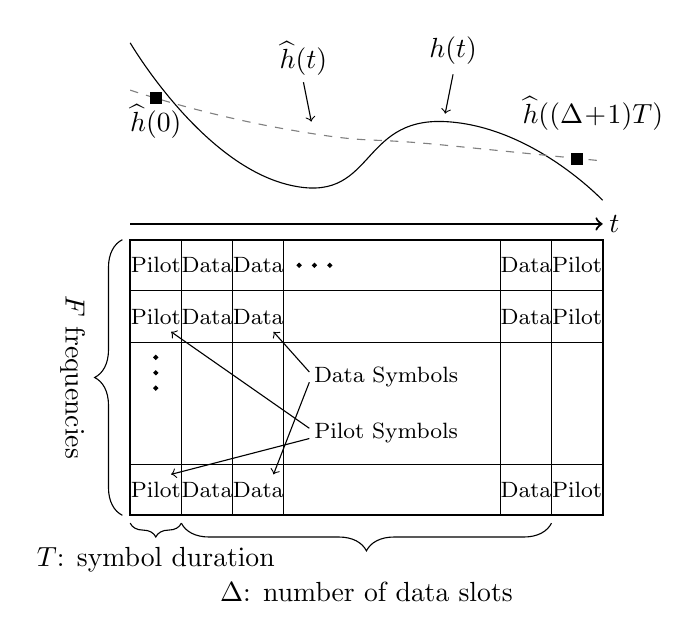
\begin{tikzpicture}[scale = 1]
  \def\x{0.65}
  \def\y{0.07}

  \draw[black, thick] (0,0) rectangle (6,3.5);

  \draw (\x,0) -- (\x,3.5);
  \draw (2*\x,0) -- (2*\x,3.5);
  \draw (3*\x,0) -- (3*\x,3.5);
  \draw (6-\x,0) -- (6-\x,3.5);
  \draw (6-2*\x,0) -- (6-2*\x,3.5);

  \draw (0, \x) -- (6, \x);
  \draw (0, 3.5-\x) -- (6, 3.5-\x);
  \draw (0, 3.5-2*\x) -- (6, 3.5-2*\x);

  \node at (\x/2, \x/2) {\footnotesize Pilot};
  \node at (\x/2, 3.5-\x/2) {\footnotesize Pilot};
  \node at (\x/2, 3.5-3*\x/2) {\footnotesize Pilot};

  \node at (3*\x/2, \x/2) {\footnotesize Data};
  \node at (3*\x/2, 3.5-\x/2) {\footnotesize Data};
  \node at (3*\x/2, 3.5-3*\x/2) {\footnotesize Data};

  \node at (5*\x/2, \x/2) {\footnotesize Data};
  \node at (5*\x/2, 3.5-\x/2) {\footnotesize Data};
  \node at (5*\x/2, 3.5-3*\x/2) {\footnotesize Data};

  \node at (6-3*\x/2, \x/2) {\footnotesize Data};
  \node at (6-3*\x/2, 3.5-\x/2) {\footnotesize Data};
  \node at (6-3*\x/2, 3.5-3*\x/2) {\footnotesize Data};

  \node at (6-\x/2, \x/2) {\footnotesize Pilot};
  \node at (6-\x/2, 3.5-\x/2) {\footnotesize Pilot};
  \node at (6-\x/2, 3.5-3*\x/2) {\footnotesize Pilot};

  \draw [->] (3.5*\x, 1.5*\x) -- (0.8*\x, 0.8*\x);
  \draw [->] (3.5*\x, 1.7*\x) -- (0.8*\x, 3.5-1.8*\x);
  \node at (5*\x, 1.6*\x) {\footnotesize Pilot Symbols};

  \draw [->] (3.5*\x, 2.6*\x) -- (2.8*\x, 0.8*\x);
  \draw [->] (3.5*\x, 2.8*\x) -- (2.8*\x, 3.5-1.8*\x);
  \node at (5*\x, 2.7*\x) {\footnotesize Data Symbols};

  \filldraw [black] (\x/2,3.5-2.3*\x) circle (0.7pt);
  \filldraw [black] (\x/2,3.5-2.6*\x) circle (0.7pt);
  \filldraw [black] (\x/2,3.5-2.9*\x) circle (0.7pt);

  \filldraw [black] (3.3*\x,3.5-\x/2) circle (0.7pt);
  \filldraw [black] (3.6*\x,3.5-\x/2) circle (0.7pt);
  \filldraw [black] (3.9*\x,3.5-\x/2) circle (0.7pt);

  \draw [decorate,decoration={brace,amplitude = 10pt}] (6-\x,-0.1) -- (\x,-0.1)
  node [black,midway,yshift=-25pt] {$\Delta$: number of data slots};
  \draw [decorate,decoration={brace,amplitude = 5pt}] (\x,-0.1) -- (0,-0.1)
  node [black,midway,yshift=-13pt] {$T$: symbol duration};


  \draw [decorate,decoration={brace,amplitude = 10pt}] (-0.1, 0) -- (-0.1,3.5)
  node [black,midway,xshift=-18pt] {\rotatebox{270}{$F$ frequencies}};

  \draw [->, thick] (0,3.7) -- (6,3.7);
  \node at (6.15, 3.7) {$t$};

  \draw plot [smooth, tension=1] coordinates { (0, 6) (2,4.2) (4,5) (6,4)};
  \draw [dashed, gray] plot [smooth, tension=1] coordinates { (0,5.4) (2,4.9) (4,4.7) (6,4.5)};

  \filldraw (\x/2-\y,5.3-\y) rectangle (\x/2+\y, 5.3+\y);
  \node at (\x/2, 5) {$\hat{\mx{h}}(0)$};
  \filldraw (6-\x/2-\y,4.52-\y) rectangle (6-\x/2+\y, 4.52+\y);
  \node at (6.2-\x/2, 5.1) {$\hat{\mx{h}}((\Delta\!+\!1)T)$};

  \draw [->] (4.1,5.6) -- (4,5.1);
  \node at (4.1, 5.9) {$\mx{h}(t)$};

  \draw [->] (2.2,5.5) -- (2.3,5);
  \node at (2.2, 5.8) {$\hat{\mx{h}}(t)$};
\end{tikzpicture}
\caption{Pilot (P) and data (D) symbols in the time-frequency domains of the system in the $(0,(\Delta+1)T)$ interval. The solid line above the
time-frequency resource grid represents the continuous time complex channel $\mx{h}(t)$, while the dashed line represents
the \ac{MMSE} channel estimate $\hat{\mx{h}}(t)$.
Notice that in each time slot of length $T$ all symbols are either pilot or
data symbols.}
\label{fig:Model}
\end{figure}

\begin{table}[t]
\caption{System Parameters}
\vspace{2mm}
\label{tab:notation}
\footnotesize
\begin{tabularx}{\columnwidth}{|X|X|}
\hline
\hline
\textbf{Notation} & \textbf{Meaning} \\
\hline
\hline
% Network layout
$K$ & Number of \ac{MU-MIMO} users \\
\hline
$N_r$ & Number of antennas at the BS \\
\hline
$F$ & Number of frequency channels used for pilot and data transmission within one slot \\
\hline
$\Delta$ & number of data slots in a data-pilot cycle \\
\hline
$\tau_p=F, \tau_d=\Delta F$ & Number of pilot/data symbols within a coherent set of subcarriers  \\
\hline
$\mx{s}\in \mathds{C}^{\tau_p \times 1}$ & Sequence of pilot symbols\\
\hline
$x$ & Data symbol \\
\hline
%$P_p, P, P_{\text{tot}}$ & Pilot power per symbol, data power per symbol, and total power budget  \\
$P_p, P$ & Pilot power per symbol, data power per symbol\\
\hline
$\mx{Y}^p(t) \in \mathds{C}^{N_r \times \tau_p}, y(t) \in \mathds{C}^{N_r}$ & Received pilot and data signal at time $t$, respectively  \\
\hline
% $\mx{N}, \mx{n}_d(t)$ & Additive white Gaussian noise at the received pilot and data signal, respectively \\
% \hline
$\alpha$ & Large scale fading between the mobile station and the base station \\
\hline
$\mx{C} \in \mathds{C}^{N_r \times N_r}$ & Stationary covariance matrix of the fast fading channel \\
\hline
$\mx{h}(t), \hat{\mx{h}}(t) \in \mathds{C}^{N_r}$ & Fast fading channel and estimated channel \\
% $\sigma_p^2 \mx{I}_{N_r}, \sigma_d^2 \mx{I}_{N_r}, \mx{C} \in \mathds{C}^{N_r \times N_r}$
% & Covariance of $\mx{N}$, $\mx{n}_d$, $\mx{h}(t)$, respectively \\
% \hline
\hline
$\bs{\varepsilon}(t) \in \mathds{C}^{N_r}, \bs{\Sigma} \in \mathds{C}^{N_r \times N_r}$
& Channel estimation error and its covariance matrix\\
\hline
%$\mx{G}, \mx{G}^\text{naive}, \mx{G}^\star$ & MU-MIMO receivers: generic, naive, and optimal, respectively. \\
$\mx{G}^\star$ & Optimal MU-MIMO receiver. \\
\hline
$f_D$ & Maximum Doppler frequency \\
\hline
$T$ & Slot duration \\
%\hline
%$\bs{\Lambda}_p$ & AWGN on the received pilot symbols at the \ac{BS} \\
\hline
\end{tabularx}
\end{table}

\subsection{Uplink Pilot Signal Model}
By extending the single antenna channel model of \cite{Savazzi:09},
each transmitting \ac{MS} uses a single time slot to send $F$ pilot symbols,
followed by $\Delta$ time slots, each of which containing $F$ data symbols according to Figure \ref{fig:Model}.
Each symbol is transmitted within a coherent time slot of duration $T$.
Thus, the total frame duration is $(1+\Delta) T$, such that each frame consists of 1 pilot
and $\Delta$ data time slots, which we will index with $i=1 \ldots \Delta$.
User-$k$ transmits each of the $F$ pilot symbols with transmit power $P_{p,k}$, and each data
symbol in slot-$i$ with transmit power $P_k(i),~k=1 \ldots K$.
To simplify notation, in the sequel we tag User-1, and will
drop index $k=1$ when referring to the tagged user.

Assuming that the coherence bandwidth accommodates at least $F$ pilot symbols,
this system allows to create $F$ orthogonal pilot sequences.
To facilitate spatial multiplexing
and \ac{CSIR} acquisition at the \ac{BS}, the \acp{MS} use orthogonal complex
sequences, such as shifted Zadoff-Chu sequences of length $\tau_p=F$, which we denote as:
\begin{align}
\mathbf{s} &\triangleq \left[s_1,...,s_{\tau_p}\right]^T \in \mathds{C}^{{\tau_p \times 1}},
\end{align}
whose elements satisfy %are scaled appropriately according to
$|s_i|^2 = 1$. %, for $i=1,..,\tau_p$ \cite{Sesia:11}.
% To enable spatial multiplexing, the length of the pilot sequences
% $\tau_p$ is chosen such that a maximum of $K$ users can be served simultaneously, implying that
% $\tau_p \geq K$ holds.
Under this assumption, the system can spatially multiplex $K\leq F$ \acp{MS}.
Focusing on the received pilot signal from the tagged user at the \ac{BS},
the received pilot signal takes the form of \cite{Fodor:21}:
\begin{align}
\mathbf{Y}^p(t)
&=
\alpha \sqrt{P_{p}}\mathbf{h}(t) \mathbf{s}^T +\mathbf{N}(t) ~~ \in \mathds{C}^{N_r \times \tau_p},
\label{eqn:received_training_seq}
\end{align}
where %we assume that
$\mathbf{h}(t) \in \mathds{C}^{N_r \times 1} \sim \mathcal{CN}(\mathbf{0},\mathbf{C})$, that is,
$\mathbf{h}(t)$ is a %circular symmetric
complex normal distributed column vector
with mean vector $\mathbf{0}$ and covariance matrix $\mx{C} \in \mathds{C}^{N_r \times N_r}$. % $\in \mathds{C}^{N_r \times N_r}$. %(of size $N_r$), %at all $t$ time instance,
Furthermore, $\alpha$ denotes
% propagation loss
large scale fading, $P_p$ denotes the pilot power of the tagged user,
and $\mathbf{N}(t)\in \mathds{C}^{N_r \times \tau_p}$
is the %spatially and temporally
\ac{AWGN} with element-wise variance $\sigma_p^2$.
It will be convenient to introduce $\mathbf{\tilde Y}^p(t)$ by stacking the columns of  $\mathbf{Y}^p(t)$ as:
\begin{align}
\mathbf{\tilde Y}^p(t)=\textbf{vec}\big(\mathbf{Y}^p(t)\big)=\alpha\sqrt{P_p} \mathbf{S} \mathbf{h}(t) +\mathbf{\tilde N}(t) ~\in \mathds{C}^{\tau_p N_r \times 1},
\label{eqn:received_training_seq2}
\end{align}
where $\textbf{vec}$ is the column stacking vector operator,
$\mathbf{\tilde Y}^p(t)$, $\mathbf{\tilde N}(t) \in \mathds{C}^{\tau_p N_r \times 1}$
and
$\mathbf{S} \triangleq \mathbf{s}\otimes \mathbf{I}_{N_r} \in \mathds{C}^{\tau_p N_r \times N_r}$
is such that $\mathbf{S}^H\mathbf{S}=\tau_p\mathbf{I}_{N_r}$,
where $\mathbf{I}_{N_r}$ is the identity matrix of size $N_r$.
\vspace{-2mm}
\subsection{Channel Model}
\vspace{-1mm}
% Consider a single block of $\Delta$ data symbols sent at time instances $iT$ for $i = 1\ldots \Delta$
% and a pilot symbol sent at time $0$ and subsequently at $(\Delta+1)T$.
In \eqref{eqn:received_training_seq},
the channel $\mx{h}(t)$ evolves continuously according to a multivariate complex stochastic process
with stationary covariance matrix $\mx{C}$.
That is, for symbol duration $T$, the channel ($\mx{h}(t)$) evolves according to the following \ac{AR} process:
\begin{align}
\label{eq:AR1}
\mx{h}(t+T) &= \mx{A} \mx{h}(t) + \bs{\vartheta}(t),
\end{align}
where the transition matrix of the \ac{AR} process is denoted by $\mx{A}$.
This \ac{AR} model has been commonly used to approximate Rayleigh fading channels in e.g. \cite{Baddour05}.
Equation \eqref{eq:AR1} implies that the autocorrelation function of the channel process is:
\begin{align}
\mathds{E}\left(\mx{h}(t)\mx{h}^H(t+iT)\right) &= \mx{C}\left(\mx{A}^H\right)^i, \quad \forall i.
\end{align}
%satisfies the following equation:
Consequently, the autocorrelation function of
the fast fading channel ($\mx{h}(t)$) is modelled as:
\begin{align}
\label{eq:autocorr}
\mx{R}(i) \triangleq
\mathds{E}\left(\mx{h}(t)\mx{h}^H(t+iT)\right) &= \mx{C} e^{\mx{Q}^H i T },
\end{align}
where matrix $\mx{Q}$ describes the correlation decay, such that:
\begin{align}
e^{\mx{Q}T} = \mx{A}.
\end{align}

Similarly, for user $k$,
\begin{align}
\label{eq:autocorrk}
\mx{R}_k(i) \triangleq
\mathds{E}\left(\mx{h}_k(t)\mx{h}_k^H(t+iT)\right) &= \mx{C}_k e^{\mx{Q}_k^H i T },
\end{align}

%We denote by $R(i) \triangleq cJ_0(2 \pi f_D i T)$ the correlation between the $i$-th element of
%the channel vectors that are $i \cdot T$ apart from each other in time.
% For the pilot channels we
In each pilot slot,
the \ac{BS} utilizes \ac{MMSE} channel estimation to obtain the channel estimate of each user, as it will be detailed in Section \ref{Sec:ChannelE}.
Without loss of generality, to simplify the notation, hereafter we assume that the time unit is $T$ and $iT=i$.

\begin{comment}
\begin{align}
\label{eq:LS}
\hat{\mx{h}}(t) &= \mx{h}(t) + \boldsymbol{\varepsilon}(t), \\
\boldsymbol{\varepsilon}(t) & \sim
%\mathcal{CN}\left(0,\frac{\boldsymbol{\Lambda}_p}{\alpha^2 F P_p} \right) \triangleq
\mathcal{CN}\left(0,\mx{\Sigma}\right)
\text{~with~} \mx{\Sigma} = \frac{\boldsymbol{\Lambda}_p}{\alpha^2 F P_p}
\end{align}
where $\mathcal{CN}\left(0,\mx{\Sigma}\right)$ is the $N_r$ dimensional complex normal distribution with mean $0$ and covariance matrix $\mx{\Sigma}$,  $\boldsymbol{\Lambda}_p$ is the covariance matrix of the \ac{AWGN} on the pilot symbols at the receiver
and $\alpha$ is the path loss between the \ac{MS} and the \ac{BS} \cite{Fodor:21}, which are assumed to be identical for all $F$ frequencies.
\end{comment}


\subsection{Data Signal Model}
When spatially multiplexing $K$ \ac{MU-MIMO} users,
the received data signal at the \ac{BS} at time $t$ is \cite{Fodor:21}:

\begin{align}
\mathbf{y}(t)
&=
\underbrace{\mathbf{\alpha} \mathbf{h}(t) \sqrt{P} x(t)}_{\text{tagged user}}
+ \underbrace{\sum_{k=2}^K \mathbf{\alpha}_{k} \mathbf{h}_k(t) \sqrt{P_{k}} x_{k}(t)}_{\text{co-scheduled MU-MIMO users}}
% \underbrace{\sum_{i \neq 1}^L \sum_{k=1}^K \mathbf{g}_{1,i,k} \sqrt{P_{i,k}} x_{i,k}}_{\text{Other cells}}
+\mathbf{n}_d(t),
%~~\in \mathds{C}^{N_r \times 1},
\label{eq:mumimo2}
\end{align}
\noindent where $\mathbf{y}(t)\in \mathds{C}^{N_r \times 1}$;
% and $\mathbf{\alpha}_{k} \mathbf{h}_k(t) \in \mathds{C}^{N_r \times 1}$
% denotes the channel vector,
and $x_k(t)$ denotes the transmitted data symbol of User-$k$
at time $t$ with transmit power $P_k$.
Furthermore, $\mathbf{n}_d(t)~\sim \mathcal{CN}\left(\mx{0},\sigma_d^2 \mathbf{I}_{N_r}\right)$
is the \ac{AWGN} at the receiver.
\vspace{-2mm}
\section{Channel Estimation}
\label{Sec:ChannelE}
In this section, we are interested in calculating the \ac{MMSE} estimation of the
channel in each slot $i$, based on received pilot signals, as a function of the frame
size corresponding to pilot spacing (see $\Delta$ in Figure \ref{fig:Model}).
Note that estimating the channel at the receiver can be based on
multiple received pilot signals both before and after the actual data slot $i$.
While using pilot signals that are received before data slot $i$ requires to
store the samples of the received pilot, using pilot signals that arrive after
data slot $i$ necessarily induces some delay in estimating the transmitted data symbol.
In the numerical section, we will refer to specific channel estimation strategies
as, for example, "1 before, 1 after" or "2 before, 1 after" depending on the number
of utilized pilot signals received prior to or following data slot $i$
for \ac{CSIR} acquisition.
In the sequel we use the specific case of "2 before, 1 after" to illustrate the
operation of the \ac{MMSE} channel estimation scheme,
that is when the receiver uses the pilot signals
$\mathbf{\tilde Y}^p(-\Delta-1)$, $\mathbf{\tilde Y}^p(0)$, and $\mathbf{\tilde Y}^p(\Delta+1)$
for \ac{CSIR} acquisition.
We are also interested in determining the distribution of the
resulting channel estimation error, whose covariance matrix, denoted by
$\mx{Z}(\Delta,i)$, will play an important role in subsequently determining
the deterministic equivalent of the \ac{SINR}.
\vspace{-2mm}
\subsection{\ac{MMSE} Channel Estimation and Channel Estimation Error}
As illustrated in Figure \ref{fig:Model},
in each data slot $i$, the \ac{BS} utilizes the \ac{MMSE} estimates of the channel
obtained in the neighboring pilot slots, for example at $(-\Delta-1)$, $0$ and $(\Delta+1)$, %according to \eqref{eqn:received_training_seq2}.
using the respective received pilot signals according to \eqref{eqn:received_training_seq2}, that is
$\mathbf{\tilde Y}^p\big((-\Delta-1)\big)$, $\mathbf{\tilde Y}^p(0)$ and $\mathbf{\tilde Y}^p\big((\Delta+1)\big)$, using the following lemma.

\begin{lem}
\label{lem:mmsechannel}	
The \textup{MMSE} channel estimator approximates the autoregressive fast fading channel in time slot $i$
based on the received pilots at $(-\Delta-1)$, $0$ and $(\Delta+1)$ as
\begin{align}
\label{eq:hmmse}
&\mathbf{\hat h}_{\textup{MMSE}}(\Delta,i)=
\mx{H^\star}(\Delta,i) \mathbf{\hat Y}^p(\Delta),
\end{align}
where
\begin{align*}
\mx{H^\star}(\Delta, i) = \frac{1}{\alpha \sqrt{P_p} \tau_p} \mx{E}(\Delta,i). \big(\mx{M}(\Delta)+\mx{\Sigma}_3\big)^{-1}.(\mx{s}^H\otimes \mx{I}_{3N_r}),
\end{align*}

$\mathbf{\hat Y}^p(\Delta) \triangleq \begin{bmatrix}
\mathbf{\tilde Y}^p((-\Delta-1)) \\
\mathbf{\tilde Y}^p(0) \\
\mathbf{\tilde Y}^p((\Delta+1))
\end{bmatrix}$~~and~~$\mx{\Sigma}_3\triangleq \frac{\sigma_p^2}{\alpha^2P_p \tau_p} \mx{I}_{3N_r}$,
\begin{align}
\label{eq:E}
\mx{E}(\Delta,i) &\triangleq
\begin{bmatrix}
\mx{R}(\Delta \!+\! 1 \!+\! i) & \mx{R}(i) &
\mx{R}(\Delta \!+\! 1 \!-\! i)
\end{bmatrix},
\\
\label{eq:M}
\mx{M}(\Delta) &\triangleq
\begin{bmatrix}
\mx{C} & \mx{R}(\Delta \!+\! 1) & \mx{R}(2\Delta \!+\! 2)  \\
\mx{R}^H(\Delta \!+\! 1) & \mx{C} & \mx{R}(\Delta \!+\! 1) \\
\mx{R}^H(2\Delta \!+\! 2) & \mx{R}^H(\Delta \!+\! 1) & \mx{C}\\
\end{bmatrix}.
\end{align}

\end{lem}

\begin{proof}
The \ac{MMSE} channel estimator aims at minimizing the \ac{MSE} between the channel estimate
$\mathbf{\hat h}_{\textrm{MMSE}}(\Delta, i) = \mathbf{H}^\star(\Delta, i) \mathbf{\hat Y}^p(\Delta)$ and the channel $\mathbf{h}(i)$, that is
\begin{align}
\mathbf{H^\star}(\Delta, i)= \text{arg} \min_{\mathbf{H}} \mathds{E}_{\mathbf{h},\mathbf{n}}\{ ||\mathbf{H} \mathbf{\hat Y}^p(\Delta) - \mathbf{h}(i)||^2 \}.
\end{align}
The solution of this quadratic optimization problem is
$\mathbf{H^\star}(\Delta, i)= \mx{a}(\Delta, i)^H \mx{F}^{-1}(\Delta)$
with
\begin{align}
\label{eq:Fandb}
\mx{F}(\Delta) &\triangleq \mathds{E}_{\mathbf{h},\mathbf{n}}\left(\mx{\hat Y}^p(\Delta) \left(\mx{\hat Y}^p(\Delta)\right)^H\right), \\
\mx{a}(\Delta, i) &\triangleq \mathds{E}_{\mathbf{h},\mathbf{n}}\left( \mx{\hat Y}^p(\Delta) \mx{h}^{H}(i)\right).
\end{align}
Let
\begin{align}
\mx{\bar h}(\Delta) \triangleq \begin{bmatrix}
\mx{h}((-\Delta-1)) \\
\mx{h}(0) \\
\mx{h}((\Delta+1))
\end{bmatrix} \nonumber
\end{align}
and
\begin{align}
\mx{\tilde{\bar{N}}}(\Delta) \triangleq \begin{bmatrix}
\mx{\tilde{N}}((-\Delta-1)) \\
\mx{\tilde{N}}(0) \\
\mx{\tilde{N}}((\Delta+1))
\end{bmatrix}.
\end{align}
Using $\mx{\bar h}(\Delta)$, we have
\begin{align}
\begin{bmatrix}
\mx{S}\mx{h}((-\Delta-1)) \\
\mx{S}\mx{h}(0) \\
\mx{S}\mx{h}((\Delta+1))
\end{bmatrix}=
\begin{bmatrix}
\mx{S}  & \mx{0} & \mx{0} \\
\mx{0} & \mx{S}  & \mx{0} \\
\mx{0} & \mx{0} & \mx{S}
\end{bmatrix}\mx{\bar h}(\Delta)
\nonumber \\
~~~~~~~~= (\mx{I}_3\otimes\mx{S}) \mx{\bar h}(\Delta)=  (\mx{s}\otimes \mx{I}_{3N_r}) \mx{\bar h}(\Delta).
\end{align}
Since $\mx{\bar h}(\Delta)$ and $\mx{\tilde{\bar{N}}}(\Delta)$ are independent and
\begin{align}
\mathds{E}_{\mathbf{h},\mathbf{n}}(\mx{\bar h}(\Delta)\mx{\bar h}^H(\Delta))&=\mx{M}(\Delta),\\
\mathds{E}_{\mathbf{h},\mathbf{n}}(\mx{h}(i)\mx{\bar h}^H(\Delta))&=\mx{E}(\Delta,i).
\end{align}
Therefore, for $\mx{F}(\Delta)$ and $\mx{a}(\Delta,i)$, we have
\begin{align*}
\mx{F}(\Delta) &=
%\mathds{E}_{\mathbf{h},\mathbf{n}}\left(\mx{\tilde{\bar{Y}}}^p\mbox{$\mx{\tilde{\bar{Y}}}^p$}^H\right)\\&=
\mathds{E}_{\mathbf{h},\mathbf{n}}
\left(\left(\alpha\sqrt{P_p} (\mx{I}_3\otimes\mx{S}) \mx{\bar{h}}(\Delta) +\mx{\tilde{\bar{N}}}(\Delta)\right)\right.\nonumber \\
&~~~~~~~~~~~~\cdot \left.\left(\alpha\sqrt{P_p} (\mx{I}_3\otimes\mx{S}) \mx{\bar{h}}(\Delta) +\mx{\tilde{\bar{N}}}(\Delta)\right)^H\right)\\
&=\alpha^2P_p(\mx{I}_3\otimes\mx{S})\mx{M}(\Delta)\left(\mx{I}_3\otimes\mx{S}^H\right)+ \sigma_p^2 \mathbf{I}_{3N_r\tau_p},\\
\mx{a}(\Delta, i) &= \mathds{E}_{\mathbf{h},\mathbf{n}}\left( \mx{\hat Y}(\Delta) \mx{h}^{H}(i)\right) \\
&=\mathds{E}_{\mathbf{h},\mathbf{n}}
\left(\left(\alpha\sqrt{P_p} (\mx{I}_3\otimes\mx{S}) \mx{\bar{h}}(\Delta) +\mx{\tilde{\bar{N}}}(\Delta)\right)
\mx{h}^{H}(i)\right)\\
&= \alpha\sqrt{P_p} ~(\mx{I}_3\otimes\mx{S})~\mx{E}(\Delta,i)^T,
\end{align*}
which yields Lemma \ref{lem:mmsechannel}.
\end{proof}

The \ac{MMSE} estimate of the channel is then expressed as:
\begin{align}
\nonumber
&\mathbf{\hat h}_{\textrm{MMSE}}(\Delta, i)=\mathbf{H^\star}(\Delta, i) \mathbf{\hat Y}^p(\Delta) ~~~~ \\
&~~~~=\mathbf{H^\star}(\Delta, i)
\left(\alpha\sqrt{P_p} (\mx{I}_3\otimes\mx{S}) \mx{\bar{h}}(\Delta) +\mx{\tilde{\bar{N}}}(\Delta)\right)
\nonumber
\\
&~~~~=
\frac{1}{\alpha\sqrt{P_p} \tau_p}
\mx{E}(\Delta, i) \left(   \mx{M}(\Delta) + \mx{\Sigma}_{3} \right)^{-1}
\nonumber
\\&~~~~~~~~~~.
\left(\alpha\sqrt{P_p} \tau_p \mx{\bar{h}}(\Delta) + \left(\mx{I}_3 \otimes \mx{S}^H\right) \mx{\tilde{\bar{N}}}(\Delta)\right).
\label{eq:MMSEt}
\end{align}

Next, we are interested in deriving the distribution of the estimated channel and
the channel estimation error, since these will be important for understanding the
impact of pilot spacing on the achievable \ac{SINR} and spectral efficiency of
the \ac{MU-MIMO} system. To this end, the following two corollaries of
Lemma \ref{lem:mmsechannel} and \eqref{eq:MMSEt} will be important in the sequel.
\begin{cor}
\label{cor:rmmse}	
The estimated channel $\mathbf{\hat h}_{\textup{MMSE}}(\Delta, i)$ is a circular symmetric complex normal distributed vector
$\mathbf{\hat h}_{\textup{MMSE}}(\Delta, i) \sim %\mathcal{CN}(\mathbf{0},\mathbf{R}_{\textup{MMSE}}(\Delta, i))$,
\mathcal{CN}\Big(\mathbf{0},\mathbf{\hat \Phi}_{\textup{MMSE}}(\Delta, i)\Big)$,
with
\begin{align}
\label{eq:rmmse}
\mathbf{\hat \Phi}_{\textup{MMSE}}(\Delta, i) \triangleq
& \mathds{E}_{\mathbf{h},\mathbf{n}} \{\mathbf{\hat h}_{\textup{MMSE}}(\Delta, i) \mathbf{\hat h}_{\textup{MMSE}}^H(\Delta, i)\}
 \nonumber \\
=& \mx{E}(\Delta, i) \big(\mx{M}(\Delta)+\mx{\Sigma}_3\big)^{-1} \mx{E}(\Delta, i)^H.
\end{align}

\end{cor}

\begin{proof}
Equation \eqref{eq:rmmse} follows directly from \eqref{eq:MMSEt}.	
\end{proof}

An immediate consequence of Corollary \ref{cor:rmmse}
is the following corollary regarding the covariance of the channel estimation
error, as a function of pilot spacing.
\begin{cor}
\label{Cor:ChEstError}
The channel estimation error in slot $i$, $\mx{\hat{h}}_{\textup{MMSE}}(\Delta, i)-\mx{h}(\Delta, i)$,
is complex normal distributed with zero mean vector and
covariance matrix given by:
\begin{align}
\label{eq:Z}
\mx{Z}(\Delta, i) \triangleq  \mx{C} -
\mx{E}(\Delta, i) \big(\mx{M}(\Delta)+\mx{\Sigma}_3\big)^{-1}
\mx{E}(\Delta, i)^H.
\end{align}
\end{cor}

In the following section we will calculate the \ac{SINR} of the received data symbols.
For simplicity of notation, we use $\mx{\hat h}_{\textup{MMSE}}(\Delta, i)=\mx{\hat h}(\Delta, i)$, and  introduce
$$\mx{b}(\Delta, i) \triangleq \alpha\sqrt{P(i)}\mx{\hat{h}}(\Delta, i)$$
with covariance matrix
\begin{align}
\label{eq:Phi}
\bs{\Phi}(\Delta, i) & \triangleq
\mathds{E}\left( \mx{b}(\Delta, i)\mx{b}^H(\Delta, i) \right)  \nonumber \\
&=\mathds{E}\left( \Big(\alpha\sqrt{P(i)} \mx{\hat{h}}(\Delta, i) \Big)\Big(\alpha\sqrt{P(i)} \mx{\hat{h}}(\Delta, i) \Big)^H  \right)  \nonumber \\
&=\alpha^2P(i)(\mx{C}-\mx{Z}(\Delta, i)).
\end{align}
% \dg{For consistency, shouldn't we use $P_i$ instead of $P(i)$?}
\subsection{Summary}

This section derived the \ac{MMSE} channel estimator (Lemma \ref{lem:mmsechannel})
that uses the received pilot signals
both before and after a given data slot $i$ and depends on the frame size $\Delta$ (pilot spacing).
As important corollaries of the channel estimation scheme, we established the distribution
of both the estimated channel (Corollary \ref{cor:rmmse})
and the associated channel estimation error in each data
slot $i$ (Corollary \ref{Cor:ChEstError}), as functions of both the employed pilot spacing and pilot power. These
results serve as a starting point for deriving the achievable \ac{SINR} and spectral
efficiency.

\section{\ac{SINR} Calculation}
\label{Sec:SINR}

\subsection{Instantaneous \ac{SINR}}
We start with recalling an important lemma from \cite{Fodor:22}, which calculates the instantaneous \ac{SINR}
in an \ac{AR} fast fading environment
when the \ac{BS} uses the \ac{MMSE} estimation of the fading channel, and employs the optimal linear
receiver:
\begin{align}
\label{eq:Gstar2}
\mx{G}^\star(\Delta, i) &=
% \textup{arg} \min_{\mx{G}} \textup{MSE}\left(\mx{G},\mx{\hat H}(t), \mx{\hat H}(t-1)\right)
\mx{b}^H(\Delta,i) \mx{J}^{-1}(\Delta,i),
\end{align}
where $\mx{J}(\Delta, i) \in \mathds{C}^{N_r \times N_r}$
is defined as
\begin{align}
%\label{eq:A3}
\nonumber
\mx{J}(\Delta, i)
&\triangleq
\sum_{k=1}^K  \mx{b}_k(\Delta, i) \mx{b}_k^H(\Delta, i) + \bs{\beta}(\Delta, i),
\end{align}
where
\begin{align}
\label{eq:beta}
\bs{\beta}(\Delta, i) \triangleq \sum_{k=1}^K \alpha_k^2 P_k  \mx{Z}_k(\Delta, i) + \sigma^2_d \mx{I}_{N_r}.
\end{align}
%and $\mx{I}$ is the identity matrix of size $N_r$.

When using the above receiver, which minimizes the \ac{MSE} of the received data symbols in the
presence of channel estimation errors, the following result from \cite{Fodor:22} will be useful in the sequel:
\begin{lem}[See \cite{Fodor:22}, Lemma 3]
Assume that
the receiver employs \textup{\ac{MMSE}} symbol estimation,
that is it employs the optimal linear receiver $\mx{G}^\star(\Delta, i)$ given in \eqref{eq:Gstar2}. %and the instantaneous channel estimates,
Then the instantaneous \textup{\ac{SINR}} of the estimated data symbols of the tagged user,
$\gamma(\Delta, i)$ %\Big(\mathbf{G}^\star, \hat{\mathbf{H}}(t),\hat{\mathbf{H}}(t-1)\Big)$
is given as:
% the instantaneous \textup{\ac{SINR}} of the data symbols, can be expressed as:
%
\begin{equation}
\label{eq:lemma2Eq}
\gamma(\Delta, i) %\Big(\mathbf{G}^\star(t), \hat{\mathbf{H}}(t),\hat{\mathbf{H}}(t-1)\Big)
=
\mx{b}^H(\Delta, i) \mathbf{\bar{J}}^{-1}(\Delta, i) \mx{b}(\Delta, i),
\end{equation}
where
\vspace{-1mm}
\begin{equation}
\mathbf{\bar{J}}(\Delta, i) \triangleq \mathbf{J}(\Delta, i)- \mx{b}(\Delta, i)\mx{b}^H(\Delta, i).
\end{equation}
\end{lem}
\begin{comment}
Using the \ac{MMSE} estimate $\bar{\mx{h}}(i) = \mx{E}(i) \mx{\hat{\bar{h}}}(\Delta)$ of the channel $\mx{h}(i)$,
we can calculate the \ac{SINR} of the estimated data symbol sent at time $i$ when the \ac{BS} employs an optimal linear receiver as provided in \cite{Fodor:22}.
Lemma 2 in \cite{Fodor:22} shows that when $K$ \acp{MS} enumerated $k = 1 \ldots K$ transmit data signals
through channels $\mx{h}_k$ with \ac{MMSE} estimates
$\bar{\mx{h}}_k$, estimation error covariance $\mx{Z}_k$, path losses $\alpha_k$,
and employing transmit powers $P_k$, the \ac{SINR} of the estimated data symbol of user $k$, $\hat x = \mx{G}\mx{y}$:

\begin{align}
    \gamma_k = \alpha_k^2 P_k \bar{\mx{h}}_k^H \left( \sum_{l \neq k}^K \alpha_l^2 P_l \bar{\mx{h}}_l\bar{\mx{h}}_l^H
    + \sum_{l = 1}^K \alpha_l^2 P_l \mx{Z}_l + \sigma_d^2 \mx{I} \right)^{-1}\bar{\mx{h}}_k,
\end{align}

where $\sigma_d^2$ is the variance of the \ac{AWGN} on the data signal.
Applying this formula on the previous section, where the data symbol of User-$k$, in data time slot $i$ is transmitted through the channel $\mx{h}_k(iT)$,
with \ac{MMSE} estimate $\bar{\mx{h}}_k(iT) = \mx{E}_k(i) \bs{\zeta}_k(\Delta)$ and channel covariance matrix $\mx{Z}(i)$
the \ac{SINR} of the estimated data symbol sent by User-$k$ is given by
\end{comment}
For the \ac{AR} fading case considered in this paper,
based on the definitions of $\mx{b}(\Delta, i)$, $\mx{J}(\Delta, i)$ and $\mx{\bar{J}}(\Delta, i)$,
the instantaneous \ac{SINR} of the tagged user is then expressed as:
\begin{align}
\gamma(i) &  =  \mx{b}^H(\Delta, i) \mathbf{\bar{J}}^{-1}(\Delta, i) \mx{b}(\Delta, i)
  \nonumber\\
 &=
\textup{tr}\left( \mx{b}(\Delta, i)\mx{b}^H(\Delta, i) \mathbf{\bar{J}}^{-1}(\Delta, i) \right).
\end{align}

\subsection{Slot-by-Slot Deterministic Equivalent of the \ac{SINR} as a Function of Pilot Spacing $\Delta$}
We can now prove the following important proposition that gives the asymptotic deterministic equivalent
of the instantaneous \ac{SINR} in data slot $i$, $\bar{\gamma}(\Delta, i)$, when the number of antennas $N_r$ approaches infinity.
This asymptotic equivalent \ac{SINR} gives a good approximation of averaging the instantaneous \ac{SINR} of the tagged user \cite{Wagner:2012, Hoydis:13, Fodor:22}.

\begin{prop}
\label{Prop:SINR}
% According to this theorem, for User-$1$ the \ac{SINR} is given by
The asymptotic deterministic equivalent \ac{SINR} of the tagged user in data slot $i$ can be calculated as:
\begin{align}
\label{eq:hoydis1}
\bar{\gamma}(\Delta, i) &= \textup{tr}\Big( \bs{\Phi}(\Delta, i)\mx{T}(\Delta, i)  \Big),
\end{align}
where $\mx{T}(\Delta, i)$ is defined as: %given by
\begin{align}
\label{eq:hoydis2}
\mx{T}(\Delta, i) \triangleq \left( \sum_{m = 2}^{K} \frac{\bs{\Phi}_m(\Delta, i)}{1 + \delta_m(\Delta, i)} + \bs{\beta}(\Delta, i) \right)^{-1},
\end{align}
and $\delta_m(\Delta, i)$ are the solutions of the following system of $K$ equations
\begin{align}
\label{eq:hoydis3}
\delta_m(\Delta, i) &= \textup{tr}\left(\bs{\Phi}_m(\Delta, i)
\left( \sum_{l = 2}^{K} \frac{\bs{\Phi}_l(\Delta, i)}{1 + \delta_l(\Delta, i)} + \bs{\beta}(\Delta, i)  \right)^{-1} \right)
\end{align}
for $\forall m = 1, \ldots, K$.
\end{prop}
The above system of $K$ equations gives the deterministic equivalent of the \ac{SINR} of the tagged user,
and a different set of $K$ equations must be used for each user.
\begin{proof}
The $\mx{b}_k(\Delta, i)$ vectors are independent for $k = 1 \ldots K$,
and the covariance matrix of $\mx{b}_k(\Delta, i)$ is $\bs{\Phi}_k(\Delta, i)$
(c.f. \eqref{eq:Phi}).
We can then express the expected value of the \ac{SINR} of the tagged user as follows:
\begin{align}
\label{eq:gammaB}
& \bar{\gamma}(\Delta, i) \triangleq \mathds{E}\Big(\gamma(\Delta, i)\Big)   \\
&= \mathds{E}\left( \textup{tr}\left( \bs{\Phi}(\Delta, i)  \left( \sum_{l = 2}^K  \mx{b}_l(\Delta, i) \mx{b}_l^H(\Delta, i)  +\bs{\beta}(\Delta, i) \right)^{\!\!-1}  \right) \right).
\nonumber
\end{align}
%We proceed
The proposition is established
by invoking Theorem \ref{thm:upperbound} in \cite{Wagner:2012}, which is applicable in multiuser systems and
% Theorem \ref{thm:upperbound} in \cite{Wagner:2012}
gives the value of the deterministic equivalent of $\bar{\gamma}(\Delta, i)$
implicitly using a system of $K$ equations and noticing that
$\bar{\gamma}(\Delta, i) = \delta_1(\Delta, i)$, since $\delta_1(\Delta, i)=\textup{tr}\big( \bs{\Phi}(\Delta, i) \mx{T}(\Delta, i)\big)$ according to \eqref{eq:hoydis3}.
\end{proof}

\subsection{Summary}
This section established the instantaneous slot-by-slot \ac{SINR} of a tagged user ($\bar \gamma(i)$) of a \ac{MU-MIMO} system operating over %continuous time
a fast fading channels modelled as \ac{AR} processes,
by applying our previous result obtained for discrete-time \ac{AR} channels
reported in \cite{Fodor:21}.
Next, we invoked Theorem \ref{thm:upperbound} in \cite{Wagner:2012}, to establish the deterministic
equivalent \ac{SINR} for each slot, as a function of the frame size (pilot spacing) $\Delta$, see Proposition \ref{Prop:SINR}.
These results serve as a basis for formulating the pilot spacing optimization problem over the frame size and pilot power as optimization variables.

\section{Pilot Spacing and Power Control}
\label{Sec:PilotSpacing}
In this section, we study the impact of pilot spacing and power control on the achievable \ac{SINR}
and the \ac{SE} of all users in the system.
The asymptotic \ac{SE} of the $i$-th data symbol of user $k$ is
\begin{align}
\label{eq:SE}
\text{SE}_k(\Delta, i) \triangleq \log\Big(1 + \bar{\gamma}_k(\Delta, i)\Big),
\end{align}
where $\bar{\gamma}_k(\Delta, i)$ denotes the average \ac{SINR} of  user $k$ when sending the $i$-th data symbol, and when $\Delta$ data symbols are sent between every pair of pilot symbols.
Consequently, the %information rate
average \ac{SE}
of  user $k$ over the $(\Delta+1)$ slot long frame is
\begin{align}
\frac{\sum_{i=1}^{\Delta}\text{SE}_k(\Delta, i)}{\Delta + 1},
\end{align}
which can be optimized over $\Delta$.
More importantly, %the sum information rate
the aggregate average \ac{SE}
of the \ac{MU-MIMO} system for the $K$ users can be expressed as:
\begin{align}
\text{SE}(\Delta) = \frac{\sum_{k=1}^K \sum_{i=1}^{\Delta}\text{SE}_k(\Delta,i)}{\Delta + 1}.
\label{eq:multiopt}
\end{align}


\subsection{An Upper Bound of the Deterministic Equivalent \ac{SINR} and the \ac{SE}}

Let us assume that $\mx{Q}_k=q_k \mx{I}_{N_r}$, that is the
channel vector $\mx{h}_k(t)$ consists of independent \ac{AR} processes in the spatial domain, implying that:
\begin{align}
\label{eq:r1}
\mx{R}_k(i) \triangleq
\mathds{E}\left(\mx{h}_k(t)\mx{h}_k^H(t+i)\right) &= \mx{C}_k e^{q_k^* i},
\end{align}
where $q_k$ is a scalar, $q_k^*$ denotes complex conjugation, and let $\bar{q}_k\triangleq Re(q_k)<0$.

Note that the exponential approximation of the autocorrelation function of the fast fading process expressed
in \eqref{eq:r1} is related to the Doppler frequency of Rayleigh fading through:
\begin{align}
\label{eq:RayleighApprox}
\underbrace{\mx{C}J_0(2 \pi f_D i)}_{\text{True autocorrelation of Rayleigh fading}} &\approx \mx{R}(i),
\end{align}
where $J_0(.)$ is the zeroth order Bessel function \cite{Wang:03}.
Based on the exponential approximation of this Rayleigh fading process in \eqref{eq:r1}, the Doppler frequency of the approximate model is obtained from $2 \pi f_D i = Re(q_k^* i)$, i.e. $f_D = 2 \pi/\bar{q}_k$.

To optimize \eqref{eq:multiopt}, we first find an upper bound of $\text{SE}_k(\Delta,i)$
via an upper bound of $\bar{\gamma}_k(\Delta, i)$.
To simplify the notation, the following discussion refers to the tagged user, and later we utilize that the same relations hold for all users.
We introduce the following upper bound of $\bar{\gamma}(\Delta, i)$:
\begin{align}
\label{eq:upper}
\bar{\gamma}^{(u)}(\Delta, i) \!&\triangleq \textup{tr}\!\left(\! \bs{\Phi}^{(u)}(\Delta, i)  \left(\sum_{l = 1}^K \!\alpha_l^2 P_l \mx{Z}^{(u)}_l(\Delta, i) \!+\! \sigma_d^2 \mx{I_{N_r}}\right)^{\!\!\!-1}  \!\right)\!,
\end{align}
where $\mx{Z}^{(u)}(\Delta, i)$ and $\bs{\Phi}^{(u)}(\Delta, i)$ are given by
\begin{align}
\label{eq:zu}
\mx{Z}^{(u)}(\Delta, i) &\triangleq \mx{C} - \rho(\Delta, i) \mx{C} \left(\eta  \mx{C} + \bs{\Sigma} \right)^{-1} \mx{C},  \\
\label{eq:phiu}
\bs{\Phi}^{(u)}(\Delta, i) &\triangleq \alpha^2 P \rho(\Delta, i) \mx{C} \left( \eta \mx{C} + \bs{\Sigma} \right)^{-1} \mx{C},
\end{align}
with $\eta$ being a constant, $\mx{\Sigma}\triangleq \frac{\sigma_p^2}{\alpha^2P_p \tau_p} \mx{I}_{N_r}$ and
\begin{align}
\label{eq:rho}
%\mx{\Sigma} &\triangleq \frac{\sigma_p^2}{\alpha^2P_p %\tau_p} \mx{I}_{N_r} \\
\rho(\Delta, i) &\triangleq e^{2\bar{q} (\Delta + 1 + i)} + e^{2\bar{q}  i} + e^{2\bar{q} (\Delta + 1 - i)}.
\end{align}

\begin{thm}
\label{thm:upperbound}
If $\bar{q}<0$ and
\begin{align}
\label{eq:etacond}
0<\eta<\frac{1}{2}\left(2+a^2-a\sqrt{8+a^2}\right),
\end{align}
with $a\triangleq e^{2\bar{q}}$
then  $\bar{\gamma}(\Delta, i)\leq \bar{\gamma}^{(u)}(\Delta, i)$.
\end{thm}
%\overset{(a)}{=}
\begin{proof}
We prove the theorem based on the following inequalities
\begin{align}
\bar{\gamma}(\Delta, i)
&\overset{(a)}{\leq}
\textup{tr}\left( \bs{\Phi}(\Delta, i) \bs{\beta}(\Delta, i)^{-1} \right) \nonumber \\
&\overset{(b)}{\leq}
   \textup{tr}\left( \bs{\Phi}^{(u)}(\Delta, i) \bs{\beta}(\Delta, i)^{-1} \right)
\overset{(c)}{\leq}
   \bar{\gamma}^{(u)}(\Delta, i),  \label{eq:gammabound}
\end{align}
which are proved in consecutive lemmas.
\end{proof}

%The following properties of positive semi-definite matrices are essential to prove the theorem.
\begin{lem}
\label{lem:AB}
Let $\mx{A}$, $\mx{B}$ and $\mx{C}$ be positive definite matrices and $\mx{D}$ be any matrix, such that $\mx{A} \preceq \mx{B}$ (i.e. $\mx{B}-\mx{A}$ is a positive semidefinite matrix), then
\begin{align}
\label{eq:ABinv}
\mx{A}^{-1} &\succeq \mx{B}^{-1},
\\
\label{eq:AB3}
\textup{tr}\left( \mx{D}^H \mx{A} \mx{D} \right) &\leq \textup{tr}\left(\mx{D}^H \mx{B} \mx{D} \right) \\
\label{eq:AB1}
\textup{tr}\left( \mx{A} \mx{C} \right) &\leq \textup{tr}\left(\mx{B} \mx{C} \right)
\\
\label{eq:AB2}
\textup{tr}\left( \mx{C} \mx{A}^{-1} \right) &\geq \textup{tr}\left( \mx{C} \mx{B}^{-1} \right).
\end{align}
\end{lem}
\begin{proof}
$\mx{A}^{-1} \succeq \mx{B}^{-1}$ is given in \cite[p. 495, Corollary 7.7.4(a)]{Horn2013}.
\eqref{eq:AB3} follows from the fact that $\mx{D}^H (\mx{B}-\mx{A}) \mx{D}$ is a positive semidefinite matrix since $\mx{B}-\mx{A}$ is a positive semidefinite matrix and
for any $\mx{x}$
\begin{align}
\mx{x}^H \mx{D}^H (\mx{B}-\mx{A}) \mx{D} \mx{x} = \mx{y}^H (\mx{B}-\mx{A}) \mx{y} \geq 0
\end{align}
where $\mx{y} \triangleq \mx{D} \mx{x}$.
Let $\mx{C}=\mx{D}^H \mx{D}$ be the Cholesky decomposition of $\mx{C}$ then
\eqref{eq:AB1} and \eqref{eq:AB2} follows from \eqref{eq:AB3}, by utilizing the cyclic property of the trace operator.
\end{proof}

\begin{lem}
\label{lem:beta}
For $\bar{q}<0$ and $\eta$ satisfying \eqref{eq:etacond},
the following relation holds
\begin{align}
&\mx{E}(\Delta, i) \big(\mx{M}(\Delta,i)+\mx{\Sigma}_3\big)^{-1} \mx{E}(\Delta, i)^H
\nonumber \\&
~~~~~~~~~~~~~~\preceq \rho(\Delta, i) \mx{C} \left( \eta \mx{C} \!+\! \bs{\Sigma} \right)^{-1} \mx{C}
\label{eq:mrel}
\end{align}
\end{lem}
\begin{proof}
The proof is in Appendix \ref{Sec:L4}.
\end{proof}

Having prepared with Lemma \ref{lem:AB} and Lemma \ref{lem:beta}, we can prove the (a), (b) and (c) inequalities in \eqref{eq:gammabound} by Lemma \ref{lem:det} ((a) part) and Lemma \ref{lem:ineq} ((b) and (c) parts) as follows.
\begin{lem}
\label{lem:det}
The deterministic equivalent \ac{SINR} of the tagged user satisfies
\begin{align}
& \bar{\gamma}(\Delta, i) \leq   \textup{tr}\left( \bs{\Phi}(\Delta, i) \bs{\beta}(\Delta, i)^{-1} \right).
\nonumber
\end{align}
\end{lem}
\begin{proof}
The proof is in Appendix \ref{Sec:L5}.
\end{proof}

%We can now state the following lemma, which completes the proof of inequality \eqref{eq:gammabound} by proving the (b) and (c) inequalities of \eqref{eq:gammabound}.
\begin{lem}
\label{lem:ineq}
When the conditions of Theorem \ref{thm:upperbound} hold, we have
\begin{align}
 \textup{tr}\left( \bs{\Phi}(\Delta, i) \bs{\beta}(\Delta, i)^{-1} \right) &\leq
\textup{tr}\left( \bs{\Phi}^{(u)}(\Delta, i) \bs{\beta}(\Delta, i)^{-1} \right)
\label{eq:gammabound1}
\\
  \textup{tr}\left( \bs{\Phi}^{(u)}(\Delta, i) \bs{\beta}(\Delta, i)^{-1} \right)
&\leq \bar{\gamma}^{(u)}(\Delta, i).
\label{eq:gammabound2}
\end{align}
\end{lem}

\begin{proof}
When the conditions of Theorem \ref{thm:upperbound} hold,
Lemma \ref{lem:beta} implies that
 $\bs{\Phi}(\Delta, i)\preceq \bs{\Phi}^{(u)}(\Delta, i)$
 and
$\mx{Z}(\Delta, i) \succeq \mx{Z}^{(u)}(\Delta, i)$.
Using the first relation and %Lemma \ref{lem:AB}
the Lemma \ref{lem:AB}
gives \eqref{eq:gammabound1},
while using the second relation and Lemma \ref{lem:AB} gives \eqref{eq:gammabound2}.
\end{proof}

%\gf{\it GF16: Maybe introducing $\bs{\beta}^{(u)}(\Delta,i) \succeq \bs{\beta}(\Delta,i)$ would simplify the presentation of the proof.}

\subsection{Useful Properties of the Upper Bounds on the Deterministic Equivalent \ac{SINR} and Overall System Spectral Efficiency}

Theorem \ref{thm:upperbound} is useful, because it establishes an upper bound,
denoted by $\bar{\gamma}^{(u)}(\Delta, i)$,
of the deterministic equivalent of the \ac{SINR},
$\bar{\gamma}(\Delta, i)$.

To use the $\bar{\gamma}^{(u)}(\Delta, i)$ upper bound for limiting the search space for an optimal $\bar{\gamma}(\Delta, i)$ in Section \ref{Sec:Alg}, we need the following properties of the upper bound.

%Clearly, the deterministic equivalent \ac{SINR} is not necessarily a monotonic function of $\Delta$. However, we can now prove that the upper bound established by Theorem \ref{thm:upperbound} is monotonically decreasing in $\rho$, and tends to zero as $\rho \rightarrow 0$, which properties will turn out to imply some useful properties of the overall spectral efficiency, as we will see later in Proposition \ref{UpperB2}.


\begin{prop}
\label{UpperB1}
The $\bar{\gamma}^{(u)}(\Delta, i)$ upper bound has the following properties:
$\partial \bar{\gamma}^{(u)}(\Delta, i) / \partial \rho(\Delta, i) \geq 0$ and $\rho(\Delta, i) \rightarrow 0 \Rightarrow \bar{\gamma}^{(u)}(\Delta, i) \rightarrow 0$.
\end{prop}
\begin{proof}
The proof is in Appendix \ref{Sec:P2}.
\end{proof}

Similarly, the SINR of user $k$ satisfies the inequality
$\bar{\gamma}_k(\Delta, i) \leq \bar{\gamma}_k^{(u)}(\Delta, i)$
where $\bar{\gamma}_k^{(u)}(\Delta, i)$ is defined in a similar way as $\bar{\gamma}_1^{(u)}(\Delta, i)$.
The $\bar{\gamma}_k^{(u)}(\Delta, i)$ upper bound is such that
$\partial \bar{\gamma}_k^{(u)}(\Delta, i) / \partial \rho_k(\Delta, i) \geq 0$ and $\rho_k(\Delta, i) \rightarrow 0 \Rightarrow \bar{\gamma}_k^{(u)}(\Delta, i) \rightarrow 0$.

Since our most important performance measure is the overall \ac{SE}, we are interested in establishing a corresponding upper bound on the overall \ac{SE} of the system.
% Having established an upper bound of the \ac{SINR},
To this end,
we introduce the related upper bound on the \ac{SE} of user $k$:
\begin{align}
\label{eq:SEku}
	\textup{SE}_k^{(u)}(\Delta) \triangleq \frac{ \sum_{i=1}^{\Delta}\log\big(1 + \bar{\gamma}^{(u)}_k(\Delta, i) \big) }{\Delta}.
\end{align}
and bound the aggregate average \ac{SE} of the \ac{MU-MIMO} system (c.f. \eqref{eq:multiopt}).
Notice that the denominator in $\textup{SE}_k^{(u)}$ is $\Delta$ while the denominator in $\textup{SE}_k$ is $\Delta + 1$.
This will be necessary for the monotonicity property in Proposition \ref{UpperB2}.
\begin{prop}
\label{UpperB2}
	\begin{align}
	\label{eq:SEupper}
	\textup{SE}^{(u)}(\Delta) \triangleq \sum_{k=1}^K \textup{SE}_k^{(u)}(\Delta)
	\geq \textup{SE}(\Delta),
	\end{align}
	and $\textup{SE}^{(u)}(\Delta)$ decreases with $\Delta$ and approaches $0$ when $\Delta$ approaches infinity.
\end{prop}

\begin{proof}
The proof is in Appendix \ref{Sec:P3}.
\end{proof}

\subsection{Summary}
This section first established an upper bound on the deterministic equivalent \ac{SINR} in Theorem \ref{thm:upperbound}. Next, Proposition \ref{UpperB1} and Proposition \ref{UpperB2} have stated some useful properties of this upper bound and a corresponding upper bound on the overall system spectral efficiency. Specifically, Proposition \ref{UpperB2} suggests that the upper bound on the spectral efficiency of the system is monotonically decreasing in $\Delta$ and tends to zero as $\Delta$ approaches infinity. As we will see in the next section, this property can be exploited to limit the search space for finding the optimal $\Delta$.

\section{A Heuristic Algorithm to Find the Optimum Pilot Power and Frame Size (Pilot Spacing)}
\label{Sec:Alg}
\subsection{A Heuristic Algorithm for Finding the Optimal $\Delta$}
In this section we build on the property of the system-wide spectral efficiency, as stated by Proposition \ref{UpperB2}, to develop a heuristic algorithm to find the optimal $\Delta$. While we cannot prove a convexity or non-convexity property of $\text{SE}(\Delta)$, we can utilize the fact that
$\text{SE}(\Delta) \leq \text{SE}^{(u)}(\Delta)$ as follows.
As Algorithm \ref{alg:Dynamic_Game}
 scans through the possible values of $\Delta$, it checks if the current best $\Delta$ (that is $\Delta_{\textup{opt}}$) is one less than the currently examined $\Delta$ (Line 17).
As it will be exemplified in Figure \ref{fig:6} in the numerical section, the key is to notice that the SE upper bound
determines the search space of the possible $\Delta$ values, where the associated SE can possibly exceed the currently found highest SE. Specifically, the search space can be limited to (Line 18):
\begin{align}
\Delta_{\textup{max}} &= \textup{SE}^{{(u)}^{-1}}(\textup{SE} _{\textup{$\Delta$}}),
\end{align}
where $\textup{SE}^{{(u)}^{-1}}$ denotes the inverse function of $\textup{SE}^{(u)}(.)$ and
$\textup{SE}_\Delta \triangleq \textup{SE}(\Delta)$ as calculated in \eqref{eq:multiopt}.

{\small
\begin{algorithm}[t!]
  %\algsetup{linenosize=\small}
  %\scriptsize
\DontPrintSemicolon
\caption{Optimum frame size algorithm using an SE upper bound}
\label{alg:Dynamic_Game}
%\SetAlgoLined
\KwIn{%\ac{SE} improvement threshold $\epsilon$,
$\mx{Q}$, %$T$,
$\mx{C}$, $\mx{\Sigma}$, $\alpha^2$, $P_{\text{tot}}$ %, $\Delta_\text{incr}$
}
% Initial data power $P_{\lambda,\kappa}^\star(\mathbf{0})$\\
% $i=0$\\
%$\text{SE}_\text{prev}=0$,
$\textup{SE}_{1}=\textup{SE}(1)$ using \eqref{eq:multiopt}, $\Delta_\text{max}={\textup{SE}^{(u)}}^{-1}(\textup{SE}_{1})$ \\
$\Delta=1$, $\Delta_{\textup{opt}} = \Delta_\text{max}$,
$\textup{SE}_{\textup{opt}}=\textup{SE}(\Delta_{\textup{opt}})$ using \eqref{eq:multiopt} \\
\While{$\Delta < \Delta_\textup{max}$\hspace{2mm}}{
\For{$k = 1 \ldots K$}{
\For{$i = 1 \ldots \Delta$\hspace{2mm}}{
Calculate $\mx{R}_k(i), \mx{R}_k(\Delta+1),$ \\
~~~$\mx{R}_k(\Delta+1 \pm i),\mx{R}_k(2\Delta+2)$ using \eqref{eq:autocorrk}\\
Calculate $\mx{E}_k(\Delta,i)$ using \eqref{eq:E}\\
Calculate $\mx{Z}_k(\Delta,i)$ using \eqref{eq:Z}\\
Calculate $\mx{\Phi}_k(\Delta,i)$ using \eqref{eq:Phi}\\
Calculate $\bs{\beta}_k(\Delta,i)$ using \eqref{eq:beta}\\
Calculate $\bar \gamma_k(\Delta,i)$ using
\eqref{eq:hoydis1}\\
%Proposition \ref{Prop:SINR}\\
Calculate $\text{SE}_k(\Delta,i)$ using \eqref{eq:SE}\\}}
$\textup{SE}_\Delta=\textup{SE}(\Delta)$ using \eqref{eq:multiopt} \\
%$\textup{SE}_\textup{change}=\textup{SE}(\Delta)-\textup{SE}_\textup{prev}$\\
%$\textup{SE}_\textup{prev}=\textup{SE}(\Delta)$\\
\If{$\textup{SE}_\Delta > \textup{SE}_{\textup{opt}}$}{
    $\Delta_{\textup{opt}} = \Delta$, $\textup{SE}_{\textup{opt}}=\textup{SE}_\Delta$
    }
	\If{$\Delta_{\textup{opt}} = \Delta-1 $}%{$|\textup{SE}_\textup{change}|<\epsilon$\textup{~OR~}$\textup{SE}_\textup{change}<0$}
    {
    $\Delta_\text{max}={\textup{SE}^{(u)}}^{-1}(\textup{SE}_{\Delta})$
    }
$\Delta=\Delta+1$
}
\KwOut{$\Delta_\textup{opt}$}
\medskip
\end{algorithm}
}

\subsection{The Case of Independent and Identical Channel Coefficients}
\label{Sec:IID}

In the special case where the elements of the vector $\mx{h}(i)$ are independent stochastically identical stochastic processes, the covariance matrices become real multiples of the identity matrix
$\mx{C} \triangleq c \mx{I}_{N_r}$, $\bs{\Sigma} = s \mx{I}_{N_r}$, $\mx{R}(i) = r(i) \mx{I}_{N_r}$, $\mx{Z}(i)= z(i) \mx{I}_{N_r}$, $\bs{\Phi}(i) = \phi(i)\mx{I}_{N_r}$,
$\bs{\beta}(i) = \beta(i) \mx{I}_{N_r}$,
further more $\mx{E}(i) = \mx{e}(i) \otimes \mx{I}_{N_r}$,
with:
\begin{align}
s &\triangleq \frac{\sigma_p^2}{\alpha^2P_p \tau_p},\\
\label{eq:Rdiag}
r(i) &\triangleq ce^{q^* i},
\end{align}
%
\begin{align}
\label{eq:Ediag}
 \mx{e}(i) &\triangleq
\begin{bmatrix}r(\Delta+1+i)&r(i)&r(\Delta+1-i)\end{bmatrix}
\nonumber\\
&~~\cdot\begin{bmatrix}
c+s & r(\Delta+1) &r(2\Delta+2) \\
r^H(\Delta+1) &c+s &r(\Delta+1) \\
r^H(2\Delta+2) & r^H(\Delta+1) & c+s\\
\end{bmatrix}^{-1}
\end{align}
%
\begin{align}
\label{eq:Zdiag}
 z(i) &\triangleq
\left(c - \mx{e}(i)  \begin{bmatrix}
r^H(\Delta+1+i) \\
r^H(i) \\
r^H(\Delta+1-i) \\
\end{bmatrix}
\right),
\end{align}
%
\begin{align}
\label{eq:Phidiag}
 \phi(i)  &\triangleq \alpha^2P(i)(c-z(i)),
\end{align}
%
\begin{align}
\label{eq:Betadiag}
\beta(i) &\triangleq  \left(\sum_{k=1}^K \alpha_k^2 P_k  z_k(i) + \sigma^2_d\right).
\end{align}

In this special case, calculating the deterministic equivalent of the \ac{SINR} by Proposition \ref{Prop:SINR} simplifies to solving a set of scalar equations as stated in the following corollary.

\begin{cor}
\label{Cor:DetEq}
In this special case, the deterministic equivalent of the \textup{SINR} in slot $i$,
$\bar{\gamma}(i)$, can be obtained as the solution of the scalar equation
\begin{align}
\beta(i)  &=
\frac{N_r \phi(i)}{\bar{\gamma}(i)} - \sum_{k = 2}^K \frac{\phi_k(i)}{1 + \frac{\bar{\gamma}(i)\phi_k(i)}{\phi(i)}}.
\label{eq:diag_hoydis1}
\end{align}
\end{cor}

\begin{proof}
Since the matrices $\bs{\Phi}_k(i)$ and $\mx{Z}_k(i)$ are constant multiple of identity matrices, \eqref{eq:hoydis3} can then be rewritten as
\begin{align}
\delta_k(i) &= N_r \phi_k(i) \left( \sum_{l = 2}^{K} \frac{\phi_l(i)}{1 + \delta_l(i)} +
\beta(i) \right)^{-1}
\label{eq:diag_hoydis}
\end{align}
for $k = 1, \ldots, K$.
Using $\bar{\gamma}(i) = \delta_1(i)$ and comparing \eqref{eq:diag_hoydis} for different values of $k$ we get
\begin{align}
\delta_k(i) = \frac{ \phi_k(i)  }{  \phi_1(i)  } \delta_1(i) = \frac{ \phi_k(i)  }{  \phi_1(i) } \bar{\gamma}(i).
\label{eq:deltarealtion}
\end{align}
Substituting the rightmost expression of \eqref{eq:deltarealtion} into \eqref{eq:diag_hoydis} with $k = 1$ and rearranging gives the corollary.
\end{proof}

Notice that calculations inside the inner for loop of Algorithm \ref{alg:Dynamic_Game}, that is the
calculations in Lines 6-13 can be substituted by equations
\eqref{eq:Rdiag}, \eqref{eq:Ediag}, \eqref{eq:Zdiag}, \eqref{eq:Phidiag} and \eqref{eq:Betadiag}.

\section{Numerical Results}
\label{Sec:Num}

\begin{table}[ht]
\caption{System Parameters}
\vspace{1mm}
\label{tab:params}
\footnotesize
\begin{tabularx}{\columnwidth}{|X|X|}
		\hline
		\hline
		\textbf{Parameter}                     & \textbf{Value} \\
		\hline
		\hline
        % Network layout
        % \ac{AR} state transition matrix, $\mx{A}=a\mx{I}_{N_r}$ & $a=0, 0.1, \dots 0.95$ \\ \hline
		Number of receive antennas at the \ac{BS} antennas  & $N_r=10, 100$  \\ \hline
		Path loss of the tagged MS               & $\alpha=90$ dB \\ \hline
        Frame size                              & $\Delta=2 \dots 50$ \\ \hline
		Pilot and data power levels             & $P_p=50...125$ mW; $P=125$ mW \\ \hline
        MIMO receivers                         & MMSE receiver given by \eqref{eq:Gstar2} \\ \hline
        Channel estimation                      & MMSE channel estimation given by Lemma \ref{lem:mmsechannel} \\ \hline
        Maximum Doppler frequency               & $f_D=50, 500, 1500$ Hz \\ \hline
        Slot duration ($T$)                     & $32\mu$s \\ \hline
        Number of users                         & $K=2$ \\ \hline
		\hline
\end{tabularx}
\end{table}

In this section, we consider a single cell of a \ac{MU-MIMO} ($K=2$) system with $N_r=10$ and $N_r=100$ receive antennas,
in which the wireless channel between the served \ac{MS} and the \ac{BS} is Rayleigh fading according to \eqref{eq:RayleighApprox}, which we approximate with \eqref{eq:r1}.

The \ac{MU-MIMO} case with greater number of users ($K>2$) gives similar results
albeit with somewhat lower \ac{SINR} values from the point of view of the tagged user.
The \ac{BS} estimates the state of the wireless channel based on
the properly (i.e. $\Delta \times T$) spaced the pilot signals using \ac{MMSE} channel estimation and interpolation according to Lemma \ref{lem:mmsechannel}, and uses \ac{MMSE}
symbol estimation employing the optimal linear receiver $\mx{G}^\star(i T)$ in each slot as given in \eqref{eq:Gstar2}.
Specifically, except for the results shown in Figure \ref{fig:7},
in each time slot $i=1 \dots \Delta$, the \ac{BS} uses one pilot signal transmitted by the \ac{MS} at the
beginning of the frame at time instance $i=0$ and one pilot sent at the beginning of the next frame at time
instance $i=\Delta+1$. We refer to these two pilot signals as sent "before" and "after" time slot $i$.
In practice, the \ac{BS} can store the received data symbols until it receives the pilot signal in slot
$i=\Delta+1$ before using an \ac{MMSE} interpolation of the channel states between $i=0$ and $i=\Delta+1$.
Furthermore,
%except for the results reported in Figure \ref{fig:8},
we will assume that the \ac{BS} estimates
perfectly the autocorrelation function of the channel, including the associated maximum Doppler frequency
and, consequently, the characterizing zeroth order Bessel function.
\begin{comment}
Since many previous works used an \ac{AR}(1) approximation of the fast fading channel, Figure \ref{fig:8} examines
the case, in which the \ac{BS} assumes that the channel is AR(1) (although the actual channel is characterized by
a Doppler-dependent Bessel autocorrelation function) or when the \ac{BS} underestimates or overestimates the
actual Doppler frequency.
\end{comment}
The most important system parameters are listed in Table \ref{tab:params}.
Here we assume that the slot duration ($T$) corresponds to a symbol duration in
5G \ac{OFDM} systems using 122 MHz clock frequency, which can be used up to 20 GHz
carrier frequencies \cite{Zaidi:16}.
Note that the numerical results presented below are obtained by using the %closed form
results on the deterministic equivalent of the \ac{SINR} and the corresponding average spectral efficiency.

\begin{figure}[t]
\begin{center}
%\includegraphics[width=0.85\hsize]{cont1eps}
%\includegraphics[width=\hsize]{figura_new}
\includegraphics[width=\hsize]{ExpFig1}
\caption{
Spectral efficiency as a function of frame size ($\Delta$) with maximum Doppler frequency
$f_D=50, 500, 1500$ Hz with $N_r=10$ (lower three curves) and $N_r=100$ (upper three curves).
At higher maximum Doppler frequency, the optimum frame size is smaller than at low Doppler
frequency.
}
\label{fig:1}
\end{center}
\end{figure}

Figure \ref{fig:1} shows the achieved spectral efficiency averaged over the data slots $i=1\dots\Delta$,
that is averaged over the data slots of a frame of size $\Delta+1$.
Short frames imply that the pilot overhead
is relatively large, which results in poor spectral efficiency.
On the other hand, too large frames (that is when $\Delta$
is too large) make the channel estimation quality in the "middle" time slots poor, since for these time slots both
available channel estimates $\mx{\hat h}(0)$ and $\mx{\hat h}(\Delta+1)$ convey little useful information, especially
at high Doppler frequencies when the channel ages rapidly.
Indeed, as seen in Figure \ref{fig:1}, the frame size
has a large impact on the achievable spectral efficiency, suggesting that the optimum frame size depends critically on
the Doppler frequency.
As we can see, the spectral efficiency as a function of the frame size is in general neither monotone nor concave,
and is hence hard to optimize.

\begin{figure}[t]
\begin{center}
%\includegraphics[width=0.85\hsize]{cont1eps}
%\includegraphics[width=\hsize]{figura_new}
\includegraphics[width=\hsize]{ExpFig2V2}
\caption{
Spectral efficiency for each data slot $i=1 \dots \Delta$ when the frame size is kept fixed ($\Delta=50$).
At high maximum Doppler frequency, the spectral efficiency is low at the "middle" slot,
while at low maximum Doppler the spectral efficiency reaches its maximum at the middle slots.
}
\label{fig:2}
\end{center}
\end{figure}

Figure \ref{fig:2} shows the spectral efficiency for
each data slot $i=1 \dots \Delta$ within a frame of size $\Delta=50$.
At lower Doppler frequencies, that is when the channel fades relatively slowly,
the channel state information acquisition in the middle slots benefits from using the estimates at $i=0$ and $i=\Delta+1$,
and making an \ac{MMSE} interpolation of the channel coefficients as proposed in Lemma \ref{lem:mmsechannel}.	
However, at a high Doppler frequency, the channel state in the middle data slots are weakly
correlated with the channel estimates $\mx{\hat h}(0)$ and $\mx{\hat h}(\Delta+1)$,
which makes the \ac{MMSE} channel estimation error in Corollary \ref{cor:rmmse} large.
This insight suggests that in such cases, the optimum frame size
is much less than when the Doppler frequency is low.

\begin{figure}[t]
\begin{center}
%\includegraphics[width=0.85\hsize]{cont1eps}
%\includegraphics[width=\hsize]{figura_new}
\includegraphics[width=\hsize]{ExpFig3}
\caption{
Spectral efficiency as a function of the pilot/data power ratio and the frame size
for maximum Doppler frequency $f_D=500$ Hz and $f_D=1500$ Hz when $N_r=10$.
In both cases, the spectral efficiency depends heavily on the employed pilot power
and pilot spacing (frame size).
}
\label{fig:3}
\end{center}
\end{figure}

The average spectral efficiency as a function of the pilot/data power ratio and the
frame size is shown in Figure \ref{fig:3}. This figure clearly shows that setting the
proper frame size and tuning the pilot/data power ratio are both important to maximize
the average spectral efficiency of the system. The optimal frame size and power
configuration are different for different Doppler frequencies, which in turn emphasizes
the importance of accurate Doppler frequency estimates.
%(which will be discussed further
%in conjunction with Figure \ref{fig:8}).

\begin{figure}[t]
\begin{center}
%\includegraphics[width=0.85\hsize]{cont1eps}
%\includegraphics[width=\hsize]{figura_new}
\includegraphics[width=\hsize]{ExpFig4}
\caption{
Optimal frame size as a function of the maximum Doppler frequency for different values of
the employed pilot power ($P_p=50$ mW and $P_p=125$ mW) when the BS is equipped with $N_r=10$
and $N_r=100$ receive antennas.
}
\label{fig:4}
\end{center}
\end{figure}

The optimal frame size as a function of the maximum Doppler frequency is shown in Figure \ref{fig:4}.
The optimal frame size decreases rapidly, as the Doppler effect increases. As this figure shows,
a much larger frame size is optimal when the number of antennas is high and the \ac{MS} uses high
pilot power to achieve a high pilot \ac{SNR}.

\begin{figure}[t]
\begin{center}
%\includegraphics[width=0.85\hsize]{cont1eps}
%\includegraphics[width=\hsize]{figura_new}
\includegraphics[width=\hsize]{ExpFig5}
\caption{
Optimal spectral efficiency as a function of the maximum Doppler frequency, that is the spectral
efficiency when using the optimal frame size as shown in Figure \ref{fig:4}.
}
\label{fig:5}
\end{center}
\end{figure}

Figure \ref{fig:5} shows the achieved spectral efficiency when the frame size is set optimally,
as a function of the maximum Doppler frequency. At $f_D=500$ Hz, for example, when the optimal
frame size is 8 (see also Figures \ref{fig:1} and \ref{fig:4}), the achieved spectral efficiency
when using $N_r=10$ antennas is a bit below 1 bps/Hz. We can see that setting the optimal frame
size is indeed important, because it helps to make the achievable spectral efficiency quite
robust with respect to even a significant increase in the Doppler frequency.

\begin{figure}[t]
\begin{center}
%\includegraphics[width=0.85\hsize]{cont1eps}
%\includegraphics[width=\hsize]{figura_new}
\includegraphics[width=\hsize]{ExpFig6}
\caption{
Upper bounding the achievable spectral efficiency as a function of the frame size ($\Delta$)
at $f_D=500$ Hz and $f_D=1500$ Hz. Note that the upper bound is monotonically decreasing, which
helps to limit the search space for the optimum frame size.
}
\label{fig:6}
\end{center}
\end{figure}

Figure \ref{fig:6} illustrates the upper bounds on spectral efficiency as a function of the
frame size for different Doppler frequencies. Recall from Figure \ref{fig:1} that the spectral
efficiency of the system is a non-concave function of the frame size. Therefore, limiting the
possible frame sizes that can optimize spectral efficiency is useful, which can be achieved
by the upper bounds shown in the figure. Since the upper bound is monotonically decreasing,
finding a point of the spectral efficiency curve (see the curve marked with $f_D=500$ Hz
and its upper bounding curve) with a negative derivative helps to find the range of possible
frame sizes that maximize spectral efficiency. For $f_D=500$ Hz, as illustrated in the figure,
larger frame sizes than $\Delta=41$ would lead to a lower upper bound
than the spectral efficiency achieved at $\Delta=7$.
Therefore, when searching for the optimal $\Delta$, once we found that the spectral efficiency
at $\Delta=8$ is less than at $\Delta=7$ (negative derivative), the search space is limited to $(7,41)$.

\begin{figure}[t]
\begin{center}
%\includegraphics[width=0.85\hsize]{cont1eps}
%\includegraphics[width=\hsize]{figura_new}
\includegraphics[width=\hsize]{ExpFig7}
\caption{
Spectral efficiency in each time slot for $f_D=500$ Hz and $f_D=1500$ Hz, when using
1 or 2 pilot symbols preceding that time slot and 0 or 1 pilot symbols after that
time slot for channel estimation. Three combinations of these channel estimation schemes
are denoted as "2b, 1a", "1b, 1a" and "2b", where "b" refers to utilizing the pilot symbols
sent before and "a" refers to utilizing the pilot symbol sent after time slot $i$.
}
\label{fig:7}
\end{center}
\end{figure}

Figure \ref{fig:7} compares the average spectral efficiency when the system uses different
number of pilot signals to estimate the channel state for each data slot within the frame.
Specifically, three schemes are compared:
\begin{itemize}
\item
2 before, 1 after (2b, 1a): Three channel estimates using the pilot signals at the beginning
of the current frame and the preceding frame and at the end of the current frame are used
to interpolate the channel state at every data slot in the current frame.
\item
1 before, 1 after (1b, 1a): The two neighboring pilot signals (that is in the beginning and at the end
of the current frame) are used.
\item
2 before (2b): The pilot signals at the beginning of the current and preceding frames are used.
This scheme has an advantage over the previous schemes in that decoding the received data symbols
is possible "on the fly" without having to await the upcoming pilot signal at the end of the
current frame.
\end{itemize}

Notice that the "1b, 1a" scheme outperforms the "2b" scheme, because the channel estimation
instances are closer to the data transmission instance in time. Furthermore, the "2b, 1a"
scheme further improves the \ac{SE} performance, although this improvement over the
"1b, 1a" scheme is marginal. More importantly, we can observe that the optimal pilot
spacing is similar in these three schemes, but depends heavily on the Doppler frequency.

\begin{figure}[t]
\begin{center}
%\includegraphics[width=0.85\hsize]{cont1eps}
%\includegraphics[width=\hsize]{figura_new}
\includegraphics[width=\hsize]{ExpFig8V4}
\caption{
Spectral efficiency as a function of the frame size $\Delta$ when the receiver under or overestimates the actual Doppler frequency of the channel ($f_D=200$ Hz and $f_D=500$ Hz). Overestimating the actual Doppler frequency causes significant spectral efficiency degradation for most frame sizes.
}
\label{fig:8}
\end{center}
\end{figure}

Finally, Figure \ref{fig:8} examines the negative impact of Doppler frequency estimation
errors when
%assuming an AR(1) model at the receiver instead of the actual Rayleigh fading
%process.
the Doppler frequency of the channel is under or overestimated.
The figure shows the spectral efficiency as a function of the frame size for the cases when
$f_D=200$ Hz and $f_D=500$ Hz. For both cases, the Doppler frequency is either correctly estimated or overestimated (to $5f_D$) or underestimated (to $0.2 f_D$).
On the one hand, this figure clearly illustrates the performance degradation
in terms of average spectral efficiency when the receiver underestimates or overestimates
the maximum Doppler frequency.
%or when it assumes a discrete-time AR(1) process instead of
%taking correctly into account that the channel is a continuous time Rayleigh process.
On the other hand, when using the optimal frame size, the spectral efficiency performance
of these schemes are rather similar in most cases.

\section{Conclusions}
\label{Sec:Conc}
This paper investigated the fundamental trade-off between using resources in the time domain for pilot signals and data signals in the uplink of \ac{MU-MIMO} systems operating over fast fading wireless channels that age between subsequent pilot signals. While previous works indicated that when the autocorrelation coefficient between subsequent channel realization instances in discrete time is high, both the channel estimation and the \ac{MU-MIMO} receiver can take advantage of the memoryful property of the channel in the time domain. However, previous works do not answer the question how often the channel should be observed and estimated such that the subsequent channel samples are sufficiently correlated while
taking into account that pilot signals do not carry information bearing symbols and degrade the overall spectral efficiency.
To find the optimal pilot spacing, we first established the deterministic equivalent of the achievable \ac{SINR} and the associated overall spectral efficiency of the \ac{MU-MIMO} system. We then used some useful properties of an upper bound
of this spectral efficiency, which allowed us to limit the search space for the optimal pilot spacing ($\Delta$).
The numerical results indicate that the optimal pilot spacing is sensitive to the Doppler frequency of the channel and that proper pilot spacing has a significant impact on the achievable spectral efficiency.

\appendices
\section{Proof of Lemma \ref{lem:beta}}
\label{Sec:L4}
\begin{proof} % Proof of Lemma \ref{lem:beta}
Notice that
\begin{align}
\label{eq:MDelta}
\mx{M}(\Delta,i) &=
\underbrace{\begin{bmatrix}
1 & e^{2qi} & e^{4qi}  \\
{(e^{2qi})}^* & 1 & e^{2qi} \\
{(e^{4qi})}^* &  {(e^{2qi})}^* & 1\\
\end{bmatrix}}_{\triangleq \mx{M}_3(\Delta,i)}
 \otimes \mx{C},
\end{align}
%
and the eigenvalues of $\mx{M}_3(\Delta,i)$ are:
\begin{align*}
\lambda_1(i) &= 1 - a^{2i}; \\
\lambda_2(i) &= \frac{1}{2}\left(2+a^{2i}-a^i\sqrt{8+a^{2i}}\right);\\
\lambda_3(i) &= \frac{1}{2}\left(2+a^{2i}+a^i\sqrt{8+a^{2i}}\right),
\end{align*}
where $0<a<1$.
For all $i\geq1$ the smallest eigenvalue is $\lambda_2(i)$, which monotone increases with $i$. That is, $\min_{i\geq 1,j\in\{1,2,3\}} \lambda_j(i) = \lambda_2(1)$.

Let
\begin{align}
\mx{M}^{(u)}(\Delta) &\triangleq
\underbrace{\begin{bmatrix}
\eta & 0 & 0  \\
0 & \eta & 0  \\
0 &  0 & \eta \\
\end{bmatrix}}_{\triangleq \mx{M}^{(u)}_3(\Delta)}
 \otimes \mx{C}.
\end{align}

When $\eta<\lambda_2(1)$ according to \eqref{eq:etacond}, we have
\begin{align}
\label{lem3:13}
\mx{M}_3^{(u)}(\Delta) \preceq \mx{M}_3(\Delta).
\end{align}
Utilizing that
the spectrum of a Kronecker product $\sigma(\mx{A}\otimes \mx{B})$ is \cite{Horn:91}
\begin{align}
    \sigma(\mx{A}\otimes\mx{B}) &=
    \{\,
    \mu_A\mu_B \mid \mu_A \in \sigma(\mx{A}), \mu_B \in
    \sigma(\mx{B}) \,\},
\end{align}
for $\forall i\geq 1$, we further have
\begin{align}
\label{lem3:1}
\mx{M}^{(u)}(\Delta) \preceq \mx{M}(\Delta,i),
\end{align}
which implies
%\begin{align}
%\mx{M}^{(u)}(\Delta)+\mx{\Sigma}_3 \preceq  \mx{M}(\Delta,i)+\mx{\Sigma}_3,
%\end{align}
%and
\begin{align}\label{eq:Mu}
\big(\mx{M}^{(u)}(\Delta)+\mx{\Sigma}_3\big)^{-1} \succeq  \big(\mx{M}(\Delta,i)+\mx{\Sigma}_3\big)^{-1},
\end{align}
according to \eqref{eq:ABinv}.
The statement of the lemma % \eqref{eq:mrel},
comes from \eqref{eq:Mu} using \eqref{eq:AB3},
$\mx{M}^{(u)}(\Delta)=\eta \mx{I}_{3} \otimes \mx{C}$,
and noting that
\begin{align}
\nonumber
&\mx{E}(\Delta, i) \big(\mx{M}^{(u)}(\Delta)+\mx{\Sigma}_3\big)^{-1} \mx{E}(\Delta, i)^H
\\\nonumber &= \mx{E}(\Delta, i) \begin{bmatrix}
\eta \mx{C} + \bs{\Sigma} & 0 & 0  \\
0 & \eta \mx{C} + \bs{\Sigma} & 0  \\
0 &  0 & \eta \mx{C} + \bs{\Sigma} \\
\end{bmatrix}^{-1} \mx{E}(\Delta, i)^H
\\\nonumber &=
\mx{R}(\Delta \!+\! 1 \!+\! i)
(\eta \mx{C} + \bs{\Sigma})^{-1}
\mx{R}(\Delta \!+\! 1 \!+\! i)^H
\\\nonumber &~~~+
\mx{R}(i)(\eta \mx{C} + \bs{\Sigma})^{-1}
\mx{R}(i)^H
\\\nonumber &~~~+
\mx{R}(\Delta \!+\! 1 \!-\! i)
(\eta \mx{C} + \bs{\Sigma})^{-1}
\mx{R}(\Delta \!+\! 1 \!-\! i)^H
\\&= \rho(\Delta, i) \mx{C} \left( \eta \mx{C} + \bs{\Sigma} \right)^{-1} \mx{C},
\end{align}
where $\mx{R}(i)$ and $\rho(\Delta, i)$ are defined in \eqref{eq:r1} and \eqref{eq:rho}.
\end{proof}
%----

\section{Proof of Lemma \ref{lem:det}}
\label{Sec:L5}
\begin{proof}
\begin{align*}
& \bar{\gamma}(\Delta, i)
\\&= \mathds{E}\left( \textup{tr}\left( \bs{\Phi}(\Delta, i)  \left( \sum_{k=2}^K  \mx{b}_l(\Delta, i) \mx{b}_l^H(\Delta, i)  +\bs{\beta}(\Delta, i) \right)^{-1}  \right) \right)
\end{align*}
\begin{align*}
&=  \int\limits_{\mx{v}_2\in\mathbb{R}^{N_r}} \!\!\!\ldots\!\!\!  \int\limits_{\mx{v}_K\in\mathbb{R}^{N_r}}  \prod_{k=2}^K Pr(\mx{b}_l(\Delta, i)=\mx{v}_l)
\\& ~~~~~~\cdot \textup{tr}\left( \bs{\Phi}(\Delta, i)  \left( \sum_{k=2}^K  \mx{v}_l \mx{v}_l^H  +\bs{\beta}(\Delta, i) \right)^{-1} \right)
 d\mx{v}_K \ldots d\mx{v}_2
\end{align*}
\begin{align*}
& \leq \int\limits_{\mx{v}_2\in\mathbb{R}^{N_r}} \int\limits_{\mx{v}_K\in\mathbb{R}^{N_r}}  \prod_{k=2}^K Pr(\mx{b}_l(\Delta, i)=\mx{v}_l)
\\& ~~~~~~~~~~~~~~~~~~\cdot
\textup{tr}\left( \bs{\Phi}(\Delta, i)   \bs{\beta}(\Delta, i)^{-1} \right) d\mx{v}_K \ldots d\mx{v}_2
\\&= \textup{tr}\left( \bs{\Phi}(\Delta, i) \bs{\beta}(\Delta, i)^{-1} \right),
\nonumber
\end{align*}
where we used that $\sum_{l = 2}^K  \mx{v}_l \mx{v}_l^H$ is a positive definite matrix,
$\sum_{l = 2}^K  \mx{v}_l \mx{v}_l^H +\bs{\beta}(\Delta, i) \succeq \bs{\beta}(\Delta, i)$
and Lemma \ref{lem:AB}.
\end{proof}

\section{Proof of Proposition \ref{UpperB1}}
\label{Sec:P2}
\begin{proof}
To prove monotonicity in $\rho$ first notice that
\begin{align*}
\rho(\Delta_1, i_1) > \rho(\Delta_2, i_2) \Rightarrow \mx{Z}^{(u)}(\Delta_1,i_1) \preceq  \mx{Z}^{(u)}(\Delta_2,i_2), \\
\rho(\Delta_1, i_1) > \rho(\Delta_2, i_2) \Rightarrow \bs{\Phi}^{(u)}(\Delta_1,i_1) \succeq  \bs{\Phi}^{(u)}(\Delta_2,i_2).
\end{align*}
and so
\begin{gather*}
\rho(\Delta_1, i_1) > \rho(\Delta_2, i_2)
\\
\Downarrow
\\
\begin{align*}
&\bs{\Phi}^{(u)}(\Delta_1,i_1) \left( \sum_{l = 1}^K \alpha_l^2 P_l \mx{Z}^{(u)}_l(\Delta_1, i_1) + \sigma_d^2 \mx{I}_{N_r} \right)^{-1}  \\
&~~\succeq \bs{\Phi}^{(u)}(\Delta_2,i_2) \left( \sum_{l = 1}^K \alpha_l^2 P_l \mx{Z}^{(u)}_l(\Delta_2, i_2) + \sigma_d^2 \mx{I}_{N_r} \right)^{-1}
\end{align*}
\\
\Downarrow
\\
\begin{align*}
&\textup{tr} \left(\bs{\Phi}^{(u)}(\Delta_1,i_1) \left( \sum_{l = 1}^K \alpha_l^2 P_l \mx{Z}^{(u)}_l(\Delta_1, i_1) + \sigma_d^2 \mx{I}_{N_r} \right)^{-1}\right)  \\
&\geq \textup{tr} \! \left( \!\bs{\Phi}^{(u)}(\Delta_2,i_2) \left( \sum_{l = 1}^K \alpha_l^2 P_l \mx{Z}^{(u)}_l(\Delta_2, i_2) + \sigma_d^2 \mx{I}_{N_r}\! \right)^{\!\!-1}\right)
\end{align*}
\\
\Downarrow
\\
\bar{\gamma}^{(u)}(\Delta_1,i_1) \geq \bar{\gamma}^{(u)}(\Delta_2,i_2).
\end{gather*}
Finally to prove convergence to 0 notice that
\begin{align*}
    \rho(\Delta, i) \rightarrow 0 &\Rightarrow \mx{Z}^{(u)}(\Delta_1,i_1) \rightarrow \mx{C}, \\
    \rho(\Delta, i) \rightarrow 0 &\Rightarrow \bs{\Phi}^{(u)}(\Delta_1,i_1) \rightarrow \mx{0}.
\end{align*}
And so, when $ \rho(\Delta, i) \rightarrow 0$ we have
\begin{align*}
    \bar{\gamma}^{(u)}&(\Delta,i) = \\
    &\textup{tr} \left(\bs{\Phi}^{(u)}(\Delta,i) \left( \sum_{l = 1}^K \alpha_l^2 P_l \mx{Z}^{(u)}_l(\Delta, i) + \sigma_d^2 \mx{I}_{N_r} \right)^{-1}\right)
\end{align*}
\begin{align*}
   & \stackrel{\rho(\Delta, i) \rightarrow 0}{\rightarrow}\textup{tr} \left(\mx{0} \left( \sum_{l = 1}^K \alpha_l^2 P_l \mx{C} + \sigma_d^2 \mx{I}_{N_r} \right)^{-1}\right) = 0.
\end{align*}
\end{proof}

\section{Proof of Proposition \ref{UpperB2}}
\label{Sec:P3}
\begin{proof}
From Theorem \ref{thm:upperbound} and \eqref{eq:SEku} the inequality follows.
For monotonicity, notice that $\rho_k(\Delta + 1, i) < \rho_k(\Delta, i )$ and
$\rho_k(\Delta + 1, i + 1) < \rho_k(\Delta, i )$.
Since by Proposition \ref{UpperB1} the upper bound of the \ac{SINR} is increasing with $\rho_k$ we have
\begin{align}
    \bar{\gamma}_k^{(u)}(\Delta + 1,i) &\leq \bar{\gamma}_k^{(u)}(\Delta,i) \nonumber \\
    \bar{\gamma}_k^{(u)}(\Delta + 1,i + 1) &\leq \bar{\gamma}_k^{(u)}(\Delta,i),
\end{align}
from which it follows that
\begin{align}
    \log\big(1 + \bar{\gamma}_k^{(u)}(\Delta + 1,i)\big) &\leq \log\big(1 + \bar{\gamma}_k^{(u)}(\Delta,i)\big)
    \label{eq:delta_step1}\\
    \log\big(1 + \bar{\gamma}_k^{(u)}(\Delta + 1,i + 1)\big) &\leq \log\big(1 + \bar{\gamma}^{(u)}(\Delta,i)\big).
    \label{eq:delta_step2}
\end{align}
Let $\ell = \arg\min_i \bar{\gamma}_k^{(u)}(\Delta + 1,i)$,
we then have
\begin{align}
 \nonumber &  \frac{1}{\Delta+1}  \times \sum_{i=1}^{\Delta+1} \log\big(1 + \bar{\gamma}_k^{(u)}(\Delta + 1,i)\big)
 \\ \nonumber
 & \leq  \frac{1}{\Delta} \times \left( \sum_{i=1}^{\ell-1} \log\big(1 + \bar{\gamma}_k^{(u)}(\Delta + 1,i)\big) \right. \\
    & ~~~~~~~~~~~~~~~~~~~~ + \left. \sum_{i=\ell+1}^{\Delta+1} \log\big(1 + \bar{\gamma}_k^{(u)}(\Delta + 1,i)\big) \right),
\end{align}
since on the right hand side we are removing the smallest term before calculating the mean.
Invoking \eqref{eq:delta_step1} and \eqref{eq:delta_step2} on the first and second sum, respectively, it follows that
\begin{align}
\nonumber
&   \frac{1}{\Delta + 1} \times \sum_{i=1}^{\Delta+1} \log\big(1 + \bar{\gamma}_k^{(u)}(\Delta + 1,i) \big)
\\ \nonumber
&  \leq  \frac{1}{\Delta + 1} \times \left( \sum_{i=1}^{\ell-1} \log\big(1 + \bar{\gamma}_k^{(u)}(\Delta,i)\big) \right. \\ \nonumber
&  ~~~~~~~~~~~~~~~~~~~~~+\left. \sum_{i=\ell}^{\Delta} \log\big(1 + \bar{\gamma}_k^{(u)}(\Delta,i)\big) \right)
\\
&=  \frac{1}{\Delta } \times \sum_{i=1}^{\Delta} \log\big(1 + \bar{\gamma}_k^{(u)}(\Delta,i)\big).
\end{align}
From which it follows that
\begin{align}
& \textup{SE}_k^{(u)}(\Delta+1) = \frac{\sum_{i=1}^{\Delta+1} \log\big(1 + \bar{\gamma}_k^{(u)}(\Delta + 1,i)\big)}{\Delta + 1}
\nonumber  \\
&~~~~~ \leq  \frac{\sum_{i=1}^{\Delta} \log\big(1 + \bar{\gamma}_k^{(u)}(\Delta ,i)\big)}{\Delta} = \textup{SE}_k^{(u)}(\Delta),
\label{eq:SEu}
\end{align}
that is $\textup{SE}_k^{(u)}(\Delta)$ is decreasing in $\Delta$.

To prove convergence to zero, recall from Proposition \ref{UpperB1} that
$\partial \bar{\gamma}_k^{(u)}(\Delta, i) / \partial \rho_k(\Delta, i) \geq 0$ and
\begin{align}
\nonumber
\rho_k(\Delta, i) \rightarrow 0 & \Rightarrow \bar{\gamma}_k^{(u)}(\Delta, i) \rightarrow 0
\end{align}
\begin{align}
&     \Rightarrow \log\big(1 + \bar{\gamma}_k^{(u)}(\Delta, i)\big) \rightarrow 0,
\label{eq:conv1}
\end{align}
where
\begin{align}
\nonumber
\rho_k(\Delta, i) = e^{2\bar{q}_k (\Delta + 1 + i)} + e^{2\bar{q}_k  i} + e^{2\bar{q}_k (\Delta + 1 - i)}.
\end{align}
We show that for any $\varepsilon > 0$, there is some $M$ such that
\begin{align}
 \textup{SE}^{(u)}(M) < \varepsilon.
\end{align}
Due to $\bar{q}_k < 0$, we have $\rho_k(\Delta, i) < \rho_k(1,1)$,
which implies
\begin{align}
    \log\big(1 + \bar{\gamma}_k^{(u)}(\Delta, i)\big) < \log\big(1 + \bar{\gamma}_k^{(u)}(1, 1)\big),
\end{align}
for all $\Delta$ and $i$.
Let $A \triangleq \log\big(1 + \bar{\gamma}_k^{(u)}(1, 1)\big)$
and
$N$ such that $N\varepsilon - 2A > 0$, and set
\begin{align}
\label{eq:epsilon}
    \epsilon \triangleq \frac{N\varepsilon - 2A}{N - 2}.
\end{align}

Since $\bar{q}_k < 0$, we have
\begin{align*}
\rho_k(\Delta, i) &< 3 \max(e^{2\bar{q}_k  (\Delta+1+i)},e^{2\bar{q}_k  i},e^{2\bar{q}_k  (\Delta+1-i)})
\\&= 3 e^{2\bar{q}_k  \min(\Delta+1+i,i,\Delta+1-i)},
\end{align*}
and it follows that for $\frac \Delta N \leq i \leq \frac{(N-1)\Delta}{N}$
\begin{align}
\rho_k(\Delta, i) < 3e^{2\bar{q}_k \frac \Delta N}.
\end{align}
Notice that by equation \eqref{eq:conv1} we can choose some large $M$,
such that
\begin{align}
&\frac M N \leq i \leq \frac{(N-1)M}{N}
    \Rightarrow
     \log(1 + \bar{\gamma}_k^{(u)}(M, i)) < \epsilon.
\end{align}
We can now show that when $M=\Delta$, then
$\textup{SE}_k^{(u)}(\Delta) < \varepsilon$.
To this end,
we split up the sum in the numerator of \eqref{eq:SEu}, that is
$\sum_{i=1}^{\Delta} \log(1 + \bar{\gamma}^{(u)}(\Delta ,i))$, into three terms,
and bound the first and third terms using the general upper bound $A$,
and the middle term by $\epsilon$:
\begin{align}
\nonumber
\textup{SE}_k^{(u)}(\Delta) &= \frac{\sum_{i=1}^{\Delta} \log(1 + \bar{\gamma}^{(u)}(\Delta ,i))}{\Delta}  \\ \nonumber
&=
\frac{\sum_{i=1}^{\Delta / N} \log(1 + \bar{\gamma}^{(u)}(\Delta ,i))}{\Delta} \\ \nonumber
&~~~~+
\frac{\sum_{i=\Delta / N + 1}^{(N - 1)\Delta / N} \log(1 + \bar{\gamma}^{(u)}(\Delta ,i))}{\Delta}
\\ \nonumber
&~~~~+
\frac{\sum_{i=(N-1)\Delta / N + 1}^{\Delta} \log(1 + \bar{\gamma}^{(u)}(\Delta ,i))}{\Delta}
\\ \nonumber
%\end{align}
%\begin{align}
&<
\frac{(\Delta / N)A}{\Delta} + \frac{((N-2)\Delta / N)\epsilon}{\Delta} +
\frac{(\Delta / N)A}{\Delta}  \\ &=
\frac{2A + (N-2)\epsilon}{N} = \varepsilon,
\end{align}
where the last equation is due to the definition of $\epsilon$ in \eqref{eq:epsilon}, which completes the proof.
\end{proof}
\bibliography{sampling}
\end{document}


\section{DP Convex Optimization}
In this section we present our results about DP-ERM and DP-SCO.
%We show our results about DP-ERM first, and discuss how to bound the generalization error and get the optimal result about DP-SCO afterwards. 

%See Cor 1 in \url{https://pubsonline.informs.org/doi/pdf/10.1287/moor.2017.0906}
% \begin{proof}
% %\Daogao{Maybe put the proof into the appendix}
% %We adopt the standard ``peeling'' arguments which have been used a lot in previous works, e.g. \cite{KV06,BST14}.


% Let $x^*=\arg\min_{x\in\cK}F(x)$.
% Without loss of generality, let $F(x^*)=0$
% and it suffices to consider a differential cone $\Omega$ on direction $v$ and centered at $x^*$.
% We will bound the expected loss conditioned on $x\in\Omega\cap\cK$.


% Suppose $\E_{\nu}[F(x)\mid x\in \Omega\cap \cK]=a$.
% We want to prove that $a\leq dT$ and hence we can assume that $a>0$.
% % Let $t^*$ be a point such that $F(x^*+tv)=a$.
% % On this cone we define a new function
% % \begin{align*}
% %     \Tilde{F}(x^*+tv)=\frac{t}{t^*}a.
% % \end{align*}

% % Note that $a=\E_{x\sim e^{-F/T}}[F(x)\mid x\in \Omega\cap \cK]\leq \E_{x\sim e^{-\Tilde{F}/T}}[\Tilde{F}(x)\mid x\in \Omega\in \cK]$ due to the convexity of the $F$ and $\cK$.
% % For $0\leq t\leq t^*$, we know that $\Tilde{F}(tv+x^*)\geq F(tv+x^*)$ while $t\geq t^*$, $\Tilde{F}(tv+x^*)\leq F(tv+x^*)$.
% % Compared to the original distribution $\nu$, the distribution proportional to $e^{-\Tilde{F}/T}$ will have more mass in points with $\Tilde{F}(x)\leq a$ and less mass in points with $\Tilde{F}(x)\geq a$.

% % Note that $\Tilde{F}$ is linear and by \cite{KV06}, we have
% % \begin{align*}
% %     \E_{x\sim e^{-\Tilde{F}/T}}[\Tilde{F}(x)\mid x\in \Omega\in \cK]\leq dT.
% % \end{align*}


% Define the set $H(y)=\{x\in \cK\cap \Omega\mid F(x)=y\}$.
% It suffices to consider $\E_{\nu\mid_{ \Omega\cap\cK}}[F(x)]$.
% We have
% \begin{align*}
%     \E_{\nu\mid_{ \Omega\cap\cK}}[F(x)]=&\frac{\int_{0}^{\infty}ye^{-y/T}\volume_{d-1}(H(y))\d y}{\int_{0}^{\infty}e^{-y/T}\volume_{d-1}(H(y))\d y}
% \end{align*}
% \Gopi{Elaborate a little more. By convexity of what? Are you using some theorem like Brunn-Minkowski implicitly here.}
% By the convexity, it is easy to observe that
% $\volume_{d-1}(H(y))\geq (\frac{y}{a})^{n-1}\volume_{d-1}(H(a))$ for $y\leq a$ and $\volume_{d-1}(H(y))\leq (\frac{y}{a})^{n-1}\volume_{d-1}(H(a))$ for $y\geq a$.
% Removing mass in points with $F(x)\leq a$ and adding mass with $F(x)\geq a$ can only increase the expectation.
% Hence we have
% \begin{align*}
%     \E_{\nu\mid_{\Omega\cap\cK}}[F(x)]\leq& \frac{\int_{0}^{\infty}y e^{-y/T}\volume_{d-1}(H(a))(\frac{y}{a})^{d-1}\d y}{\int_{0}^{\infty} e^{-y/T}\volume_{d-1}(H(a))(\frac{y}{a})^{d-1}\d y}
%     = \frac{\int_{0}^{\infty}y^de^{-y/T}\d y}{\int_{0}^{\infty}y^{d-1}e^{-y/T}\d y}
%     =\frac{d!T^{d+1}}{(d-1)!T^d}
%     = dT.
% \end{align*}
% Hence we complete the proof.
% \end{proof}

\subsection{DP-ERM}
In this subsection, we state our result for the DP-ERM problem \eqref{eq:DPERM}.
Briefly speaking, our main result (Theorem~\ref{thm:privacy_technical}) shows that sampling from $\exp(-kF(x;\cD))$ for some appropriately chosen $k$ is $(\eps,\delta)$-DP and achieves the optimal empirical risk in (\ref{eqn:optimal_empirical_risk}).
Our sampling scheme in Section~\ref{sec:sampling} provides an efficient implementation. We start with the following lemma which shows the utility guarantee for the sampling mechanism.
%Here, we give a proof for the convex setting with the tight constant. The proof is similar to \cite{KV06,BST14}.

\begin{lemma}[Utility Guarantee, {\cite[Corollary 1]{DKL18}}]
\label{lm:utility_tech}
Suppose $k>0$ and $F$ is a convex function over the convex set $\cK\subseteq \R^d$. If we sample $x$ according to distribution $\nu$ whose density is proportional to $\exp(-k F(x))$, then we have
\begin{align*}
    \E_{\nu}[F(x)]\leq \min_{x\in\cK}F(x)+\frac{d}{k}.
\end{align*}
\end{lemma}

This is first shown by \cite{KV06} for any linear function $F$, and \cite{BST14} extends it to any convex function $F$ with a slightly worse constant. 

\begin{theorem}[DP-ERM]\label{thm:DPERM}
Let $\epsilon>0$, $\cK\subseteq \R^d$ be a convex set of diameter $D$ and $\{f(\cdot;s)\}_{s\in\mathcal{D}}$ be a family of convex functions over $\cK$ such that $f(x;s)-f(x;s')$ is $G$-Lipschitz for all $s,s'$.
For any data-set $\cD$ and $k>0$, sampling $x^{(priv)}$ with probability proportional to $\exp\left(-k(F(x;\cD)+\mu\|x\|_2^2/2)\right)$ is $(\epsilon,\delta(\eps))$-differentially private, where
\begin{align*}
 \delta(\eps)\leq \deltacurve{\cN(0,1)}{\cN\lp\frac{G\sqrt{k}}{n\sqrt{\mu}},1\rp}(\epsilon).
\end{align*}
The excess empirical risk is bounded by {$\frac{d}{k}+\frac{\mu D^2}{2}$}.
Moreover, if $\{f(\cdot,s)\}_{s\in\mathcal{D}}$ are already $\mu$-strongly convex, then sampling 
$x^{(priv)}$ with probability proportional to $\exp(-kF(x;\cD))$ is $(\eps,\delta(\eps))$-differentially private where 
\begin{align*}
 \delta(\eps)\leq \deltacurve{\cN(0,1)}{\cN\lp\frac{G\sqrt{k}}{n\sqrt{\mu}},1\rp}(\epsilon).
 \end{align*}
 The excess empirical risk is bounded by $\frac{d}{k}$.
\end{theorem}
% \Gopi{Do we have the factor 2 in the privacy bound?}
\begin{proof}
The privacy guarantee follows directly from our main result Theorem~\ref{thm:privacy_technical}, and the bound on excess empirical loss can be proved by Lemma~\ref{lm:utility_tech}.
\end{proof}
%\begin{remark}
%If we use the result about Gaussian mechanism, {\cite[Theorem 3.22]{DR14}}, we can set $k=\frac{\eps^2n^2\mu}{8G^2\log(1.25/\delta)}$ in the strongly convex case with expected excess empirical loss $\frac{8G^2d\log(1.25/\delta)}{\eps^2n^2\mu} $. In the general convex case, we can set $k=\frac{\eps^2n^2\mu}{8G^2\log(1.25/\delta)}$ where $\mu=\frac{4G\sqrt{d\log(1.25/\delta)}}{\eps n D}$ and get expected excess empirical loss $\frac{4GD\sqrt{d\log(1.25/\delta)}}{\eps n}$.
%\end{remark}

%\Gopi{The bound from {\cite[Theorem 3.22]{DR14}} is only stated in the regime $\eps\in (0,1).$ Find an other reference or use the bounds from Section 3.}
%Tat  I think just stating for eps between 0,1 is okay just for statement simplicity

Before we state the implementation results on DP-ERM, we need the following technical lemma:
\begin{lemma}
\label{lm:privacy_curve_bound}
For any constants $1/2>\delta>0$ and $\eps>0$, if $|s|\leq \sqrt{2\log(1/(2\delta))+2\eps}-\sqrt{2\log(1/(2\delta))}$,
one has
\begin{align*}
  \deltacurve{\cN(0,1)}{\cN(s,1)}\leq \delta.  
\end{align*}
\end{lemma}
\begin{proof}
By Equation~(\ref{eqn:Gaussian_privacycurve}), we know that
\begin{align*}
    \deltacurve{\cN(0,1)}{\cN(s,1)}(\eps)\leq \Phi\lp -\frac{\eps}{s}+\frac{s}{2} \rp.
\end{align*}
Without loss of generality, we assume $s\geq0$ and
want to find an appropriate value of $s$ such that $\Phi\lp -\frac{\eps}{s}+\frac{s}{2} \rp\leq \delta$. 
Denote $t\defeq \Phi^{-1}(1-\delta)$ and since $1-\Phi(t)\le \frac{1}{2}\exp(-t^2/2)$ for $t>0$, we know that $t\leq \sqrt{2\log(1/(2\delta))}$.
It is equivalent to solve the equation $\frac{\eps}{s}-\frac{s}{2}\geq t$, which is equivalent to $0\leq s\leq \sqrt{t^2+2\eps}-t$.
Note that $\sqrt{t^2+2\eps}-t$ decreases as $t$ increases, which implies that we can set $s\leq \sqrt{2\log(1/(2\delta))+2\eps}-\sqrt{2\log(1/(2\delta))}$.
\end{proof}

Combining the sampling scheme (Theorem~\ref{thm:sampler}) and our analysis on DP-ERM, we can get the efficient implementation results on DP-ERM directly.

 

\begin{theorem}[DP-ERM Implementation]
\label{thm:DPERM_impl}
With same assumptions in Theorem~\ref{thm:DPERM}, and assume $f(\cdot;s)$ is $G$-Lipschitz over $\cK$ for all $s$.
For any constants $1/10> \delta>0$ and $ \eps> 0$, there is an efficient sampler to solve DP-ERM which has the following guarantees:
\begin{itemize}
    \item The scheme is $(\eps,\delta)$-differentially private;
    \item The expected excess empirical loss is bounded by $\frac{GD\sqrt{d}}{n(\sqrt{\log(1/\delta)+\eps}-\sqrt{\log(1/\delta)})}$.
    In particular, if $\eps< 1/10$, the expected excess empirical loss is bounded by
    $
        \frac{2GD\sqrt{d\log(1/\delta)}}{\eps n}.
    $
    If $\eps \geq \log(1/\delta)$, the expected excess empirical loss is bounded by $ O(\frac{GD\sqrt{d}}{n\sqrt{\eps}})$.
    \item The scheme takes 
    \begin{align*}
        \Theta\lp\frac{\eps^2n^2}{\log(1/\delta)}\log^2(\frac{nd\eps}{\delta})\rp
    \end{align*}
    queries to the values on $f(x;s)$ in expectation and takes the same number of samples from some Gaussian restricted to the convex set $\mathcal{K}$.
\end{itemize}
\end{theorem}

\begin{proof}
% {\cite[Theorem 3.22]{DR14}} shows that $\delta(N(0,1)||N(\Delta,1))(\epsilon)\leq\delta$
% if 
% \[
% \frac{\sqrt{2\ln(1.25/\delta)}\Delta}{\epsilon}\leq1.
% \]

By Lemma~\ref{lm:privacy_curve_bound}, we can set $s=\sqrt{2\log(3/(4\delta))+2\eps}-\sqrt{2\log(3/(4\delta))}$ to make $\deltacurve{\cN(0,1)}{\cN(s,1)}\leq2\delta/3$.
For our setting, Theorem \ref{thm:DPERM} shows that we have $s=\frac{G\sqrt{k}}{n\sqrt{\mu}}$
and hence we can take
\begin{align*}
    k=\frac{2\mu n^{2}\lp\sqrt{\log(3/(4\delta))+\eps}-\sqrt{\log(3/(4\delta))}\rp^2}{G^{2}}.
\end{align*}
Putting it into the excess empirical loss bound of $\frac{d}{k}+\frac{\mu D^{2}}{2}$
and setting $\mu=\frac{G\sqrt{d}}{ n D\lp\sqrt{\log(3/(4\delta))+\eps}-\sqrt{\log(3/(4\delta))}\rp}$,
we get the result on the empirical loss.

Particularly, consider the case when $\eps<1/10$.
We know the excess empirical loss is bounded by $\frac{GD\sqrt{d}}{n(\sqrt{\log(3/(4\delta))+\eps}-\sqrt{\log(3/(4\delta))})}$.
Note that $1+\frac{x}{2}-\frac{x^2}{8}\leq \sqrt{1+x}\leq 1+\frac{x}{2}$ for $x\geq 0$.
Under the assumption that $\delta,\eps\in(0,\frac{1}{10})$, we know $\frac{GD\sqrt{d}}{n(\sqrt{\log(3/(4\delta))+\eps}-\sqrt{\log(3/(4\delta))})}\leq \frac{2GD\sqrt{d\log(4/(5\delta))}}{n\eps}$.
The case when $\eps\geq \log(1/\delta)$ also follows similarly.
% Particularly, if $\eps\leq \log(3/(4\delta))$, we know $0\leq s\leq \frac{\eps}{\sqrt{2\log(1/\delta)}}\leq \sqrt{2\log(3/(4\delta))+2\eps}-\sqrt{2\log(3/(4\delta))}\leq \sqrt{t^2+2\eps}-t$.
% Hence we can set $k$.
% \gnote{Can remove the text from here}
% Particularly, consider the case when $\eps<1/2$.
% By Equation~\eqref{eqn:Gaussian_privacycurve_approx}, we know that 
% \begin{align*}
%     \deltacurve{\cN(0,1)}{\cN(s,1)}(\eps)  \le \frac{1}{2} \exp\lp-\frac{1}{2}\lp\frac{\eps}{s}-\frac{s}{2}\rp^2\rp  \text{ if } \eps \geq \frac{s^2}{2}.
% \end{align*}
% Hence we know $\deltacurve{\cN(0,1)}{\cN(s,1)}(\eps)\leq 4\delta/5$ if
% $
%     \frac{s\sqrt{2\log(3/(4\delta))}}{\eps}\leq 1
% $
% under the assumptions that $\eps< 1/2$ and $\delta< 1/2$.
% For our setting, Theorem \ref{thm:DPERM} shows that we have $s=\frac{2G\sqrt{k}}{n\sqrt{\mu}}$
% and hence we can take
% \[
% k=\frac{\epsilon^{2}n^{2}\mu}{8G^{2}\log(3/(4\delta))}.
% \]
% Putting it into the excess empirical loss bound of $\frac{d}{k}+\frac{\mu D^{2}}{2}$
% and setting $\mu=\frac{4G\sqrt{d\log(3/(4\delta))}}{\epsilon n D}$,
% we get the result on the empirical loss.
% The case when $\eps\geq \log(1/\delta)$ follows directly by the calculation.
% \gnote{to here. Instead just use upper bounds on the general bound just derived to get the special cases.}

To make it algorithmic, we apply Theorem~\ref{thm:sampler} with the accuracy on the total variation distance to be $\min\{\delta/3,\frac{1}{cn^c\eps}\}$ for some large enough constant $c$. This leads to $(\epsilon,\delta)$-DP and an extra empirical loss and hence we use $\log(1/\delta)$ rather than $\log(3/(4\delta))$ or $\log(4/(5\delta))$ in the final loss term. 

%Note that $1+\frac{x}{2}-\frac{x^2}{8}\leq \sqrt{1+x}\leq 1+\frac{x}{2}$ for $x\geq 0$. \gnote{Why is this fact mentioned here?}
The running time follows from Theorem~\ref{thm:sampler}.
\end{proof}


\subsection{DP-SCO and Generalization Error}
As mentioned before, one can reduce the DP-SCO \eqref{eq:DPSCO} to DP-ERM \eqref{eq:DPERM} by the iterative localization technique proposed by \cite{FKT20}.
But this method forces us to design different algorithms for DP-ERM and DP-SCO, and may lead to a large constant in the final loss.
In this section, we show that the exponential mechanism can achieve both the optimal empirical risk for DP-ERM and the optimal population loss for DP-SCO by simply changing the parameters.
The bound on the generalization error works beyond differential privacy and can be useful for other (non-private) optimization settings.


% We define the log-Sobolev inequality first.
% \begin{definition}[Log-Sobolev Inequality]
% We say a distribution $\nu$ satisfies a logarithmic Sobolev inequality with a constant $C$ if for all smooth
% function $g:\R^n\rightarrow \R$ with $\E_{\nu}[g^2]<\infty$, one has
% \begin{equation}
%     \label{eq:log-sobolev}
%      \Ent_\nu[g^2] \leq 2C \mathbb{E}_{\nu}\left[\|\nabla g\|_2^{2}\right]
% \end{equation}
% where $\Ent_\nu[f]=\mathbb{E}_{\nu}\left[f \log \lp \frac{f}{\E_\nu f}\rp\right]$.
% \end{definition}

% We have the following useful lemma for Log-Sobolev Inequality (LSI):
% \begin{lemma}[\cite{BE85}]
% \label{lm:strongly_convexity_LSI}
% If $\nu$ is $\mu$-strongly log-concave, then $\nu$ satisfies LSI with constant $C=1/\mu$.
%If $\nu$ is obtained by restricting a standard Gaussian distribution with variance $\sigma^2$ to some subset $\cK\subset \R^d$, then $\nu$ satisfies the log-Sobolev inequality (\ref{eqn:log-sobolev}) with $C=\sigma^2.$
% \end{lemma}

% The Talagrand transportation inequality is closely related to LSI. 
The proof will make use of one famous inequality: \emph{Talagrand transportation inequality}.
Recall for two probability distributions $\nu_1,\nu_2$, the Wasserstein distance is equivalently defined as $$W_2(\nu_1,\nu_2)=\inf_\Gamma \lp\E_{(x_1,x_2)\sim \Gamma} \norm{x_1-x_2}_2^2\rp^{1/2},$$ where the infimum is over all couplings $\Gamma$ of $\nu_1,\nu_2.$
\begin{theorem}[Talagrand transportation inequality]{\cite[Theorem 1]{OV00}}
\label{thm:TTI}
Let $\d\pi\propto e^{-F(x)}\d x$ be a $\mu$-strongly log-concave probability measure on $\cK\subseteq\R^d$ with finite moments of order 2. 
For all probability measure $\nu$ absolutely continuous w.r.t. $\pi$ and with finite moments of order 2,
we have
\begin{align*}
\mathrm{W}_2(\nu,\pi)\leq\sqrt{\frac{2}{\mu}\mathrm{D}_{KL}(\nu,\pi)}.   
\end{align*}
\end{theorem}

% To bound the KL divergence of the objective distributions, we have the following lemma.


% \begin{lemma}
% \label{lm:LSI_KL}
% Suppose $F,\TF$ are two $\mu$-strongly convex functions over $\cK\subseteq \R^d$, and $F-\TF$ is $G$-Lipschitz over $\cK$.
% For any $k>0$, if we let $\pi\propto e^{-kF}$ and $\nu\propto e^{-k\TF}$ be two probability distributions on $\cK$, then we have
% \begin{align*}
%     \mathrm{D}_{\alpha}(\pi,\nu)\leq \mathrm{D}_{\alpha}\lp\cN(0,1),\cN(\frac{G\sqrt{k}}{\sqrt{\mu}},1)\rp,\forall \alpha\in[0,\infty].
% \end{align*}
% \end{lemma}

% \begin{proof}
% Recall in Theorem~\ref{thm:privacy_technical_tradeoff}, we proved for all $z\in[0,1]$, one has
% \begin{align*}
%     \tradeoff{\pi}{\nu}(z)\ge \tradeoff{\cN\lp 0,1\rp}{\cN\lp\frac{G\sqrt{k}}{\sqrt{\mu}},1\rp}(z).
% \end{align*}

% By Theorem 2.10 in \cite{dong2019gaussian}, there exists a randomized algorithm $\Proc$ such that $\Proc\lp\cN\lp 0,1\rp\rp=\pi$ and $\Proc\lp\cN\lp\frac{G\sqrt{k}}{\sqrt{\mu}},1\rp\rp=\nu$.
% Due to the data processing inequality (See \cite{EH14}, for example), the statement holds.
% \end{proof}

% \begin{proof}
% Let $g\defeq \frac{\d \pi}{\d \nu}$ and one has
% \begin{align*}
%     \mathrm{D}_{KL}(\pi,\nu)=&\E_{\pi}[\log g]\\
%     =& \E_{\nu}[g \log g] \\
%     \leq & \E_{\nu}[g \log g]-\E_{\nu}[g]\log\E_{\nu}[ g],
% \end{align*}
% where the last inequality follows by that $\E_{\nu}[g]=1$ and $ \log\E_{\nu}[g]= 0$.
% Note that both $F$ and $\TF$ are $\mu$-strongly convex. 
% By Lemma~\ref{lm:strongly_convexity_LSI} and log-Sobolev inequality (\ref{eq:log-sobolev}), we have
% % \Gopi{Don't we have  $$\E_{\nu}[g \log g]-\E_{\nu}[g]\log\E_{\nu}[g]
%     % \leq \frac{2}{k\mu}\E_{\nu}[\|\nabla \sqrt{g}\|_2^2]$$ by LSI?}
% \begin{align*}
%     &~\E_{\nu}[g \log g]-\E_{\nu}[g]\log\E_{\nu}[ g]\\
%     \leq&~ \frac{2}{k\mu}\E_{\nu}[\|\nabla \sqrt{g}\|_2^2]\\
%     = & ~\frac{2}{k\mu}\E_{\nu}[\|\frac{\sqrt{g}}{2}\nabla \log g\|_2^2]\\
%     \leq & ~\frac{1}{2k\mu}(Gk)^2\E_{\nu}[g]\\
%     =& ~\frac{G^2k}{2\mu},
% \end{align*}
% where the fourth line follows by $\|\nabla \log g\|_2^2\leq (Gk)^2$ due to the Lipschitz assumption.
% Hence we complete the proof.
% \end{proof}

To prove our main result on bounding the generalization error of sampling mechanism, we need the following lemma.


\begin{lemma}[Lemma 7 in \cite{BE02}]
\label{lm:generalization_error_erm}
For any learning algorithm $\cA$ and dataset $\cD=\{s_1,\cdots,s_n\}$ drawn i.i.d from the underlying distribution $\cP$, let $\cD'$ be a neighboring dataset formed by replacing a random element of $\cD$ with a freshly sampled $s'\sim \cP$. If $\cA(\cD)$ is the output of $\cA$ with $\cD$, then
\begin{align*}
    \E_{\cD}[\HF(\cA(\cD))-F(\cA(\cD);\cD)]=\E_{\cD,s'\sim\cP,\cA}\Big[f(\cA(\cD);s')-f(\cA(\cD');s') \Big].
\end{align*}
\end{lemma}

Now we begin to state and prove our main result on the generalization error.
\begin{theorem}
\label{thm:generalization_error}
Suppose $\{f(\cdot,s)\}$ is a family $\mu$-strongly convex functions over $\cK$ such that $f(x;s)-f(x;s')$ is $G$-Lipschitz for all $s,s'$.
For any $k>0$ and dataset $\cD=\{s_1,s_2,\cdots,s_n\}$ drawn i.i.d from the underlying distribution $\cP$, let $\cD'$ be a neighboring dataset formed by replacing a random element of $\cD$ with a freshly sampled $s'\sim \cP$,
\begin{align*}
    \mathrm{W}_{2}(\pi_\cD,\pi_{\cD'})\leq \frac{G}{n\mu}.
\end{align*}
If we sample our solution from density $\pi_\cD(x) \propto e^{-kF(x;\cD)}$, we can bound the excess population loss as:
\begin{align*}
    \E_{\cD,x\sim \pi_\cD}[\HF(x)]-\min_{x\in\cK}\HF(x)\leq \frac{G^2}{\mu n}+ \frac{d}{k}.
\end{align*}
\end{theorem}

\begin{proof}
Recall that
\begin{align*}
    F(x;\cD)=\frac{1}{n}\sum_{s_i\in\cD}f(x;s_i).
\end{align*}
We form a neighboring data set $\cD'$ by replacing a random element of $\cD$ by a freshly sampled $s'\sim \cP.$
Let $\pi_\cD\propto e^{-kF(x;\cD)}$ and $\pi_{\cD'}\propto e^{-kF(x;\cD')}$. By Corollary~\ref{cor:divergence_privacy}, we have
\begin{align*}
    \mathrm{D}_{KL}(\pi_\cD,\pi_{\cD'})\leq \frac{G^2k}{2n^2\mu}.
\end{align*}
By the assumptions, we know both $F(x;\cD)$ and $F(x;\cD')$ are $\mu$-strongly convex and by Theorem~\ref{thm:TTI}, we have
\begin{align*}
    \mathrm{W}_2(\pi_\cD,\pi_{\cD'})\leq \sqrt{\frac{2}{k\mu}\mathrm{D}_{KL}(\pi_\cD,\pi_{\cD'})} \leq \frac{G}{n\mu}.
\end{align*}
By Lemma~\ref{lm:generalization_error_erm} and properties of Wasserstein distance, we have
\begin{align*}
    \E_{\cD,x\sim \pi_{\cD}}[\HF(x)-F(x;\cD)]=&~\E_{\cD,s'\sim \cP}\lb\E_{x\sim \pi_\cD}f(x;s')-\E_{x'\sim \pi_{\cD'}}f(x';s')\rb\\
    =&~\E_{\cD,s'\sim \cP}\lb\E_{x\sim \pi_\cD}\lb f(x;s')-f(x;s'')\rb -\E_{x'\sim \pi_{\cD'}}\lb f(x';s')-f(x';s'')\rb \rb \tag{where $s''$ is chosen arbitrarily, note that $\E_{\cD,x\sim \pi_\cD}[f(x;s'')]=\E_{\cD',x'\sim \pi_{\cD'}}[f(x';s'')]$}\\
    \leq &~G\cdot \mathrm{W}_{2}(\pi_\cD,\pi_{\cD'}) \tag{$f(x;s')-f(x;s'')$ is $G$-Lipschitz}\\
    \leq &~ \frac{G^2}{n\mu}.
\end{align*}
Hence, we know that
\begin{align*}
    \E_{\cD,x\sim\pi_{\cD}}[\hat{F}(x)]-\min_{x\in\cK}\HF(x)\leq &~ \E_{\cD,x\sim\pi_{\cD}}[\hat{F}(x)]-\E_{\cD}[\min_{x\in\cK}F(x;\cD)]\\
    \leq &~ \E_{\cD,x\sim\pi_{\cD}}[\hat{F}(x)-F(x;\cD)]+\E_{\cD,x\sim\pi_{\cD}}[F(x;\cD)-\min_{x\in\cK}F(x;\cD)]\\
    \leq &~ \frac{G^2}{n\mu}+\E_{\cD,x\sim\pi_{\cD}}[F(x;\cD)-\min_{x\in\cK}F(x;\cD)]\\
    \leq &~ \frac{G^2}{n\mu}+\frac{d}{k},
\end{align*}
where the last inequality follows from Lemma~\ref{lm:utility_tech}.
\end{proof}

With the bounds on generalization error, we can get our first result on DP-SCO.
\begin{theorem}[DP-SCO]
\label{thm:dpsco}
Let $\epsilon>0$, $\cK\subseteq \R^d$ be a convex set of diameter $D$ and $\{f(\cdot;s)\}_{s\in\mathcal{D}}$ be a family of convex functions over $\cK$ such that $f(x;s)-f(x;s')$ is $G$-Lipschitz for all $s,s'$.
For any data-set $\cD$ and $k>0$, sampling $x^{(priv)}$ with probability proportional to $\exp\left(-k(F(x;\cD)+\mu\|x\|_2^2/2)\right)$ is $(\epsilon,\delta(\eps))$-differentially private, where
\begin{align*}
 \delta(\eps)\leq \deltacurve{\cN(0,1)}{\cN\lp\frac{G\sqrt{k}}{n\sqrt{\mu}},1\rp}(\epsilon).
\end{align*}
If users in the data-set $\cD$ are drawn i.i.d. from the underlying distribution $\cP$, the excess population loss is bounded by $\frac{G}{n\mu}+\frac{d}{k}+\frac{\mu D^2}{2}$. 
Moreover, if $\{f(\cdot;s)\}_{s\in\mathcal{D}}$ are already $\mu$-strongly convex, then sampling 
$x^{(priv)}$ with probability proportional to $\exp(-kF(x;\cD))$ is $(\eps,\delta(\eps))$-differentially private where 
\begin{align*}
 \delta(\eps)\leq \deltacurve{\cN(0,1)}{\cN\lp\frac{G\sqrt{k}}{n\sqrt{\mu}},1\rp}(\epsilon).
 \end{align*}
 The excess population loss is bounded by $\frac{G}{n\mu}+\frac{d}{k}$.
% \Gopi{Add what happens if $f(\cdot;s)$ are already $\mu$-strongly convex.}
\end{theorem}
% Combining our result on DP-ERM (Theorem~\ref{thm:DPERM_impl}) and the bound on generalization error (Theorem~\ref{thm:generalization_error}), we can get our result about DP-SCO.

\begin{proof}
The first part about privacy is a restatement of our result on DP-ERM (Theorem~\ref{thm:DPERM_impl}).
The excess population loss (See Equation~\eqref{eqn:population_loss}) follows from the bound on generalization error (Theorem~\ref{thm:generalization_error}) and utility guarantee (Lemma~\ref{lm:utility_tech}).
\end{proof}
%%%%%%%%%%%
%%%%%%%%%%%%
\begin{comment}

===================\textcolor{red}{OLD TEXT BEGIN}===========================================
\begin{lemma}[Lemma 7 in \cite{BE02}]
\label{lm:generalization_error_erm}
For any learning algorithm $\cA$ and neighboring data-sets $\cD=\{s_1,\cdots,s_n\}$, $\cD^i=\{s_1,\cdots,s_{i-1},s_i',s_{i+1},\cdots,s_n\}$ drawn i.i.d from the underlying distribution $\cP$, let $\cA(\cD)$ be the output of $\cA$ with $\cD$. 
One has
\begin{align*}
    \E_{\cD}[\HF(\cA(\cD))-F(\cA(\cD);\cD)]=\E_{\cD,s_i'\sim\cP}\Big[\E[f(\cA(\cD);s_i')-f(\cA(\cD^{i});s_i')] \Big].
\end{align*}
\end{lemma}

Now we begin to state and prove our main result on the generalization error.
\begin{theorem}
\label{thm:generalization_error}
Suppose $\{f(\cdot,s)\}$ is a family of $G$-Lipschitz and $\mu$-strongly convex functions over $\cK$.
For any $k>0$ and suppose the $n$ samples $\cD=\{s_1,s_2,\cdots,s_n\}$ are drawn i.i.d from the underlying distribution $\cP$, then if we draw a sample $x^{(sol)}$ from density $\propto e^{-kF(x;\cD)}$, we have
\begin{align*}
    \E[\HF(x^{(sol)})]-\min_{x\in\cK}\HF(x)\leq \frac{2G^2}{\mu n}+ \frac{d}{k}.
\end{align*}
\end{theorem}

\begin{proof}
Recall that $\cD=\{s_1,\cdots,s_n\}$.
\begin{align*}
    F(x;\cD)=\frac{1}{n}\sum_{s_i\in\cD}f(x;s_i).
\end{align*}
We consider any neighboring data set $\cD^i=\{s_1,\cdots,s_{i-1},s_i',s_{i+1},\cdots,s_n\}$.

Let $\pi\propto e^{-kF(x;\cD)}$ and $\hat{\pi}\propto \exp^{-kF(x;\cD^i)}$.
By the assumptions, we know both $F(x;\cD)$ and $F(x;\cD^i)$ are $\mu$-strongly convex and by Theorem~\ref{thm:TTI}, we have
\begin{align*}
    \mathrm{W}_2(\pi,\hpi)\leq \sqrt{\frac{2}{k\mu}\mathrm{D}_{KL}(\pi,\hpi)}.
\end{align*}

As $kF(x;\cD)-kF(x;\cD^i)$ is $2Gk/n$ Lipschitz,
%\Yintat{Is this a 2Gk/n?}, 
by Lemma~\ref{lm:LSI_KL} we have
\begin{align*}
    \mathrm{D}_{KL}(\pi,\hpi)\leq \frac{2G^2k}{n^2\mu}.
\end{align*}
Thus we know that 
\begin{align*}
    \mathrm{W}_{2}(\pi,\hpi)\leq \frac{2G}{n\mu}.
\end{align*}

By Lemma~\ref{lm:generalization_error_erm} , the assumption on Lipschitz continuity and definition of Wasserstein distance, we have
\begin{align*}
    \E_{\cD,x\sim \pi}[\HF(x)-F(x;\cD)]=&~\E_{\cD,s_i'}[\E_{x\sim \pi}f(x;s_i')-\E_{x'\sim \hpi}f(x';s_i')]\\
    =&~\E_{\cD,s_i',s''\sim \cP}[\E_{x\sim \pi}\lp f(x;s_i')-f(x;s'')\rp -\E_{x'\sim \hpi}\lp f(x';s_i')-f(x';s'')\rp]\\
    \leq &~G\cdot \mathrm{W}_{2}(\pi,\hpi) \tag{$f(x;s_i')-f(x;s'')$ is $G$-Lipschitz}\\
    \leq &~ \frac{2G^2}{n\mu}.
\end{align*}
Hence, we know that
\begin{align*}
    \E_{\cD,x\sim\pi}[\hat{F}(x)]-\min_{x\in\cK}\HF(x)\leq &~ \E_{\cD,x\sim\pi}[\hat{F}(x)]-\E_{\cD}[\min_{x\in\cK}F(x;\cD)]\\
    \leq &~ \E_{\cD,x\sim\pi}[\hat{F}(x)-F(x;\cD)]+\E_{\cD,x\sim\pi}[F(x;\cD)-\min_{x\in\cK}F(x;\cD)]\\
    \leq &~ \frac{2G^2}{n\mu}+\E_{\cD,x\sim\pi}[F(x;\cD)-\min_{x\in\cK}F(x;\cD)]\\
    \leq &~ \frac{2G^2}{n\mu}+\frac{d}{k},
\end{align*}
where the last inequality follows from Lemma~\ref{lm:utility_tech}.
\end{proof}
======================= \textcolor{red}{OLD TEXT END} ===================================================
\end{comment}



% As suggested in \cite{FKT20,KLL21,AFKT21}, we can reduce the DP-SCO to DP-ERM by the localization technique. 
% As mentioned before, 
% Based on the technique, \cite{KLL21} gave a framework (Algorithm~\ref{alg:local}) below:
% \begin{algorithm2e}
% \caption{Iterative Localized Algorithm Framework $\cA'$}
% \label{alg:local}
% {\bf Input:} A family of $G$-Lipschitz and $\mu$-strongly convex function $f:\cK\times\Xi\rightarrow \R$, initial point $x_0\in \K$ and privacy parameter $\epsilon,\delta$.

% {\bf Process:}
% Set $k=\lceil \log n \rceil$\;
% \For{$i=1,\cdots,k$}
% {
% Set $\epsilon_i=\epsilon/2^i,n_i=n/2^{i},\eta_i=\eta/2^{5i},\delta_i=\delta/2^i$\;

% Apply $(\epsilon_i,\delta_i)$-DP ERM algorithm $\cA_{\epsilon_i,\delta_i}$ over $\cK_{i}=\left\{x \in \cK:\left\|x-x_{i-1}\right\|_{2} \leq 2G\eta_in_i\right\}$ \label{ln:sub-procedure_DP_ERM}\\ with the function
% $\HF_i(x)=\frac{1}{n_i}\sum_{j\in S_i}f(x,x_j)+\frac{1}{\eta_in_i}\|x-x_{i-1}\|^2$ where $S_i$ consists of $n_i$ samples drawn i.i.d. from $\mathcal{P}$\;

% Let $x_i$ be the output of the ERM algorithm\;

% }
% {\bf Return:} The final iterate $x_k$\;
% \end{algorithm2e}

% Adopting our scheme for DP-ERM in the Line~\ref{ln:sub-procedure_DP_ERM} in Algorithm~\ref{alg:local} and use the Theorem~5.1 in \cite{KLL21}, we have the following results directly:
We give an implementation result of our DP-SCO result.
\begin{theorem}[DP-SCO Implementation]
\label{thm:dpsco_impl}
With same assumptions in Theorem~\ref{thm:dpsco}, and assume $f(\cdot;s)$ is $G$-Lipschitz over $\cK$ for all $s$.
For $0<\delta<\frac{1}{10}$ and $0 < \eps<\frac{1}{10}$, there is an efficient algorithm to solve DP-SCO which has the following guarantees:
\begin{itemize}
    \item The algorithm is $(\eps,\delta)$-differentially private;
    \item The expected population loss is bounded by
    \begin{align*}
        GD\lp\frac{2\sqrt{\log(1/\delta)d}}{\eps n}+\frac{2}{\sqrt{n}}\rp,
    \end{align*}
    where $c>0$ is an arbitrary constant to be chosen. 
    %The expected population loss for strongly-convex case is bounded by
    %\begin{align*}
    %    O(\frac{G^2}{\mu}(\frac{1}{n}+\frac{d\log(1/\delta)}{\eps^2n^2})).
    %\end{align*}
    \item The algorithm takes 
    \begin{align*}
        O\lp\min\lc\frac{\eps^2n^2}{\log(1/\delta)},nd\rc\log^2\lp\frac{\eps nd}{\delta}\rp\rp
    \end{align*}
    queries of the values of $f(\cdot,s_i)$ in expectation and takes the same number of samples from some Gaussian restricted to the convex set $\mathcal{K}$.
\end{itemize}
\end{theorem}
\begin{remark}
As for the non-typical case when $\eps\geq 1/10$, one can use the bound in Theorem~\ref{thm:DPERM_impl} and the bound on generalization error (Theorem~\ref{thm:generalization_error}) .
Particularly, one can achieve expected population loss $O\lp GD\lp\frac{\sqrt{d}/n}{\sqrt{\log(1/\delta)+\eps}-\sqrt{\log(1/\delta)}}+\frac{1}{\sqrt{n}}\rp\rp$.
\end{remark}

\begin{proof}
By Theorem~\ref{thm:dpsco}, sampling from $\exp(-k(F(x;\cD)+\mu \|x\|_2^2/2))$ when $k\leq \frac{\eps^2n^2\mu}{2G^2\log(3/(4\delta))}$ is $(\eps,2\delta/3)$-DP.
Besides, 
we can set  $k=\frac{\mu}{G^2}\min\{\frac{\epsilon^{2}n^{2}}{2\log(3/(4\delta))},2nd\}$ for arbitrarily large constant $c>0$ to make the mechanism $(\eps,2\delta/3)$-differentially private, achieving tight population loss and decrease the running time.
Then the population loss is upper bounded by
\begin{align*}
    \frac{d}{k}+\frac{\mu D^2}{2}+\frac{G^2}{\mu n}=& \frac{G^2}{\mu}\max\lc\frac{2\log(3/(4\delta))d}{\eps^2n^2},\frac{1}{2n}\rc+\frac{\mu D^2}{2}+\frac{G^2}{\mu n}.
\end{align*}
% where the generalization error term $\frac{2G^2}{\mu n}$ follows from bounding Wasserstein distance by Theorem~\ref{thm:generalization_error} and making use of Lemma~\ref{lm:generalization_error_erm} the assumption that $f(;s')$ is $G$-Lipschitz for any $s'$.

By setting $\mu=\frac{G}{D}\sqrt{2(\frac{2\log(3/(4\delta))d}{\eps^2 n^2}+\frac{1}{2n})}$, the population loss is upper bounded by
\begin{align*}
    GD\sqrt{\frac{4\log(3/(4\delta))d}{\eps^2 n^2}+\frac{1}{n}}+GD\sqrt{\frac{1}{n}}\leq GD\lp\frac{2\sqrt{\log(3/(4\delta))d}}{\eps n}+\frac{2}{\sqrt{n}}\rp.
\end{align*}

To make it algorithmic, we also apply Theorem~\ref{thm:sampler} with the accuracy on the total variation distance to be $\min\{\delta/3,\frac{1}{cn^c}\}$ for some large enough constant $c$. This leads to an extra empirical loss and hence we use $\log(1/\delta)$ rather than $\log(3/(4\delta))$ in the final loss term. The runtime follows from Theorem~\ref{thm:sampler}.
\end{proof}

\begin{comment}
\begin{remark}
An alternative way to achieve $O(nd)$ first order oracle (query sub-gradient) complexity is to run proximal point algorithm on non-smooth functions, which can be shown with similar contractility as running stochastic gradient descent on smooth functions. Thus replacing the SGD in \cite{FKT20} by proximal point algorithm, we can achieve $\Tilde{O}(nd)$ gradient queries for DP-SCO. But this method takes gradient queries while we query values, and it requires more memory space $\Omega(d^2)$ compared to our algorithm.
\end{remark}

\end{comment}


\section{Information-theoretic Lower Bound for DP-SCO}
\label{sec:infolower}

 In this section, we prove an information-theoretic lower bound for the query complexity required for DP-SCO (with value queries), which matches (up to some logarithmic terms) the query complexity achieved by our algorithm (in Theorem \ref{thm:dpsco_impl}).
Our proof is similar to the previous works like \cite{ACCD12,DJWW15} with some modifications.


% In fact, the query complexity of our (non-private) sampling scheme and algorithm for solving DP-SCO matches the  information-theoretic minimax lower bounds (up to some logarithmic terms).
% Our proof is similar to the previous works like \cite{ACCD12,DJWW15} with some modifications.
% For completeness, we present the proof here.
%We will demonstrate the result of DP-SCO first.

Before stating the lower bound, we define some notations.
Recall that we are given a set $\cD$ of $n$ samples (users) $\{s_1,\cdots,s_n\}$.
Let $\mathbb{A}_k$ be the collection of all algorithms that observe a sequence of $k$ data points $(Y^1,\cdots,Y^k)$ with $Y^t=f(X^t;S^t)$ where %$s^t$ is an independent sample randomly drawn from the underlying distribution $\mathcal{P}$, 
$S^t\in \cD$ and $X^t\in \cK$ are chosen arbitrarily and adaptively by the algorithm (and possibly using some randomness).

For the lower bound, we only consider linear functions, that is we define $f(x;s)\defeq\langle x,s\rangle$. And let $\cP_G$ be the collection of all distributions such that if $\cP\in\cP_G$, then $\E_{s\sim\cP}\|s\|_2^2\leq G^2$.

% \begin{align*}
%     \cF_G\defeq\{(f,\mathcal{P}):f(x;s)=\langle x,s\rangle,\E_{s\sim \cP}[\|s\|^2_2]\leq G^2\}
% \end{align*}
% be a class of linear functionals.
And we define the optimality gap
\begin{align*}
    \eps_k(\cA,\cP,\cK)\defeq&~ \E_{\cD\sim\cP^n,\cA}[\HF(\hat{x}(\cD))]-\inf_{x\in \cK}\hat{F}(x),
\end{align*}
where $\HF(x) = \E_{s\sim\cP} f(x; s)$, $\hat{x}$ is the output the algorithm $\cA$ given the input dataset $\cD$ and the expectation is over the dataset $\cD\sim \cP^n$ and the randomness of the algorithm $\cA.$ Note that we can rewrite the optimality gap as:
\begin{align*}
    \eps_k(\cA,\cP,\cK)=&~ \E_{\cD\sim\cP^n,\cA}[\HF(\hat{x}(\cD))]-\inf_{x\in \cK}\hat{F}(x)\\
    =& \E_{s\sim\cP}\Big[\E_{\cD\sim\cP^n,\cA}f(\hat{x}(\cD);s)]\Big]-\inf_{x\in\cK}\E_{s\sim\cP}[f(x;s)]\\
    =& \E_{s\sim\cP,\cD\sim\cP^n,\cA}[\hat{x}(\cD)^\top s]-\inf_{x\in\cK}\E_{s\sim \cP}[x^\top s].
\end{align*}
The minimax error is defined by
\begin{align*}
    \eps_k^*(\cP_G,\cK)\defeq \inf_{\cA\in \mathbb{A}_k}\sup_{\mathcal{P}\in \cP_G}\eps_k(\cA,\cP,\cK).
\end{align*}
%where the expectation is taken over the observations $(Y^1,\cdots,Y^k)$ and any additional randomness in $\cA$.

\begin{theorem}
%\Yintat{Make this statement easier to understand. Maybe add something like: In particular, there is no algorithm that use something something and get error something something}
\label{thm:info_bound}
Let $\cK$ be the $\ell_2$ ball of diameter $D$ in $\R^d$, then
\begin{align*}
    \eps_k^*(\cP_G,\cK)\geq \frac{GD}{16}\min\left\{1,\sqrt{\frac{d}{4k}}\right\}.
\end{align*}
In particular, for any (randomized) algorithm $\cA$ which can observe a sequence of data points $(Y^1,\cdots,Y^k)$ with $Y^t=f(X^t;S^t)$ where $S^t\in\cD=\{s_1,s_2,\dots,s_n\}$ and $X^t\in\cK$ are chosen arbitrarily and adaptively by $\cA$,
there exists a distribution $\cP$ over convex functions such that $\E_{s\sim \mathcal{P}}[\|\nabla f(x,s)\|_2^2]\leq G^2$ for all $x\in \cK$, such that the output $\hx$ of the algorithm satisfies
\begin{align*}
    \E_{s\sim\cP}\Big[ \E_{\cD\sim\cP^n,\cA}f(\hx;s)]\Big]-\min_{x\in\cK}\E_{s\sim\cP}[f(x;s)]\geq \frac{GD}{16}\min\left\{1,\sqrt{\frac{d}{4k}}\right\}.
\end{align*}
\end{theorem}


% There is one difference between the condition in Theorem~\ref{thm:info_bound_technical} and our desired lower bound.
% We are under the assumption that the convex functions are $G$-Lipschitz, i.e.,  $ \|\nabla_x f(x;s)\|\leq G$ for all $x,s$, while the lower bound in Theorem~\ref{thm:info_bound_technical} gives a distribution $\cP$ over convex functions such that $\E_{s\sim \cP}[\|\nabla_x f(x;s) \|_2^2]\leq G^2$ which is a weaker condition. In the lower bound the functions $f(x;s)=\inpro{x}{s}$ are linear, and so $\nabla_x f(x;s)=s.$ Since the distribution $\cP$  
% To deal with this difference, we can lose a logarithmic term $\log(dn)$ to get a new information lower bound, i.e., we can truncate the Gaussian distribution used in the proof and conditional on the event that $\|\nabla f(x;s) \|_2^2\leq  O(G^2 \log (nd))$ for each $s$ in the dataset, which occurs with probability at least $1-\frac{1}{\mathrm{poly}(nd)}$ and the truncation does not influence the remaining proofs.
% \gnote{Can we remove the above paragraph?}
% we can assume the algorithm can recover the underlying $v$ exactly which leads to a zero error.
%  Note that the probability of a bad event that at least one $s_i\in\cD$ sa can be made polynomially small, and 
% Thus it serves a new bound for our case.

%At the beginning, let me introduce the lower bound in \cite{DJWW15} at first.Their main statement is about getting two values each query, and can be extended to query $d$ values.


%Without loss of generality, we consider the case when $d\leq n$ first.
% \begin{theorem}
% \label{thm:info_bound}
% For any (randomized) algorithm $\cA$ which can observe a sequence of $k$ data points $(Y^1,\cdots,Y^k)$ with $Y^t=f(X^t;S^t)$ where $S^t\in\cD=\{s_1,s_2,\dots,s_n\}$ and $X^t\in\cK$ are chosen arbitrarily and adaptively by $\cA$,
% there exists a distribution $\cP$ over convex functions such that $\E_{s\sim \mathcal{P}}[\|\nabla f(x,s)\|_2^2]\leq G^2$ for all $x\in \cK$, such that the output $\hx$ of the algorithm satisfies
% \begin{align*}
%     \E_{s\sim\cP}\Big[ \E_{\cD\sim\cP^n,\cA}f(\hx;s)]\Big]-\min_{x\in\cK}\E_{s\sim\cP}[f(x;s)]\geq \frac{1}{40}\frac{GD}{\sqrt{k}}\min\{\sqrt{d},\sqrt{k}\}.
% \end{align*}
% \end{theorem}

\subsection{Proof of Theorem \ref{thm:info_bound}}
We reduce the optimization problem into a series of binary hypothesis tests.
Recall we are considering linear functions $f(x;s)\defeq\langle x,s\rangle$.
Let $\cV=\{-1,1\}^d$ be a Boolean hyper-cube and for each $v\in \cV$, let $\cN_{v}=\cN(\delta v,\sigma^2I_{d})$ be a Gaussian distribution for some parameters to be chosen such that $\HF_v(x)\defeq \E_{s\sim\cN_v}[f(x;s)]=\delta\langle x,v\rangle$. Note that $$\E_{s\sim \cN_v}[\|\nabla f(x,s)\|_2^2]=\E_{s\sim \cN_v}[\norm{s}_2^2]=(\delta^2+\sigma^2)d.$$ Therefore $G=\sqrt{d(\delta^2+\sigma^2)}.$
%Then by taking $nd$ queries of function like $f(e_i;s_j)$, we can determine the exact values of the $n$ samples $\{s_1,\cdots,s_n\}$.

Clearly the lower bound should scale linearly with $D$. Therefore without loss of generality, we can assume that the diameter $D=2$ and define $\cK=\{x\in\R^d:\|x\|_2\leq 1\}$ to be the unit ball.
As in \cite{ACCD12}, we suppose that $v$ is uniformly sampled from $\cV=\{-1,1\}^d$.
Note that if we can find a good solution to $\HF_v(x)$, we need to determine the signs of vector $v$ well. Particularly, we have the following claim:
\begin{claim}[\cite{DJWW15}]
\label{clm:error_determine_sign}
For each $v\in \cV$, let $x^v$ minimize $\HF_v$ over $\cK$ and obviously we know that $x^v=-v/\sqrt{d}$. 
For any solution $\hat{x}\in \R^d$, we have 
\begin{align*}
    \HF_v(\hat{x})-\HF_v(x^v)\geq\frac{\delta}{2\sqrt{d}}
    \sum_{j=1}^{d}\indicator\{\sign(\hat{x}_j)\neq \sign(x^v_j) 
    \},
\end{align*}
where the function $\sign(\cdot)$ is defined as:
\begin{align*}
    \sign(\hx_j)=\left\{\begin{array}{cc}
       + &  \text{ if } \hx_j>0 \\
         0 & \text{ if } \hx_j=0\\
         - & \text{ otherwise}
         \end{array}
         \right.
\end{align*}
\end{claim}

Claim~\ref{clm:error_determine_sign} provides a method to lower bound the minimax error.
Specifically, 
we define the hamming distance between any two vectors $x,y\in\R^d$ as $d_H(x,y)=\sum_{j=1}\indicator\{\sign(x_j)\neq \sign(y_j)\}$, and
we have
\begin{align}
\label{eq:minimax_to_testing}
    \eps_k^*(\cP_G,\cK)\geq \frac{\delta}{2\sqrt{d}}\{\inf_{\hat{v}}\E[d_H(\hv,v)]\},
\end{align}
where $\hv$ denotes the output of any algorithm mapping from the observation $(Y^1,\cdots,Y^k)$ to $\{-1,1\}^d$, and the probability is taken over the distribution of the underlying $v$, the observation $(Y^1,\cdots,Y^k) $ and any additional randomness in the algorithm.

% Let $S=\{j:v_j=1\}$, and we define the testing error of a solution $\hat{S}$ for estimating $S$ as
% \begin{align*}
%     \E[\hat{S}\Delta S]\defeq\sum_{j=1}^{d}\Pr[\hat{S}_j\neq S_j].
% \end{align*}

By Equation~\eqref{eq:minimax_to_testing}, it suffices to lower bound the value of the testing error $\E[d_H(\hv,v)]$. 
As discussed in \cite{ACCD12,DJWW15}, the randomness in the algorithm can not help, and we can assume the algorithm is deterministic, i.e. $(X^t,S^t)$ is a deterministic function of $Y^{[t-1]}$.\footnote{We use $Y^{[t]}$ to denote the first $t$ observations, i.e. $(Y^1,\cdots,Y^t)$}
The argument is basically based on the easy direction of Yao's principle.
% Indeed, recall $\cV=\{-1,+1\}^d$ is a finite set indexing a subset $\{\HF_v,\cN_v\}$.
% Then
% \begin{align*}
%     \sup_{\mathcal{P}\in \cP_G}\E[\eps_k(\cA,\cP,\cK)]\geq \frac{1}{|\cV|}\sum_{v\in \cV}\E_{\cN_v}[\HF_v(\hx)-\inf_{x\in\cK}\HF_v(x)]].
% \end{align*}
% At each iteration of any algorithm $\cA$, we can write $(x^t,S^t)=H_t(Y^{[t-1]},U^t)$ where we use $U^t$ is a random variable independent of $Y^{[t-1]}$ and denotes the randomness in $\cA$, and $H_t$ is a deterministic function.
% By the properties of expectations, we have
% \begin{align*}
%     &~\frac{1}{|\cV|}\sum_{v\in\cV}\E_{\cN_v}[\HF(\hx)-\inf_{x\in\cK}\HF_v(x)]\\
%     =&~\frac{1}{|\cV|}\sum_{v\in\cV}\E[\E_{\cN_v}[\HF(\hx)-\inf_{x\in\cK}\HF(x)\mid U^{[k]}]]\\
%     \ge & \inf_{u^{[k]}}\frac{1}{|\cV|}\sum_{v\in\cV}\E[\E_{\cN_v}[\HF(\hx)-\inf_{x\in\cK}\HF(x)\mid U^{[k]}=u^{[k]}]],
% \end{align*}
% which implies we can incorporate the best randomness into the algorithm $\cA$ and assume it is deterministic.

Now we continue our proof of the lower bound. We will make use of the property of the Bayes risk.

\begin{comment}
\begin{definition}[Bayes Risk, \cite{LR05}]
Suppose parameter $\theta$ is assumed
known only that it lies in a certain set $\Theta$ and consider a set of probability distributions $P=\{P_\theta:\theta\in\Theta\}$.
Given $\theta$, we can get observations $Y$ and can output an estimator $\hat{\theta}(Y)$ %\Yintat{what is X?} 
by a testing function $\hat{\theta}$.
We use a loss function $l(\theta,\hat{\theta})$ to quantifies the quality of the estimator.
For a prior distribution $\pi$ on $\Theta$, the average risk is defined as
\begin{align*}
    B_{\pi}(\hat{\theta})=\E_{\theta\sim\pi,Y\sim P_\theta}l(\theta,\hat{\theta}).
\end{align*}
The Bayes risk is the minimum that the average risk can achieve, i.e.
\begin{align*}
    B_{\pi}^*=\inf_{\hat{\theta}}B_{\pi}(\hat{\theta}).
\end{align*}
\end{definition}

\begin{lemma}[{\cite[Lemma 1]{ACCD12}}]
\label{lm:Bayes_risk}
Consider the problem of testing hypothesis $H_{-1}:v \sim \mathbb{P}_{-1}$ and $H_1:v\sim \mathbb{P}_1$, where $H_{-1}$ and $H_1$ are occurred with prior probability $\pi_{-1}$ and $\pi_1$ respectively prior to the experiment. Under the 0-1 loss, the Bayes risk $B$ satisfies
\begin{align*}
    B\geq \min(\pi_{-1},\pi_1)(1-\|\mathbb{P}_1-\mathbb{P}_{-1}\|_{\mathrm{TV}}).
\end{align*}
\end{lemma}
\end{comment}

\begin{lemma}[{\cite[Lemma 1]{ACCD12}}]
\label{lm:Bayes_risk}
Consider the problem of testing hypothesis $H_{-1}:v \sim \mathbb{P}_{-1}$ and $H_1:v\sim \mathbb{P}_1$, where $H_{-1}$ and $H_1$ occur with prior probability $\pi_{-1}$ and $\pi_1\defeq1-\pi_{-1}$ respectively prior to the experiment. 
For any algorithm that takes one sample $v$ and outputs $\hat{i}:v\rightarrow\{-1,1\}$, we define the Bayes risk $B$ be the minimum average probability that algorithm fails ($v$ is not sampled from $H_{\hat{i}(v)}$).
That is $B=\inf_{\hat{i}}\pi_{-1}\Pr[\hat{i}(v)=1\mid v\sim \mathbb{P}_{-1}]+\pi_1\Pr[\hat{i}(v)=0\mid v\sim \mathbb{P}_1]$.
Then, we have
\begin{align*}
    B\geq \min(\pi_{-1},\pi_1)(1-\|\mathbb{P}_1-\mathbb{P}_{-1}\|_{\mathrm{TV}}).
\end{align*}
\end{lemma}

\begin{lemma}
\label{lm:error_binary_test}
Suppose that $v$ is uniformly sampled from $\cV=\{-1,1\}^d$, then any estimate $\hat{v}$
%outputted by algorithm which satisfies the Orthogonal Query assumption
obeys
\begin{align*}
    \E[d_H(\hv,v)]\geq
    \frac{d}{2}\lp 1-\frac{\delta\sqrt{k}}{\sigma\sqrt{d}}\rp.
\end{align*}
\end{lemma}

\begin{proof}
Let $\pi_{-1}=\pi_1=1/2$.
For each $j$, define $\mathbb{P}_{-1,j}=\bbP(Y^{[k]}\mid v_j=-1)$ and $\bbP_{1,j}=\bbP(Y^{[k]}\mid v_j=1)$ to be distributions over the observations $(Y^1,\cdots,Y^k)$ conditional on $v_j\neq 1$ and $v_j=1$ respectively.
Let $B_j$ be the Bayes risk of the decision problem for $j$-th coordinate of $v$ between $H_{-1,j}: v_j=-1$ and $H_{1,j}: v_j=1$.
We have that
\begin{align*}
    \E[d_H(\hv,v)]
    \geq& \sum_{j=1}^{d}B_j\\
    \geq& \pi_1\sum_{j=1}^{d}(1-\|\bbP_{1,j}-\bbP_{-1,j}\|_{\mathrm{TV}})\\
    \geq& \frac{d}{2}\lp 1-\frac{1}{\sqrt{d}}\sqrt{\sum_{j=1}^{d}\|\bbP_{1,j}-\bbP_{-1,j}\|^2_{\mathrm{TV}}}\rp,
\end{align*}
where the first inequality follows from the definition of Bayes risk $B_j$, the second inequality follows by Lemma~\ref{lm:Bayes_risk} and the last inequality follows by the Cauchy-Schwartz inequality.

To complete the proof, it suffices to show that
\begin{align}
\label{eq:bounded_TVD}
    \sum_{j=1}^{d}\|\bbP_{1,j}-\bbP_{-1,j}\|_{\mathrm{TV}}^2\leq \frac{\delta^2}{\sigma^2}k.
\end{align}

Assuming Equation~\eqref{eq:bounded_TVD} first, which will be established later.
Then we know that
\begin{align*}
    \E[d_H(\hv,v)]\geq \frac{d}{2}(1-\frac{\delta\sqrt{k}}{\sigma\sqrt{d}}).
\end{align*}
\end{proof}

We will complete the proof of Lemma~\ref{lm:error_binary_test} by showing the following bounded total variation distance.
\begin{claim}
\begin{align*}
    \sum_{j=1}^{d}\|\bbP_{1,j}-\bbP_{-1,j}\|_{\mathrm{TV}}^2\leq \frac{\delta^2}{\sigma^2}k.
\end{align*}
\end{claim}

\begin{proof}
Applying Pinsker's inequality, we know $\|\bbP_{1,j}-\bbP_{-1,j}\|_{\mathrm{TV}}^2\leq \frac{1}{2}\mathrm{D}_{KL}(\bbP_{-1,j}\|\bbP_{1,j})$.
To bound the KL divergence between $\bbP_{-1,j}$ and $\bbP_{1,j}$ over all possible $Y^{[k]}$, consider $v'=(v_1,\cdots,v_{j-1},v_{j+1},\cdots,v_d)$, and define $\bbP_{-1,j,v'}(Y^{[k]})\defeq \bbP(Y^{[k]}\mid v_j=-1,v')$ to be the distribution conditional on $v_j=-1$ and $v'$.
%\gnote{Use $\bbP_{-1,j,v'}$ notation, since it also depends on $j.$}
We have
\begin{align*}
    \bbP_{-1,j}(Y^{[k]})= \sum_{v'}\Pr[v']\bbP_{-1,j,v'}(Y^{[k]}).
\end{align*}

The convexity of the KL divergence suggests that
\begin{align*}
    \mathrm{D}_{KL}(\bbP_{-1,j}\|\bbP_{1,j})\leq \sum_{v'}\Pr[v']\mathrm{D}_{KL}(\bbP_{-1,j,v'}\|\bbP_{1,j,v'}).
\end{align*}
Fixing any possible $v'$, we want to bound the KL divergence $\mathrm{D}_{KL}(\bbP_{-1,j,v'}\|\bbP_{1,j,v'})$.

Recall we are considering deterministic algorithms and
$(X^t,S^t)$ is a deterministic function of $Y^{[t-1]}$.
Let $Q_i\in \R^{d\times k}$ be a (random) matrix, which records the set of points the algorithm queries for the user $s_i$.
Specifically, for $t$-th step, if the algorithm queries $(X^t,S^t)$, then $Q_{i}^{t}=X^t$ if $S^t=s_i$, otherwise $Q_{i}^{t}=0$, where $Q_i^t$ is the $t$-th column of $Q_i$.

As we are considering linear functions, without loss of generality we can assume  $\langle Q_{i}^j,Q_{i}^{j'}\rangle=0$ for each $i$ and any $j\neq j'$, and $\|Q_{i}^t\|_2\in\{0,1\}$ for any $i$ and $t$.
We name this assumption \textsc{Orthogonal Query}.
Roughly speaking, for any algorithm, we can modify it to satisfy the Orthogonal Query.
Whenever the algorithm wants to query some point, we can use Gram–Schmidt process to query another point and satisfy Orthogonal Query, and recover the function value at the original point queried by the algorithm.
% To establish this, observe that for any algorithm $\cA$, we can find another algorithm $\cA'$ which satisfies the Orthogonal Query assumption, and the distributions of the outputs of $\cA$ and $\cA'$ are the same almost everywhere.
% Give an example, suppose $j$ is the minimum integer that $\cA$ has re-queried information of some user, say $s_i$.
% That is $s^{t_1}\neq s^{t_2}$ for $t_1,t_2\leq j-1$ and $S^j=S^t=s_i$ for some $t\leq j-1$.
% Then we can construct $\cA'$ by taking $\cA$ as an black box: for the first $j-1$-th step, $\cA'$ queries $(X^t/\|X^t\|_2,S^t)$ for the first $j-1$ steps and inputs the values of $f(X^t/\|X^t\|_2,S^t)\cdot \|X^t\|_2$ to $\cA$.
% For $j$th step, $\cA'$ queries $(z';S^t)$ where $z'=\frac{x^j-\frac{\langle x^j,x^i\rangle }{\|x^i\|^2_2}\cdot x^i}{\|z-\frac{\langle x^j,x^i\rangle }{\|x^i\|^2_2}\cdot x^i\|_2}$, then recovers the value of $f(x^j;s^j)$ and inputs it to $\cA$ to observe what's the next query.
% $\cA'$ can repeat this procedure, and output whatever $\cA$ outputs finally.

By the chain-rule of KL-divergence, if we define $P_{-1,j,v'}(Y^t\mid Y^{[t-1]})$ to be the distribution of $t$th observation $Y^t$ conditional on $v'$, $v_j=-1$ and $Y^{[t-1]}$, then we have
\begin{align*}
    \mathrm{D}_{KL}(\bbP_{-1,j,v'}\|\bbP_{1,j,v'})=\sum_{t=1}^{k}\int_{\cY^{t-1}} \mathrm{D}_{KL}(P_{-1,j,v'}(Y^t\mid Y^{[t-1]}=y)\|P_{1,j,v'}(Y^t\mid Y^{[t-1]}=y)\d P_{-1,j,v'}(y).
\end{align*}

Fix $Y^{[t-1]}$ such that $Y^{[t-1]}=y$.
Since the algorithm is deterministic and $(X^t,S^t)$ is fixed given $Y^{[t-1]}$.
Let $S^t=s_i$ so $X^t=Q_i^t$.
%Denote the choice of the algorithm is $(Q_{i}^t,s_i)$ for $t$-th step conditional on $Y^{[t-1]}=y$.

Note that the $n$ users in $\cD$ are i.i.d. sampled.
Then $\mathrm{D}_{KL}(P_{-1,j,v'}(Y^t\mid Y^{[t-1]}=y)\|P_{1,j,v'}(Y^t\mid Y^{[t-1]}=y)$ only depends on the randomness of $s_i$ and the first $t$ columns of $Q_{i}$, which is denoted by $Q_{i}^{[t]}$.
We use $Y^{t}_{j}$ to denote the observation corresponding to user $s_j$ for the $t$th query (if $S^t\neq s_j$, we have $Y^{t}_j=0$).
Note that the observation $Y^{[t]}_i=Q_i^{[t]\top} s_i$ where $s_i\sim \cN(\delta v,\sigma^2 I_d)$. Then we know $Y^{[t]}_i$ is normally distributed with mean $\delta Q_{i}^{[t]\top} v$ and co-variance $\sigma^2 Q_{i}^{[t]\top} Q_{i}^{[t]}$.

Recall that the KL divergence between two normal distributions is $\mathrm{D}_{KL}(\cN(\mu_1,\Sigma)\|\cN(\mu_2,\Sigma))=\frac{1}{2}(\mu_1-\mu_2)^{\top}\Sigma^{-1}(\mu_1-\mu_2)$. Recall that we have the Orthogonal Query assumption and thus $Q_{i}^{[t]\top} Q_{i}^{[t]}\in\{0,1\}^{t\times t}$ is a diagonal matrix.
By the conditional distributions of Gaussian, we know $Y^t_i$ only depends on the $Q_{i}^t$ and it is independent of $Q_{i}^{[t-1]}$.

Hence we have
\begin{align*}
    &\mathrm{D}_{KL}(P_{-1,j,v'}(Y^t\mid Y^{[t-1]}=y)\|P_{1,j,v'}(Y^t\mid Y^{[t-1]}=y))\\
    =&\mathrm{D}_{KL}(P_{-1,j,v'}(Y^t_i\mid Y^{[t-1]}=y)\|P_{1,j,v'}(Y^t_i\mid Y^{[t-1]}=y))\\
    =&\frac{1}{2} (2\delta Q_{i}^t(j))^2/\sigma^2,
\end{align*}
where $Q_{i}^t(j)$ is the $j$-th coordinate of $Q_{i}^t$.
Summing over the terms, one has
\begin{align*}
\sum_{j=1}^{d}\|\bbP_{1,j}-\bbP_{-1,j}\|_{\mathrm{TV}}^2\leq &
    \frac{1}{2}\mathrm{D}_{KL}(\bbP_{-1,j}\|\bbP_{1,j})\\
    \leq&\frac{1}{2} \sum_{t=1}^{k}\sum_{j=1}^{d}\sum_{i=1}^{n}\E[\frac{1}{2} (2\delta Q_{i}^t(j))^2/\sigma^2] \\
    \leq& \frac{\delta^2}{\sigma^2}k,
\end{align*}
where the last line follows from the fact that for each $t$,$ \sum_{i=1}^{n}\|Q_{i}^t\|_2^2=\sum_{i=1}^{n}\sum_{j=1}^{d}(Q_{i}^t(j))^2=1$ as we only query one user for $t$-th step.

This completes the proof.
\end{proof}

Having Lemma~\ref{lm:error_binary_test}, we can complete the proof of Theorem~\ref{thm:info_bound}.

\begin{proof}{of Theorem~\ref{thm:info_bound}.}
As discussed before, we know
\begin{align*}
    \HF_v(\hat{x})-\HF_v(x^v)\geq\frac{\delta}{2\sqrt{d}}\sum_{j=1}^{d}\indicator\{\sign(\hat{x}_j)\neq \sign(x^v_j) \},
\end{align*}
and hence we know that
\begin{align*}
     \eps_k^*(\cP_G,\cK)\geq & \frac{\delta}{2\sqrt{d}}\inf_{\hat{v}}\E[d_H(\hat{v},v)]\\
    \geq & \frac{\delta \sqrt{d}}{4}\lp 1-\frac{\delta\sqrt{k}}{\sigma\sqrt{d}}\rp,
\end{align*}
where the last line follows from Lemma~\ref{lm:error_binary_test}.
%As we assume $\cK$ is the unit ball and thus $D=2$.
We now set $\delta=\frac{\sigma \sqrt{d}}{2\sqrt{k}}$ and $\sigma=\frac{G}{\sqrt{d+d^2/4k}}$, so that $d(\sigma^2+\delta^2)=G^2$.
Hence one has
\begin{align*}
 \eps_k^*(\cP_G,\cK)
\geq \frac{\delta\sqrt{d}}{8} 
= \frac{D\delta\sqrt{d}}{16}
= \frac{GD}{16\sqrt{1+\frac{4k}{d}}}
\ge \frac{GD}{16}\min\left\{1,\sqrt{\frac{d}{4k}}\right\}.
%\ge GD\frac{\min\{\sqrt{d},\sqrt{k}\}}{40\sqrt{k}}.
\end{align*}
%\gnote{Check the last line or modify the lower bound to $ \frac{GD}{16}\min\{1,\sqrt{\frac{d}{4k}}\}$ everywhere.}
Thus we complete the proof.
\end{proof}

\begin{corollary}[Lower bound for DP-SCO]
\label{cor:DPSCOlower}
For any (non-private) algorithm which makes less than $O\lp\min\{\frac{\eps^2n^2}{\log(1/\delta)},nd\}\rp$ function value queries, there exist a convex domain $\cK\subset \R^d$ of diameter $D$, a distribution $\cP$ supported on $G$-Lipschitz linear functions $f(x;s)\defeq\langle x,s\rangle$, such that the output $\hx$ of the algorithm satisfies that
\begin{align*}
    \E_{s\sim\cP}[\langle \hx,s\rangle]-\min_{x\in\cK}\E_{s\sim\cP}[\langle x,s\rangle]\geq \Omega\lp \frac{G D}{\sqrt{1+\log(n)/d}} \cdot \min\lc\frac{\sqrt{\log(1/\delta)d}}{\eps n}+\frac{1}{\sqrt{n}},1\rc \rp.
\end{align*}
\end{corollary}
\begin{proof}
% WLOG, we can assume that $\frac{\sqrt{\log(1/\delta)d}}{\eps n}+\frac{1}{\sqrt{n}}=O(1)$. This is a reasonable assumption as if $\frac{\sqrt{\log(1/\delta)d}}{\eps n}+\frac{1}{\sqrt{n}}=\Omega(1)$, uniformly randomly output a point in $\cK$ is a good DP solution.

Note that Theorem~\ref{thm:info_bound} almost gives us what we want, except that the Lipschitz constant of the functions in the hard distribution is bounded only on average by $G$. To get distributions over $G$-Lipschitz functions, we just condition on the bad event not happening.

Recall that we are considering the set of distributions $\cN_v=\cN(\delta v,\sigma^2 I_d)$ for which $\E_{s\sim\cN_v}\|s\|_2^2\le G^2=d(\delta^2+\sigma^2)$.
And we proved that 
$\inf_{\cA\in \mathbb{A}_k}\sup_{v\in \cV}\E_{s\sim \cN_v,\cA}[\HF_v(\hat{x}_k)-\HF_v^*]\ge \frac{GD}{16}\min\left\{1,\sqrt{\frac{d}{4k}}\right\}$ in Theorem~\ref{thm:info_bound}, where $\hat{x}_k$ is the output of $\cA$ with $k$ observations $Y^{[k]}$.
%\gnote{What is $f,\cF_G,\hat{x}_k$ in the above equation?}
To prove Corollary~\ref{cor:DPSCOlower}, we need to modify the distribution of $s$ to satisfy the Lipschitz continuity.

In particularly, for some constant $c$, we know 
\begin{align*}
    &\E[\HF_v(\hat{x}_k)-\HF_v^*]\\
    =&\E\Big[ \HF_v(\hat{x}_k)-\HF_v^*\mid \max_{s_i\in \cD}\|s_i\|_2\leq cG\sqrt{1+\log(nd)/d}\Big]\Pr\Big[\max_{s_i\in \cD}\|s_i\|_2\leq cG \sqrt{1+\log(nd)/d}\Big]+\\
    &~~\E\Big[ \HF_v(\hat{x}_k)-\HF_v^*\mid \max_{s_i\in \cD}\|s_i\|_2> cG\sqrt{1+\log(nd)/d}\Big]\Pr\Big[\max_{s_i\in \cD}\|s_i\|_2> cG\sqrt{1+\log(nd)/d}\Big].
\end{align*}
By the concentration of spherical Gaussians, we know if $s\sim\cN(\delta v,\sigma^2 I_d)$, then 
\begin{align*}
    \Pr\Big[\|s-\delta v\|_2^2\leq \sigma^2 d(1+2\sqrt{\ln(1/\eta)/d}+2\ln(1/\eta)/d)\Big]\geq 1-\eta.
\end{align*}
% \Gopi{Do we really need to lose $\log(nd)$ factor here? looks like a constant is enough...}
% \Daogao{We want $\eta\leq 1/\poly(nd)$. I use log in case that $n\gg d$. maybe I just modify it.}
We can choose the constant $c$ large enough, such that $\Pr[\max_{s_i\in \cD}\|s_i\|_2\leq cG\sqrt{1+\log(nd)/d}]\geq 1-1/\poly(nd)$, which implies
\begin{align*}
    \inf_{\cA\in \mathbb{A}_k}\sup_{v\in \cV}\E_{\cD \sim \cN_v^n,\cA}\Big[\HF_v(\hat{x}_k)-\HF_v^*\mid \max_{s_i\in \cD}\|s_i\|_2\leq cG\sqrt{1+\log(nd)/d}\Big]\geq \Omega(GD\frac{\min\{\sqrt{d},\sqrt{k}\}}{\sqrt{k}}).
\end{align*}
If we use the distributions conditioned on $\max_{s_i\in \cD}\|s_i\|_2\leq cG\sqrt{1+\log(nd)/d}$ rather than the Gaussians, and scale the constant to satisfy the assumption on Lipschitz continuity, we can prove the statement.
Particularly, let $G'=cG(\sqrt{1+\log(nd)/d})$. 
If the algorithm can only make $k=O\lp\min\{\frac{\eps^2n^2}{\log(1/\delta)},nd\}\rp$ observations, we know 
\begin{align*}
    &\inf_{\cA\in \mathbb{A}_k}\sup_{v\in \cV}\E_{\cD \sim \cN_v^n,\cA}\Big[\HF_v(\hat{x}_k)-\HF_v^*\mid \max_{s_i\in \cD}\|s_i\|_2\leq G'\Big]\\
    \geq&
    \Omega\lp GD\cdot \min\lc(\frac{\sqrt{\log(1/\delta)d}}{\eps n}+\frac{1}{\sqrt{n}}),1\rc \rp  \\
    =&\Omega\lp \frac{G' D}{\sqrt{1+\log(nd)/d}}\cdot \min\lc\frac{\sqrt{\log(1/\delta)d}}{\eps n}+\frac{1}{\sqrt{n}},1\rc  \rp,
\end{align*}
% \Gopi{There is a gap in the proof. We don't get the required result exactly.}
which proves the lower bound claimed in the Corollary statement.
\end{proof}

\begin{corollary}[Lower bound for sampling scheme]
\label{cor:Samplinglower}
Given any $G > 0$ and $\mu > 0$. For any algorithm which takes function values queries less than $O\lp\frac{G^2}{\mu}/(1+\log(G^2/\mu)/d)\rp$ times, there is a family of $G$-Lipschitz linear functions $\{f_i(x)\}_{i\in I}$ defined on some $\ell_2$ ball $\cK\subset\R^d$, such that the total variation distance between the distribution of the output of the algorithm and the distribution proportional to $\exp(-\E_{i\in I}f_i(x)-\mu \|x\|^2 / 2)$ is at least $\min(1/2, \sqrt{d \mu / G^2})$.
\end{corollary}
\begin{proof}
By a similar argument in the proof of Corollary~\ref{cor:DPSCOlower}, for any algorithm which can only make $k$ observations, there are a family of $G$-Lipschitz linear functions restricted on an $\ell_2$ ball $\cK$ of diameter $D$ centered at $\mathbf{0}$ such that  
\begin{align}
\label{eq:lower_sampling_SCO}
    \E\Big[\HF_v(\hat{x}_k)-\HF_v^*\Big]
    \ge&\Omega\lp \frac{G D}{\sqrt{1+\log(k)/d}} \cdot \min\lc \sqrt{\frac{d}{k}},1\rc \rp,
\end{align}
where $\HF_v^*=\min_{x\in\cK}\HF_v(x)$ and $\hx_k\in\cK$ is the output of $\cA$.

%Without loss of generality, we can shift the functions and assume the zero point $\mathbf{0}$ is the center of $\cK$.
Suppose we have a sampling algorithm that takes $k$ queries. We use it to sample from $x^{(sol)}$ proportional to $p(x):=\exp(-\HF_v(x)-\frac{\mu}{2} \|x\|^2)$ on $\cK$ with total variation distance $\eta\leq \min(1/2, \sqrt{d \mu / G^2})$. 
% Note that $\HF_v(x)$ is some $G$-Lipschitz linear function, and by Lemma~\ref{lm:utility_tech}, we know $\E[\|x^{(sol)}\|]\leq O(\sqrt{d/\mu})$.
% To ensure $x^{(sol)}$ is bounded, we can define the bounded variant $\overline{x^{(sol)}} = x^{(sol)}$ if $\|x^{(sol)}\|^2 \leq O(d \log(1/\eta) / \mu)$ and $\mathbf{0}$ otherwise. Note that $p$ is $\mu$-strongly convex, we have $\|x\|^2 \leq O(d \log(1/\eta)/ \mu)$ with probability $1-\eta$ by Lemma~\ref{lem:gaussian_concentration} and hence $\overline{x^{(sol)}}$ has total variation distance $2 \eta$ from $p$.

Lemma \ref{lm:utility_tech} shows that
\begin{align*}
    \E[\HF_{v}(x^{(sol)})+\frac{\mu}{2}\|x^{(sol)}\|^{2}]\leq\min_{x\in \cK}\lp\HF_{v}(x)+\frac{\mu}{2}\|x\|^{2}\rp+O(d) + O(\eta) \cdot (GD+\mu D^2),
\end{align*}
where the last term involving $\eta$ is due to the total variation distance between $x^{(sol)}$ and $p$. Setting $D=\sqrt{d/\mu}$ and using the diameter of $\cK$ is $D$ and $\eta \leq \min(1/2, \sqrt{d \mu / G^2})$, we have
\begin{align*}
\E[\HF_{v}(x^{(sol)})] & \leq\min_{x\in\cK}\HF_{v}(x)+\frac{\mu}{2}D^{2}+O(d+\eta\cdot (GD+\mu D^2))\\
& \leq \min_{x\in\cK}\HF_{v}(x)+O(d).
\end{align*}
Note that we set $D = \sqrt{d/\mu}$. Comparing with \eqref{eq:lower_sampling_SCO}, we have
\[
\frac{G\sqrt{d/\mu}}{\sqrt{1+\log(k)/d}}\min\left\{ \sqrt{\frac{d}{k}},1\right\} \leq O(d).
\]

If $d\leq G^{2}/\mu\leq \exp(d)$, we have
\[
G\sqrt{d/\mu}\sqrt{\frac{d}{k}}\leq O(d)
\]
and hence $k=\Omega(G^{2}/\mu)$.
If $G^{2}/\mu\geq\exp(d)$,
we have
\[
\frac{G\sqrt{d/\mu}}{\sqrt{\log(k)/d}}\sqrt{\frac{d}{k}}\leq O(d)
\]
and hence $k=\Omega(\frac{G^{2}d/\mu}{\log(G^{2}/\mu)})$.
If $G^{2}/\mu\leq d$, we can construct our function only on the first
$O(G^{2}/\mu)$ dimensions to get a lower bound $k=\Omega(G^{2}/\mu).$
Combining all cases gives the result.
\end{proof}


% \begin{corollary}[Lower bound for sampling scheme]
% \label{cor:Samplinglower}
% Given any $G > 0$ and $\mu > 0$. For any algorithm which takes function values queries less than $O\lp\frac{G^2}{\mu}/(1+\log(G^2/\mu)/d)\rp$ times, there is a family of $G$-Lipschitz linear functions $\{f_i(x)\}_{i\in I}$, such that the total variation distance between the distribution of the output of the algorithm and the distribution proportional to $\exp(-\E_{i\in I}f_i(x)-\mu \|x\|^2 / 2)$ is at least $\mu/G^2$.
% \end{corollary}
% \begin{proof}
% By a similar argument in the proof of Corollary~\ref{cor:DPSCOlower}, for any algorithm which can only make $k$ observations, there are a family of $G$-Lipschitz linear functions restricted on an $\ell_2$ ball $\cK$ of diameter $D$ such that  
% \begin{align}
% \label{eq:lower_sampling_SCO}
%     \E\Big[\HF_v(\hat{x}_k)-\HF_v^*\Big]
%     \ge&\Omega\lp \frac{G D}{\sqrt{1+\log(k)/d}} \cdot \min\lc \sqrt{\frac{d}{k}},1\rc \rp,
% \end{align}
% where $\HF_v^*=\min_{x\in\cK}\HF_v(x)$ and $\hx_k\in\cK$ is the output of $\cA$.

% Suppose we have a sampling algorithm that takes $k$ queries. We use it to sample from $x^{(sol)}$ proportional to $p(x):=\exp(-\HF_v(x)-\frac{\mu}{2} \|x\|^2)$ with total variation distance $\eta$. 
% Without loss of generality, we can shift the functions and assume the zero point $\mathbf{0}\in\cK$ and minimizes $\HF_v(x)+\frac{\mu}{2} \|x\|^2$.
% Note that $\HF_v(x)$ is some $G$-Lipschitz linear function, and by Lemma~\ref{lm:utility_tech}, we know $\E[\|x^{(sol)}\|]\leq O(\sqrt{d/\mu})$.
% To ensure $x^{(sol)}$ is bounded, we can define the bounded variant $\overline{x^{(sol)}} = x^{(sol)}$ if $\|x^{(sol)}\|^2 \leq O(d \log(1/\eta) / \mu)$ and $\mathbf{0}$ otherwise. Note that $p$ is $\mu$-strongly convex, we have $\|x\|^2 \leq O(d \log(1/\eta)/ \mu)$ with probability $1-\eta$ by Lemma~\ref{lem:gaussian_concentration}
% and hence $\overline{x^{(sol)}}$ has total variation distance $2 \eta$ from $p$.

% Lemma \ref{lm:utility_tech} shows that
% \begin{align*}
%     \E[\HF_{v}(\overline{x^{(sol)}})+\frac{\mu}{2}\|\overline{x^{(sol)}}\|^{2}]\leq\min_{x\in \R^d}\lp\HF_{v}(x)+\frac{\mu}{2}\|x\|^{2}\rp+O(d) + O(\eta) \cdot (G \sqrt{d \log(1/\eta) / \mu} + d \log(1/\eta))
% \end{align*}
% where the last term involving $\eta$ is due to the total variation distance between $\overline{x^{(sol)}}$ and $p$. Optimizing on the right hand side on $\cK$ gets $\overline{x^{(sol)}_{\cK}}$ and using the diameter of $\cK$ is $D$, we have \Daogao{Seems problematic, as we do not know how to get a solution in $\cK$?}
% \begin{align*}
% \E[\HF_{v}(\overline{x^{(sol)}_{\cK}})] & \leq\min_{x\in\cK}\HF_{v}(x)+\frac{\mu}{2}D^{2}+O(d+\eta\cdot G\sqrt{d\log(1/\eta)/\mu})\\
%  & \leq\min_{x\in\cK}\HF_{v}(x)+\frac{\mu}{2}D^{2}+O(d+G\sqrt{d\eta/\mu})\\
%  & \leq\min_{x\in\cK}\HF_{v}(x)+\frac{\mu}{2}D^{2}+O(d)
% \end{align*}
% \Gopi{Isn't it enough to have $\eta G \sqrt{d\log(1/\eta)/\mu}\le d$ i.e. $\eta \le \Tilde{O}( \frac{\sqrt{\mu d}}{G}).$}
% where we used $\eta \leq \mu / G^2$ at the end. Putting $D = \sqrt{d/\mu}$ and comparing with \eqref{eq:lower_sampling_SCO}, we have
% \[
% \frac{G\sqrt{d/\mu}}{\sqrt{1+\log(k)/d}}\min\left\{ \sqrt{\frac{d}{k}},1\right\} \leq O(d).
% \]

% If $d\leq G^{2}/\mu\leq\exp(d)$, we have
% \[
% G\sqrt{d/\mu}\sqrt{\frac{d}{k}}\leq O(d)
% \]
% and hence $k=\Omega(G^{2}/\mu).$ If $G^{2}/\mu\geq\exp(d)$,
% we have
% \[
% \frac{G\sqrt{d/\mu}}{\sqrt{\log(k)/d}}\sqrt{\frac{d}{k}}\leq O(d)
% \]
% and hence $k=\Omega(\frac{G^{2}d/\mu}{\log(G^{2}/\mu)})$.
% If $G^{2}/\mu\leq d$, we can construct our function only on the first
% $O(\log(G^{2}/\mu))$ dimensions to get a lower bound $k=\Omega(G^{2}/\mu).$
% Combining all cases gives the result.
% \end{proof}




%Picking $\mu = c^2 d / D^2$ for some $c \geq 1$ to be determined, we have
%\begin{align*}
%\E\HF_{v}(x^{(sol)})	\leq \HF_v^* +O(c^{2}d+\frac{\eta}{\sqrt{c}}GD).
%\end{align*}

%we can design a regularized mechanism by sampling from $x^{(sol)}$ proportional to $\exp(-c(F(\cdot;\cD)+\psi(\cdot)))$ where  $\psi(x)=\frac{\mu}{2}\|x\|_2^2$ is a regularization term and $c=O(\mu nd/G^2)$.
%By Theorem~\ref{thm:generalization_error} and our guarantee on the total variation distance $\gamma<\eta$ between our final output and the distribution proportional to $\exp(-c(F(\cdot;\cD)+\psi(\cdot)))$, we know that for any $v\in \cV$ one has
%\begin{align*}
%    \E[\HF_v(x^{(sol)})-\min_{x\in\cK}\HF_v(x)]\leq O\lp GD(\frac{1}{\sqrt{n}}+\eta)\rp.
%\end{align*}
%Then if we choose $n=\Theta(1/\eta^2)$, we can get expected excess population loss $O(GD/\sqrt{n})$ with $O(nd/\log(nd))$ queries. If we set the constants hidden carefully, we can break Equation~\eqref{eq:lower_sampling_SCO}, which is contradiction.
%So the corollary holds and we complete the proof.

% Corollary~\ref{cor:Samplinglower} can be deduced directly by combining the Corollary~\ref{cor:DPSCOlower} and our results (Theorem~\ref{thm:generalization_error}) about generalization error of exponential mechanism.

% Particularly, 
% If we have such a scheme that works for all $G$-Lipschitz linear functions,
% we can try to sample $x^{(sol)}$ proportional to $\exp(-k(F(\cdot;\cD)+\psi(\cdot)))$ where $k=O(\frac{\mu}{G^2}\min\{\frac{\eps^2n^2}{\log(1/\delta)},nd \})$ with $O(\min\{\frac{\eps^2n^2}{\log(1/\delta)},nd \}/\log(nd))$ queries.
% By Theorem~\ref{thm:generalization_error} and our guarantee on the total variation distance $\gamma<\eta$ between our final output and the distribution proportional to $\exp(-k(F(\cdot;\cD)+\psi(\cdot)))$, we know that
% \begin{align*}
%     \E[\HF(x^{(sol)})-\min_{x\in\cK}\HF(x)]\leq O\lp GD(\frac{\sqrt{\log(1/\delta)d}}{\eps n}+\frac{1}{\sqrt{n}}+\eta)\rp.
% \end{align*}
% Then if we choose $n=\Theta(1/\eta^2)$, we can get expected excess population loss $O(GD(\frac{\sqrt{\log(1/\delta)d}}{\eps n}+\frac{1}{\sqrt{n}}))$ with $O(\min\{\frac{\eps^2n^2}{\log(1/\delta)},nd \}/\log(nd))$ queries..
% If we set the constants hidden carefully and can break corollary~\ref{cor:DPSCOlower}, which is contradiction.
% \gnote{Why are $\epsilon,\delta$ appearing here? Write the proof without using $\epsilon,\delta$} 

%Corollary~\ref{cor:DPSCOlower} can be deduced from the same proof of Theorem~\ref{thm:info_bound} and take care of the Lipschitz condition of the linear functions, and


%To address the first difference, for each step $t$, we can consider the $\cA$ which can choose $d$ points $(x_1^t,\cdots,x_d^t)$ to be the $(e_1,\cdots,e_d)$ where $e_j$ is the vector of size $d$ containing all zeros except for a 1 in the $j$-th position, and thus can recover the $S^t$.
%Thus our algorithm does not have any advantage over $\cA$.The second difference can be addressed by using an alternative argument with a truncated Gaussian.Thus we know the lower bound in \cite{DJWW15} can be extended to our case.With queries $\min\{n^2,nd\}$, the lower bound should be $\Omega(GD(\frac{1}{\sqrt{n}}+\frac{\sqrt{d}}{n}))$ by choosing $m=\min\{n,d\}$ and $k=n$.

% \input{localization}
% \input{localization_draft}
% \input{log-sobolev}


%\chapter{Supplementary Material}
\label{appendix}

In this appendix, we present supplementary material for the techniques and
experiments presented in the main text.

\section{Baseline Results and Analysis for Informed Sampler}
\label{appendix:chap3}

Here, we give an in-depth
performance analysis of the various samplers and the effect of their
hyperparameters. We choose hyperparameters with the lowest PSRF value
after $10k$ iterations, for each sampler individually. If the
differences between PSRF are not significantly different among
multiple values, we choose the one that has the highest acceptance
rate.

\subsection{Experiment: Estimating Camera Extrinsics}
\label{appendix:chap3:room}

\subsubsection{Parameter Selection}
\paragraph{Metropolis Hastings (\MH)}

Figure~\ref{fig:exp1_MH} shows the median acceptance rates and PSRF
values corresponding to various proposal standard deviations of plain
\MH~sampling. Mixing gets better and the acceptance rate gets worse as
the standard deviation increases. The value $0.3$ is selected standard
deviation for this sampler.

\paragraph{Metropolis Hastings Within Gibbs (\MHWG)}

As mentioned in Section~\ref{sec:room}, the \MHWG~sampler with one-dimensional
updates did not converge for any value of proposal standard deviation.
This problem has high correlation of the camera parameters and is of
multi-modal nature, which this sampler has problems with.

\paragraph{Parallel Tempering (\PT)}

For \PT~sampling, we took the best performing \MH~sampler and used
different temperature chains to improve the mixing of the
sampler. Figure~\ref{fig:exp1_PT} shows the results corresponding to
different combination of temperature levels. The sampler with
temperature levels of $[1,3,27]$ performed best in terms of both
mixing and acceptance rate.

\paragraph{Effect of Mixture Coefficient in Informed Sampling (\MIXLMH)}

Figure~\ref{fig:exp1_alpha} shows the effect of mixture
coefficient ($\alpha$) on the informed sampling
\MIXLMH. Since there is no significant different in PSRF values for
$0 \le \alpha \le 0.7$, we chose $0.7$ due to its high acceptance
rate.


% \end{multicols}

\begin{figure}[h]
\centering
  \subfigure[MH]{%
    \includegraphics[width=.48\textwidth]{figures/supplementary/camPose_MH.pdf} \label{fig:exp1_MH}
  }
  \subfigure[PT]{%
    \includegraphics[width=.48\textwidth]{figures/supplementary/camPose_PT.pdf} \label{fig:exp1_PT}
  }
\\
  \subfigure[INF-MH]{%
    \includegraphics[width=.48\textwidth]{figures/supplementary/camPose_alpha.pdf} \label{fig:exp1_alpha}
  }
  \mycaption{Results of the `Estimating Camera Extrinsics' experiment}{PRSFs and Acceptance rates corresponding to (a) various standard deviations of \MH, (b) various temperature level combinations of \PT sampling and (c) various mixture coefficients of \MIXLMH sampling.}
\end{figure}



\begin{figure}[!t]
\centering
  \subfigure[\MH]{%
    \includegraphics[width=.48\textwidth]{figures/supplementary/occlusionExp_MH.pdf} \label{fig:exp2_MH}
  }
  \subfigure[\BMHWG]{%
    \includegraphics[width=.48\textwidth]{figures/supplementary/occlusionExp_BMHWG.pdf} \label{fig:exp2_BMHWG}
  }
\\
  \subfigure[\MHWG]{%
    \includegraphics[width=.48\textwidth]{figures/supplementary/occlusionExp_MHWG.pdf} \label{fig:exp2_MHWG}
  }
  \subfigure[\PT]{%
    \includegraphics[width=.48\textwidth]{figures/supplementary/occlusionExp_PT.pdf} \label{fig:exp2_PT}
  }
\\
  \subfigure[\INFBMHWG]{%
    \includegraphics[width=.5\textwidth]{figures/supplementary/occlusionExp_alpha.pdf} \label{fig:exp2_alpha}
  }
  \mycaption{Results of the `Occluding Tiles' experiment}{PRSF and
    Acceptance rates corresponding to various standard deviations of
    (a) \MH, (b) \BMHWG, (c) \MHWG, (d) various temperature level
    combinations of \PT~sampling and; (e) various mixture coefficients
    of our informed \INFBMHWG sampling.}
\end{figure}

%\onecolumn\newpage\twocolumn
\subsection{Experiment: Occluding Tiles}
\label{appendix:chap3:tiles}

\subsubsection{Parameter Selection}

\paragraph{Metropolis Hastings (\MH)}

Figure~\ref{fig:exp2_MH} shows the results of
\MH~sampling. Results show the poor convergence for all proposal
standard deviations and rapid decrease of AR with increasing standard
deviation. This is due to the high-dimensional nature of
the problem. We selected a standard deviation of $1.1$.

\paragraph{Blocked Metropolis Hastings Within Gibbs (\BMHWG)}

The results of \BMHWG are shown in Figure~\ref{fig:exp2_BMHWG}. In
this sampler we update only one block of tile variables (of dimension
four) in each sampling step. Results show much better performance
compared to plain \MH. The optimal proposal standard deviation for
this sampler is $0.7$.

\paragraph{Metropolis Hastings Within Gibbs (\MHWG)}

Figure~\ref{fig:exp2_MHWG} shows the result of \MHWG sampling. This
sampler is better than \BMHWG and converges much more quickly. Here
a standard deviation of $0.9$ is found to be best.

\paragraph{Parallel Tempering (\PT)}

Figure~\ref{fig:exp2_PT} shows the results of \PT sampling with various
temperature combinations. Results show no improvement in AR from plain
\MH sampling and again $[1,3,27]$ temperature levels are found to be optimal.

\paragraph{Effect of Mixture Coefficient in Informed Sampling (\INFBMHWG)}

Figure~\ref{fig:exp2_alpha} shows the effect of mixture
coefficient ($\alpha$) on the blocked informed sampling
\INFBMHWG. Since there is no significant different in PSRF values for
$0 \le \alpha \le 0.8$, we chose $0.8$ due to its high acceptance
rate.



\subsection{Experiment: Estimating Body Shape}
\label{appendix:chap3:body}

\subsubsection{Parameter Selection}
\paragraph{Metropolis Hastings (\MH)}

Figure~\ref{fig:exp3_MH} shows the result of \MH~sampling with various
proposal standard deviations. The value of $0.1$ is found to be
best.

\paragraph{Metropolis Hastings Within Gibbs (\MHWG)}

For \MHWG sampling we select $0.3$ proposal standard
deviation. Results are shown in Fig.~\ref{fig:exp3_MHWG}.


\paragraph{Parallel Tempering (\PT)}

As before, results in Fig.~\ref{fig:exp3_PT}, the temperature levels
were selected to be $[1,3,27]$ due its slightly higher AR.

\paragraph{Effect of Mixture Coefficient in Informed Sampling (\MIXLMH)}

Figure~\ref{fig:exp3_alpha} shows the effect of $\alpha$ on PSRF and
AR. Since there is no significant differences in PSRF values for $0 \le
\alpha \le 0.8$, we choose $0.8$.


\begin{figure}[t]
\centering
  \subfigure[\MH]{%
    \includegraphics[width=.48\textwidth]{figures/supplementary/bodyShape_MH.pdf} \label{fig:exp3_MH}
  }
  \subfigure[\MHWG]{%
    \includegraphics[width=.48\textwidth]{figures/supplementary/bodyShape_MHWG.pdf} \label{fig:exp3_MHWG}
  }
\\
  \subfigure[\PT]{%
    \includegraphics[width=.48\textwidth]{figures/supplementary/bodyShape_PT.pdf} \label{fig:exp3_PT}
  }
  \subfigure[\MIXLMH]{%
    \includegraphics[width=.48\textwidth]{figures/supplementary/bodyShape_alpha.pdf} \label{fig:exp3_alpha}
  }
\\
  \mycaption{Results of the `Body Shape Estimation' experiment}{PRSFs and
    Acceptance rates corresponding to various standard deviations of
    (a) \MH, (b) \MHWG; (c) various temperature level combinations
    of \PT sampling and; (d) various mixture coefficients of the
    informed \MIXLMH sampling.}
\end{figure}


\subsection{Results Overview}
Figure~\ref{fig:exp_summary} shows the summary results of the all the three
experimental studies related to informed sampler.
\begin{figure*}[h!]
\centering
  \subfigure[Results for: Estimating Camera Extrinsics]{%
    \includegraphics[width=0.9\textwidth]{figures/supplementary/camPose_ALL.pdf} \label{fig:exp1_all}
  }
  \subfigure[Results for: Occluding Tiles]{%
    \includegraphics[width=0.9\textwidth]{figures/supplementary/occlusionExp_ALL.pdf} \label{fig:exp2_all}
  }
  \subfigure[Results for: Estimating Body Shape]{%
    \includegraphics[width=0.9\textwidth]{figures/supplementary/bodyShape_ALL.pdf} \label{fig:exp3_all}
  }
  \label{fig:exp_summary}
  \mycaption{Summary of the statistics for the three experiments}{Shown are
    for several baseline methods and the informed samplers the
    acceptance rates (left), PSRFs (middle), and RMSE values
    (right). All results are median results over multiple test
    examples.}
\end{figure*}

\subsection{Additional Qualitative Results}

\subsubsection{Occluding Tiles}
In Figure~\ref{fig:exp2_visual_more} more qualitative results of the
occluding tiles experiment are shown. The informed sampling approach
(\INFBMHWG) is better than the best baseline (\MHWG). This still is a
very challenging problem since the parameters for occluded tiles are
flat over a large region. Some of the posterior variance of the
occluded tiles is already captured by the informed sampler.

\begin{figure*}[h!]
\begin{center}
\centerline{\includegraphics[width=0.95\textwidth]{figures/supplementary/occlusionExp_Visual.pdf}}
\mycaption{Additional qualitative results of the occluding tiles experiment}
  {From left to right: (a)
  Given image, (b) Ground truth tiles, (c) OpenCV heuristic and most probable estimates
  from 5000 samples obtained by (d) MHWG sampler (best baseline) and
  (e) our INF-BMHWG sampler. (f) Posterior expectation of the tiles
  boundaries obtained by INF-BMHWG sampling (First 2000 samples are
  discarded as burn-in).}
\label{fig:exp2_visual_more}
\end{center}
\end{figure*}

\subsubsection{Body Shape}
Figure~\ref{fig:exp3_bodyMeshes} shows some more results of 3D mesh
reconstruction using posterior samples obtained by our informed
sampling \MIXLMH.

\begin{figure*}[t]
\begin{center}
\centerline{\includegraphics[width=0.75\textwidth]{figures/supplementary/bodyMeshResults.pdf}}
\mycaption{Qualitative results for the body shape experiment}
  {Shown is the 3D mesh reconstruction results with first 1000 samples obtained
  using the \MIXLMH informed sampling method. (blue indicates small
  values and red indicates high values)}
\label{fig:exp3_bodyMeshes}
\end{center}
\end{figure*}

\clearpage



\section{Additional Results on the Face Problem with CMP}

Figure~\ref{fig:shading-qualitative-multiple-subjects-supp} shows inference results for reflectance maps, normal maps and lights for randomly chosen test images, and Fig.~\ref{fig:shading-qualitative-same-subject-supp} shows reflectance estimation results on multiple images of the same subject produced under different illumination conditions. CMP is able to produce estimates that are closer to the groundtruth across different subjects and illumination conditions.

\begin{figure*}[h]
  \begin{center}
  \centerline{\includegraphics[width=1.0\columnwidth]{figures/face_cmp_visual_results_supp.pdf}}
  \vspace{-1.2cm}
  \end{center}
	\mycaption{A visual comparison of inference results}{(a)~Observed images. (b)~Inferred reflectance maps. \textit{GT} is the photometric stereo groundtruth, \textit{BU} is the Biswas \etal (2009) reflectance estimate and \textit{Forest} is the consensus prediction. (c)~The variance of the inferred reflectance estimate produced by \MTD (normalized across rows).(d)~Visualization of inferred light directions. (e)~Inferred normal maps.}
	\label{fig:shading-qualitative-multiple-subjects-supp}
\end{figure*}


\begin{figure*}[h]
	\centering
	\setlength\fboxsep{0.2mm}
	\setlength\fboxrule{0pt}
	\begin{tikzpicture}

		\matrix at (0, 0) [matrix of nodes, nodes={anchor=east}, column sep=-0.05cm, row sep=-0.2cm]
		{
			\fbox{\includegraphics[width=1cm]{figures/sample_3_4_X.png}} &
			\fbox{\includegraphics[width=1cm]{figures/sample_3_4_GT.png}} &
			\fbox{\includegraphics[width=1cm]{figures/sample_3_4_BISWAS.png}}  &
			\fbox{\includegraphics[width=1cm]{figures/sample_3_4_VMP.png}}  &
			\fbox{\includegraphics[width=1cm]{figures/sample_3_4_FOREST.png}}  &
			\fbox{\includegraphics[width=1cm]{figures/sample_3_4_CMP.png}}  &
			\fbox{\includegraphics[width=1cm]{figures/sample_3_4_CMPVAR.png}}
			 \\

			\fbox{\includegraphics[width=1cm]{figures/sample_3_5_X.png}} &
			\fbox{\includegraphics[width=1cm]{figures/sample_3_5_GT.png}} &
			\fbox{\includegraphics[width=1cm]{figures/sample_3_5_BISWAS.png}}  &
			\fbox{\includegraphics[width=1cm]{figures/sample_3_5_VMP.png}}  &
			\fbox{\includegraphics[width=1cm]{figures/sample_3_5_FOREST.png}}  &
			\fbox{\includegraphics[width=1cm]{figures/sample_3_5_CMP.png}}  &
			\fbox{\includegraphics[width=1cm]{figures/sample_3_5_CMPVAR.png}}
			 \\

			\fbox{\includegraphics[width=1cm]{figures/sample_3_6_X.png}} &
			\fbox{\includegraphics[width=1cm]{figures/sample_3_6_GT.png}} &
			\fbox{\includegraphics[width=1cm]{figures/sample_3_6_BISWAS.png}}  &
			\fbox{\includegraphics[width=1cm]{figures/sample_3_6_VMP.png}}  &
			\fbox{\includegraphics[width=1cm]{figures/sample_3_6_FOREST.png}}  &
			\fbox{\includegraphics[width=1cm]{figures/sample_3_6_CMP.png}}  &
			\fbox{\includegraphics[width=1cm]{figures/sample_3_6_CMPVAR.png}}
			 \\
	     };

       \node at (-3.85, -2.0) {\small Observed};
       \node at (-2.55, -2.0) {\small `GT'};
       \node at (-1.27, -2.0) {\small BU};
       \node at (0.0, -2.0) {\small MP};
       \node at (1.27, -2.0) {\small Forest};
       \node at (2.55, -2.0) {\small \textbf{CMP}};
       \node at (3.85, -2.0) {\small Variance};

	\end{tikzpicture}
	\mycaption{Robustness to varying illumination}{Reflectance estimation on a subject images with varying illumination. Left to right: observed image, photometric stereo estimate (GT)
  which is used as a proxy for groundtruth, bottom-up estimate of \cite{Biswas2009}, VMP result, consensus forest estimate, CMP mean, and CMP variance.}
	\label{fig:shading-qualitative-same-subject-supp}
\end{figure*}

\clearpage

\section{Additional Material for Learning Sparse High Dimensional Filters}
\label{sec:appendix-bnn}

This part of supplementary material contains a more detailed overview of the permutohedral
lattice convolution in Section~\ref{sec:permconv}, more experiments in
Section~\ref{sec:addexps} and additional results with protocols for
the experiments presented in Chapter~\ref{chap:bnn} in Section~\ref{sec:addresults}.

\vspace{-0.2cm}
\subsection{General Permutohedral Convolutions}
\label{sec:permconv}

A core technical contribution of this work is the generalization of the Gaussian permutohedral lattice
convolution proposed in~\cite{adams2010fast} to the full non-separable case with the
ability to perform back-propagation. Although, conceptually, there are minor
differences between Gaussian and general parameterized filters, there are non-trivial practical
differences in terms of the algorithmic implementation. The Gauss filters belong to
the separable class and can thus be decomposed into multiple
sequential one dimensional convolutions. We are interested in the general filter
convolutions, which can not be decomposed. Thus, performing a general permutohedral
convolution at a lattice point requires the computation of the inner product with the
neighboring elements in all the directions in the high-dimensional space.

Here, we give more details of the implementation differences of separable
and non-separable filters. In the following, we will explain the scalar case first.
Recall, that the forward pass of general permutohedral convolution
involves 3 steps: \textit{splatting}, \textit{convolving} and \textit{slicing}.
We follow the same splatting and slicing strategies as in~\cite{adams2010fast}
since these operations do not depend on the filter kernel. The main difference
between our work and the existing implementation of~\cite{adams2010fast} is
the way that the convolution operation is executed. This proceeds by constructing
a \emph{blur neighbor} matrix $K$ that stores for every lattice point all
values of the lattice neighbors that are needed to compute the filter output.

\begin{figure}[t!]
  \centering
    \includegraphics[width=0.6\columnwidth]{figures/supplementary/lattice_construction}
  \mycaption{Illustration of 1D permutohedral lattice construction}
  {A $4\times 4$ $(x,y)$ grid lattice is projected onto the plane defined by the normal
  vector $(1,1)^{\top}$. This grid has $s+1=4$ and $d=2$ $(s+1)^{d}=4^2=16$ elements.
  In the projection, all points of the same color are projected onto the same points in the plane.
  The number of elements of the projected lattice is $t=(s+1)^d-s^d=4^2-3^2=7$, that is
  the $(4\times 4)$ grid minus the size of lattice that is $1$ smaller at each size, in this
  case a $(3\times 3)$ lattice (the upper right $(3\times 3)$ elements).
  }
\label{fig:latticeconstruction}
\end{figure}

The blur neighbor matrix is constructed by traversing through all the populated
lattice points and their neighboring elements.
% For efficiency, we do this matrix construction recursively with shared computations
% since $n^{th}$ neighbourhood elements are $1^{st}$ neighborhood elements of $n-1^{th}$ neighbourhood elements. \pg{do not understand}
This is done recursively to share computations. For any lattice point, the neighbors that are
$n$ hops away are the direct neighbors of the points that are $n-1$ hops away.
The size of a $d$ dimensional spatial filter with width $s+1$ is $(s+1)^{d}$ (\eg, a
$3\times 3$ filter, $s=2$ in $d=2$ has $3^2=9$ elements) and this size grows
exponentially in the number of dimensions $d$. The permutohedral lattice is constructed by
projecting a regular grid onto the plane spanned by the $d$ dimensional normal vector ${(1,\ldots,1)}^{\top}$. See
Fig.~\ref{fig:latticeconstruction} for an illustration of the 1D lattice construction.
Many corners of a grid filter are projected onto the same point, in total $t = {(s+1)}^{d} -
s^{d}$ elements remain in the permutohedral filter with $s$ neighborhood in $d-1$ dimensions.
If the lattice has $m$ populated elements, the
matrix $K$ has size $t\times m$. Note that, since the input signal is typically
sparse, only a few lattice corners are being populated in the \textit{slicing} step.
We use a hash-table to keep track of these points and traverse only through
the populated lattice points for this neighborhood matrix construction.

Once the blur neighbor matrix $K$ is constructed, we can perform the convolution
by the matrix vector multiplication
\begin{equation}
\ell' = BK,
\label{eq:conv}
\end{equation}
where $B$ is the $1 \times t$ filter kernel (whose values we will learn) and $\ell'\in\mathbb{R}^{1\times m}$
is the result of the filtering at the $m$ lattice points. In practice, we found that the
matrix $K$ is sometimes too large to fit into GPU memory and we divided the matrix $K$
into smaller pieces to compute Eq.~\ref{eq:conv} sequentially.

In the general multi-dimensional case, the signal $\ell$ is of $c$ dimensions. Then
the kernel $B$ is of size $c \times t$ and $K$ stores the $c$ dimensional vectors
accordingly. When the input and output points are different, we slice only the
input points and splat only at the output points.


\subsection{Additional Experiments}
\label{sec:addexps}
In this section, we discuss more use-cases for the learned bilateral filters, one
use-case of BNNs and two single filter applications for image and 3D mesh denoising.

\subsubsection{Recognition of subsampled MNIST}\label{sec:app_mnist}

One of the strengths of the proposed filter convolution is that it does not
require the input to lie on a regular grid. The only requirement is to define a distance
between features of the input signal.
We highlight this feature with the following experiment using the
classical MNIST ten class classification problem~\cite{lecun1998mnist}. We sample a
sparse set of $N$ points $(x,y)\in [0,1]\times [0,1]$
uniformly at random in the input image, use their interpolated values
as signal and the \emph{continuous} $(x,y)$ positions as features. This mimics
sub-sampling of a high-dimensional signal. To compare against a spatial convolution,
we interpolate the sparse set of values at the grid positions.

We take a reference implementation of LeNet~\cite{lecun1998gradient} that
is part of the Caffe project~\cite{jia2014caffe} and compare it
against the same architecture but replacing the first convolutional
layer with a bilateral convolution layer (BCL). The filter size
and numbers are adjusted to get a comparable number of parameters
($5\times 5$ for LeNet, $2$-neighborhood for BCL).

The results are shown in Table~\ref{tab:all-results}. We see that training
on the original MNIST data (column Original, LeNet vs. BNN) leads to a slight
decrease in performance of the BNN (99.03\%) compared to LeNet
(99.19\%). The BNN can be trained and evaluated on sparse
signals, and we resample the image as described above for $N=$ 100\%, 60\% and
20\% of the total number of pixels. The methods are also evaluated
on test images that are subsampled in the same way. Note that we can
train and test with different subsampling rates. We introduce an additional
bilinear interpolation layer for the LeNet architecture to train on the same
data. In essence, both models perform a spatial interpolation and thus we
expect them to yield a similar classification accuracy. Once the data is of
higher dimensions, the permutohedral convolution will be faster due to hashing
the sparse input points, as well as less memory demanding in comparison to
naive application of a spatial convolution with interpolated values.

\begin{table}[t]
  \begin{center}
    \footnotesize
    \centering
    \begin{tabular}[t]{lllll}
      \toprule
              &     & \multicolumn{3}{c}{Test Subsampling} \\
       Method  & Original & 100\% & 60\% & 20\%\\
      \midrule
       LeNet &  \textbf{0.9919} & 0.9660 & 0.9348 & \textbf{0.6434} \\
       BNN &  0.9903 & \textbf{0.9844} & \textbf{0.9534} & 0.5767 \\
      \hline
       LeNet 100\% & 0.9856 & 0.9809 & 0.9678 & \textbf{0.7386} \\
       BNN 100\% & \textbf{0.9900} & \textbf{0.9863} & \textbf{0.9699} & 0.6910 \\
      \hline
       LeNet 60\% & 0.9848 & 0.9821 & 0.9740 & 0.8151 \\
       BNN 60\% & \textbf{0.9885} & \textbf{0.9864} & \textbf{0.9771} & \textbf{0.8214}\\
      \hline
       LeNet 20\% & \textbf{0.9763} & \textbf{0.9754} & 0.9695 & 0.8928 \\
       BNN 20\% & 0.9728 & 0.9735 & \textbf{0.9701} & \textbf{0.9042}\\
      \bottomrule
    \end{tabular}
  \end{center}
\vspace{-.2cm}
\caption{Classification accuracy on MNIST. We compare the
    LeNet~\cite{lecun1998gradient} implementation that is part of
    Caffe~\cite{jia2014caffe} to the network with the first layer
    replaced by a bilateral convolution layer (BCL). Both are trained
    on the original image resolution (first two rows). Three more BNN
    and CNN models are trained with randomly subsampled images (100\%,
    60\% and 20\% of the pixels). An additional bilinear interpolation
    layer samples the input signal on a spatial grid for the CNN model.
  }
  \label{tab:all-results}
\vspace{-.5cm}
\end{table}

\subsubsection{Image Denoising}

The main application that inspired the development of the bilateral
filtering operation is image denoising~\cite{aurich1995non}, there
using a single Gaussian kernel. Our development allows to learn this
kernel function from data and we explore how to improve using a \emph{single}
but more general bilateral filter.

We use the Berkeley segmentation dataset
(BSDS500)~\cite{arbelaezi2011bsds500} as a test bed. The color
images in the dataset are converted to gray-scale,
and corrupted with Gaussian noise with a standard deviation of
$\frac {25} {255}$.

We compare the performance of four different filter models on a
denoising task.
The first baseline model (`Spatial' in Table \ref{tab:denoising}, $25$
weights) uses a single spatial filter with a kernel size of
$5$ and predicts the scalar gray-scale value at the center pixel. The next model
(`Gauss Bilateral') applies a bilateral \emph{Gaussian}
filter to the noisy input, using position and intensity features $\f=(x,y,v)^\top$.
The third setup (`Learned Bilateral', $65$ weights)
takes a Gauss kernel as initialization and
fits all filter weights on the train set to minimize the
mean squared error with respect to the clean images.
We run a combination
of spatial and permutohedral convolutions on spatial and bilateral
features (`Spatial + Bilateral (Learned)') to check for a complementary
performance of the two convolutions.

\label{sec:exp:denoising}
\begin{table}[!h]
\begin{center}
  \footnotesize
  \begin{tabular}[t]{lr}
    \toprule
    Method & PSNR \\
    \midrule
    Noisy Input & $20.17$ \\
    Spatial & $26.27$ \\
    Gauss Bilateral & $26.51$ \\
    Learned Bilateral & $26.58$ \\
    Spatial + Bilateral (Learned) & \textbf{$26.65$} \\
    \bottomrule
  \end{tabular}
\end{center}
\vspace{-0.5em}
\caption{PSNR results of a denoising task using the BSDS500
  dataset~\cite{arbelaezi2011bsds500}}
\vspace{-0.5em}
\label{tab:denoising}
\end{table}
\vspace{-0.2em}

The PSNR scores evaluated on full images of the test set are
shown in Table \ref{tab:denoising}. We find that an untrained bilateral
filter already performs better than a trained spatial convolution
($26.27$ to $26.51$). A learned convolution further improve the
performance slightly. We chose this simple one-kernel setup to
validate an advantage of the generalized bilateral filter. A competitive
denoising system would employ RGB color information and also
needs to be properly adjusted in network size. Multi-layer perceptrons
have obtained state-of-the-art denoising results~\cite{burger12cvpr}
and the permutohedral lattice layer can readily be used in such an
architecture, which is intended future work.

\subsection{Additional results}
\label{sec:addresults}

This section contains more qualitative results for the experiments presented in Chapter~\ref{chap:bnn}.

\begin{figure*}[th!]
  \centering
    \includegraphics[width=\columnwidth,trim={5cm 2.5cm 5cm 4.5cm},clip]{figures/supplementary/lattice_viz.pdf}
    \vspace{-0.7cm}
  \mycaption{Visualization of the Permutohedral Lattice}
  {Sample lattice visualizations for different feature spaces. All pixels falling in the same simplex cell are shown with
  the same color. $(x,y)$ features correspond to image pixel positions, and $(r,g,b) \in [0,255]$ correspond
  to the red, green and blue color values.}
\label{fig:latticeviz}
\end{figure*}

\subsubsection{Lattice Visualization}

Figure~\ref{fig:latticeviz} shows sample lattice visualizations for different feature spaces.

\newcolumntype{L}[1]{>{\raggedright\let\newline\\\arraybackslash\hspace{0pt}}b{#1}}
\newcolumntype{C}[1]{>{\centering\let\newline\\\arraybackslash\hspace{0pt}}b{#1}}
\newcolumntype{R}[1]{>{\raggedleft\let\newline\\\arraybackslash\hspace{0pt}}b{#1}}

\subsubsection{Color Upsampling}\label{sec:color_upsampling}
\label{sec:col_upsample_extra}

Some images of the upsampling for the Pascal
VOC12 dataset are shown in Fig.~\ref{fig:Colour_upsample_visuals}. It is
especially the low level image details that are better preserved with
a learned bilateral filter compared to the Gaussian case.

\begin{figure*}[t!]
  \centering
    \subfigure{%
   \raisebox{2.0em}{
    \includegraphics[width=.06\columnwidth]{figures/supplementary/2007_004969.jpg}
   }
  }
  \subfigure{%
    \includegraphics[width=.17\columnwidth]{figures/supplementary/2007_004969_gray.pdf}
  }
  \subfigure{%
    \includegraphics[width=.17\columnwidth]{figures/supplementary/2007_004969_gt.pdf}
  }
  \subfigure{%
    \includegraphics[width=.17\columnwidth]{figures/supplementary/2007_004969_bicubic.pdf}
  }
  \subfigure{%
    \includegraphics[width=.17\columnwidth]{figures/supplementary/2007_004969_gauss.pdf}
  }
  \subfigure{%
    \includegraphics[width=.17\columnwidth]{figures/supplementary/2007_004969_learnt.pdf}
  }\\
    \subfigure{%
   \raisebox{2.0em}{
    \includegraphics[width=.06\columnwidth]{figures/supplementary/2007_003106.jpg}
   }
  }
  \subfigure{%
    \includegraphics[width=.17\columnwidth]{figures/supplementary/2007_003106_gray.pdf}
  }
  \subfigure{%
    \includegraphics[width=.17\columnwidth]{figures/supplementary/2007_003106_gt.pdf}
  }
  \subfigure{%
    \includegraphics[width=.17\columnwidth]{figures/supplementary/2007_003106_bicubic.pdf}
  }
  \subfigure{%
    \includegraphics[width=.17\columnwidth]{figures/supplementary/2007_003106_gauss.pdf}
  }
  \subfigure{%
    \includegraphics[width=.17\columnwidth]{figures/supplementary/2007_003106_learnt.pdf}
  }\\
  \setcounter{subfigure}{0}
  \small{
  \subfigure[Inp.]{%
  \raisebox{2.0em}{
    \includegraphics[width=.06\columnwidth]{figures/supplementary/2007_006837.jpg}
   }
  }
  \subfigure[Guidance]{%
    \includegraphics[width=.17\columnwidth]{figures/supplementary/2007_006837_gray.pdf}
  }
   \subfigure[GT]{%
    \includegraphics[width=.17\columnwidth]{figures/supplementary/2007_006837_gt.pdf}
  }
  \subfigure[Bicubic]{%
    \includegraphics[width=.17\columnwidth]{figures/supplementary/2007_006837_bicubic.pdf}
  }
  \subfigure[Gauss-BF]{%
    \includegraphics[width=.17\columnwidth]{figures/supplementary/2007_006837_gauss.pdf}
  }
  \subfigure[Learned-BF]{%
    \includegraphics[width=.17\columnwidth]{figures/supplementary/2007_006837_learnt.pdf}
  }
  }
  \vspace{-0.5cm}
  \mycaption{Color Upsampling}{Color $8\times$ upsampling results
  using different methods, from left to right, (a)~Low-resolution input color image (Inp.),
  (b)~Gray scale guidance image, (c)~Ground-truth color image; Upsampled color images with
  (d)~Bicubic interpolation, (e) Gauss bilateral upsampling and, (f)~Learned bilateral
  updampgling (best viewed on screen).}

\label{fig:Colour_upsample_visuals}
\end{figure*}

\subsubsection{Depth Upsampling}
\label{sec:depth_upsample_extra}

Figure~\ref{fig:depth_upsample_visuals} presents some more qualitative results comparing bicubic interpolation, Gauss
bilateral and learned bilateral upsampling on NYU depth dataset image~\cite{silberman2012indoor}.

\subsubsection{Character Recognition}\label{sec:app_character}

 Figure~\ref{fig:nnrecognition} shows the schematic of different layers
 of the network architecture for LeNet-7~\cite{lecun1998mnist}
 and DeepCNet(5, 50)~\cite{ciresan2012multi,graham2014spatially}. For the BNN variants, the first layer filters are replaced
 with learned bilateral filters and are learned end-to-end.

\subsubsection{Semantic Segmentation}\label{sec:app_semantic_segmentation}
\label{sec:semantic_bnn_extra}

Some more visual results for semantic segmentation are shown in Figure~\ref{fig:semantic_visuals}.
These include the underlying DeepLab CNN\cite{chen2014semantic} result (DeepLab),
the 2 step mean-field result with Gaussian edge potentials (+2stepMF-GaussCRF)
and also corresponding results with learned edge potentials (+2stepMF-LearnedCRF).
In general, we observe that mean-field in learned CRF leads to slightly dilated
classification regions in comparison to using Gaussian CRF thereby filling-in the
false negative pixels and also correcting some mis-classified regions.

\begin{figure*}[t!]
  \centering
    \subfigure{%
   \raisebox{2.0em}{
    \includegraphics[width=.06\columnwidth]{figures/supplementary/2bicubic}
   }
  }
  \subfigure{%
    \includegraphics[width=.17\columnwidth]{figures/supplementary/2given_image}
  }
  \subfigure{%
    \includegraphics[width=.17\columnwidth]{figures/supplementary/2ground_truth}
  }
  \subfigure{%
    \includegraphics[width=.17\columnwidth]{figures/supplementary/2bicubic}
  }
  \subfigure{%
    \includegraphics[width=.17\columnwidth]{figures/supplementary/2gauss}
  }
  \subfigure{%
    \includegraphics[width=.17\columnwidth]{figures/supplementary/2learnt}
  }\\
    \subfigure{%
   \raisebox{2.0em}{
    \includegraphics[width=.06\columnwidth]{figures/supplementary/32bicubic}
   }
  }
  \subfigure{%
    \includegraphics[width=.17\columnwidth]{figures/supplementary/32given_image}
  }
  \subfigure{%
    \includegraphics[width=.17\columnwidth]{figures/supplementary/32ground_truth}
  }
  \subfigure{%
    \includegraphics[width=.17\columnwidth]{figures/supplementary/32bicubic}
  }
  \subfigure{%
    \includegraphics[width=.17\columnwidth]{figures/supplementary/32gauss}
  }
  \subfigure{%
    \includegraphics[width=.17\columnwidth]{figures/supplementary/32learnt}
  }\\
  \setcounter{subfigure}{0}
  \small{
  \subfigure[Inp.]{%
  \raisebox{2.0em}{
    \includegraphics[width=.06\columnwidth]{figures/supplementary/41bicubic}
   }
  }
  \subfigure[Guidance]{%
    \includegraphics[width=.17\columnwidth]{figures/supplementary/41given_image}
  }
   \subfigure[GT]{%
    \includegraphics[width=.17\columnwidth]{figures/supplementary/41ground_truth}
  }
  \subfigure[Bicubic]{%
    \includegraphics[width=.17\columnwidth]{figures/supplementary/41bicubic}
  }
  \subfigure[Gauss-BF]{%
    \includegraphics[width=.17\columnwidth]{figures/supplementary/41gauss}
  }
  \subfigure[Learned-BF]{%
    \includegraphics[width=.17\columnwidth]{figures/supplementary/41learnt}
  }
  }
  \mycaption{Depth Upsampling}{Depth $8\times$ upsampling results
  using different upsampling strategies, from left to right,
  (a)~Low-resolution input depth image (Inp.),
  (b)~High-resolution guidance image, (c)~Ground-truth depth; Upsampled depth images with
  (d)~Bicubic interpolation, (e) Gauss bilateral upsampling and, (f)~Learned bilateral
  updampgling (best viewed on screen).}

\label{fig:depth_upsample_visuals}
\end{figure*}

\subsubsection{Material Segmentation}\label{sec:app_material_segmentation}
\label{sec:material_bnn_extra}

In Fig.~\ref{fig:material_visuals-app2}, we present visual results comparing 2 step
mean-field inference with Gaussian and learned pairwise CRF potentials. In
general, we observe that the pixels belonging to dominant classes in the
training data are being more accurately classified with learned CRF. This leads to
a significant improvements in overall pixel accuracy. This also results
in a slight decrease of the accuracy from less frequent class pixels thereby
slightly reducing the average class accuracy with learning. We attribute this
to the type of annotation that is available for this dataset, which is not
for the entire image but for some segments in the image. We have very few
images of the infrequent classes to combat this behaviour during training.

\subsubsection{Experiment Protocols}
\label{sec:protocols}

Table~\ref{tbl:parameters} shows experiment protocols of different experiments.

 \begin{figure*}[t!]
  \centering
  \subfigure[LeNet-7]{
    \includegraphics[width=0.7\columnwidth]{figures/supplementary/lenet_cnn_network}
    }\\
    \subfigure[DeepCNet]{
    \includegraphics[width=\columnwidth]{figures/supplementary/deepcnet_cnn_network}
    }
  \mycaption{CNNs for Character Recognition}
  {Schematic of (top) LeNet-7~\cite{lecun1998mnist} and (bottom) DeepCNet(5,50)~\cite{ciresan2012multi,graham2014spatially} architectures used in Assamese
  character recognition experiments.}
\label{fig:nnrecognition}
\end{figure*}

\definecolor{voc_1}{RGB}{0, 0, 0}
\definecolor{voc_2}{RGB}{128, 0, 0}
\definecolor{voc_3}{RGB}{0, 128, 0}
\definecolor{voc_4}{RGB}{128, 128, 0}
\definecolor{voc_5}{RGB}{0, 0, 128}
\definecolor{voc_6}{RGB}{128, 0, 128}
\definecolor{voc_7}{RGB}{0, 128, 128}
\definecolor{voc_8}{RGB}{128, 128, 128}
\definecolor{voc_9}{RGB}{64, 0, 0}
\definecolor{voc_10}{RGB}{192, 0, 0}
\definecolor{voc_11}{RGB}{64, 128, 0}
\definecolor{voc_12}{RGB}{192, 128, 0}
\definecolor{voc_13}{RGB}{64, 0, 128}
\definecolor{voc_14}{RGB}{192, 0, 128}
\definecolor{voc_15}{RGB}{64, 128, 128}
\definecolor{voc_16}{RGB}{192, 128, 128}
\definecolor{voc_17}{RGB}{0, 64, 0}
\definecolor{voc_18}{RGB}{128, 64, 0}
\definecolor{voc_19}{RGB}{0, 192, 0}
\definecolor{voc_20}{RGB}{128, 192, 0}
\definecolor{voc_21}{RGB}{0, 64, 128}
\definecolor{voc_22}{RGB}{128, 64, 128}

\begin{figure*}[t]
  \centering
  \small{
  \fcolorbox{white}{voc_1}{\rule{0pt}{6pt}\rule{6pt}{0pt}} Background~~
  \fcolorbox{white}{voc_2}{\rule{0pt}{6pt}\rule{6pt}{0pt}} Aeroplane~~
  \fcolorbox{white}{voc_3}{\rule{0pt}{6pt}\rule{6pt}{0pt}} Bicycle~~
  \fcolorbox{white}{voc_4}{\rule{0pt}{6pt}\rule{6pt}{0pt}} Bird~~
  \fcolorbox{white}{voc_5}{\rule{0pt}{6pt}\rule{6pt}{0pt}} Boat~~
  \fcolorbox{white}{voc_6}{\rule{0pt}{6pt}\rule{6pt}{0pt}} Bottle~~
  \fcolorbox{white}{voc_7}{\rule{0pt}{6pt}\rule{6pt}{0pt}} Bus~~
  \fcolorbox{white}{voc_8}{\rule{0pt}{6pt}\rule{6pt}{0pt}} Car~~ \\
  \fcolorbox{white}{voc_9}{\rule{0pt}{6pt}\rule{6pt}{0pt}} Cat~~
  \fcolorbox{white}{voc_10}{\rule{0pt}{6pt}\rule{6pt}{0pt}} Chair~~
  \fcolorbox{white}{voc_11}{\rule{0pt}{6pt}\rule{6pt}{0pt}} Cow~~
  \fcolorbox{white}{voc_12}{\rule{0pt}{6pt}\rule{6pt}{0pt}} Dining Table~~
  \fcolorbox{white}{voc_13}{\rule{0pt}{6pt}\rule{6pt}{0pt}} Dog~~
  \fcolorbox{white}{voc_14}{\rule{0pt}{6pt}\rule{6pt}{0pt}} Horse~~
  \fcolorbox{white}{voc_15}{\rule{0pt}{6pt}\rule{6pt}{0pt}} Motorbike~~
  \fcolorbox{white}{voc_16}{\rule{0pt}{6pt}\rule{6pt}{0pt}} Person~~ \\
  \fcolorbox{white}{voc_17}{\rule{0pt}{6pt}\rule{6pt}{0pt}} Potted Plant~~
  \fcolorbox{white}{voc_18}{\rule{0pt}{6pt}\rule{6pt}{0pt}} Sheep~~
  \fcolorbox{white}{voc_19}{\rule{0pt}{6pt}\rule{6pt}{0pt}} Sofa~~
  \fcolorbox{white}{voc_20}{\rule{0pt}{6pt}\rule{6pt}{0pt}} Train~~
  \fcolorbox{white}{voc_21}{\rule{0pt}{6pt}\rule{6pt}{0pt}} TV monitor~~ \\
  }
  \subfigure{%
    \includegraphics[width=.18\columnwidth]{figures/supplementary/2007_001423_given.jpg}
  }
  \subfigure{%
    \includegraphics[width=.18\columnwidth]{figures/supplementary/2007_001423_gt.png}
  }
  \subfigure{%
    \includegraphics[width=.18\columnwidth]{figures/supplementary/2007_001423_cnn.png}
  }
  \subfigure{%
    \includegraphics[width=.18\columnwidth]{figures/supplementary/2007_001423_gauss.png}
  }
  \subfigure{%
    \includegraphics[width=.18\columnwidth]{figures/supplementary/2007_001423_learnt.png}
  }\\
  \subfigure{%
    \includegraphics[width=.18\columnwidth]{figures/supplementary/2007_001430_given.jpg}
  }
  \subfigure{%
    \includegraphics[width=.18\columnwidth]{figures/supplementary/2007_001430_gt.png}
  }
  \subfigure{%
    \includegraphics[width=.18\columnwidth]{figures/supplementary/2007_001430_cnn.png}
  }
  \subfigure{%
    \includegraphics[width=.18\columnwidth]{figures/supplementary/2007_001430_gauss.png}
  }
  \subfigure{%
    \includegraphics[width=.18\columnwidth]{figures/supplementary/2007_001430_learnt.png}
  }\\
    \subfigure{%
    \includegraphics[width=.18\columnwidth]{figures/supplementary/2007_007996_given.jpg}
  }
  \subfigure{%
    \includegraphics[width=.18\columnwidth]{figures/supplementary/2007_007996_gt.png}
  }
  \subfigure{%
    \includegraphics[width=.18\columnwidth]{figures/supplementary/2007_007996_cnn.png}
  }
  \subfigure{%
    \includegraphics[width=.18\columnwidth]{figures/supplementary/2007_007996_gauss.png}
  }
  \subfigure{%
    \includegraphics[width=.18\columnwidth]{figures/supplementary/2007_007996_learnt.png}
  }\\
   \subfigure{%
    \includegraphics[width=.18\columnwidth]{figures/supplementary/2010_002682_given.jpg}
  }
  \subfigure{%
    \includegraphics[width=.18\columnwidth]{figures/supplementary/2010_002682_gt.png}
  }
  \subfigure{%
    \includegraphics[width=.18\columnwidth]{figures/supplementary/2010_002682_cnn.png}
  }
  \subfigure{%
    \includegraphics[width=.18\columnwidth]{figures/supplementary/2010_002682_gauss.png}
  }
  \subfigure{%
    \includegraphics[width=.18\columnwidth]{figures/supplementary/2010_002682_learnt.png}
  }\\
     \subfigure{%
    \includegraphics[width=.18\columnwidth]{figures/supplementary/2010_004789_given.jpg}
  }
  \subfigure{%
    \includegraphics[width=.18\columnwidth]{figures/supplementary/2010_004789_gt.png}
  }
  \subfigure{%
    \includegraphics[width=.18\columnwidth]{figures/supplementary/2010_004789_cnn.png}
  }
  \subfigure{%
    \includegraphics[width=.18\columnwidth]{figures/supplementary/2010_004789_gauss.png}
  }
  \subfigure{%
    \includegraphics[width=.18\columnwidth]{figures/supplementary/2010_004789_learnt.png}
  }\\
       \subfigure{%
    \includegraphics[width=.18\columnwidth]{figures/supplementary/2007_001311_given.jpg}
  }
  \subfigure{%
    \includegraphics[width=.18\columnwidth]{figures/supplementary/2007_001311_gt.png}
  }
  \subfigure{%
    \includegraphics[width=.18\columnwidth]{figures/supplementary/2007_001311_cnn.png}
  }
  \subfigure{%
    \includegraphics[width=.18\columnwidth]{figures/supplementary/2007_001311_gauss.png}
  }
  \subfigure{%
    \includegraphics[width=.18\columnwidth]{figures/supplementary/2007_001311_learnt.png}
  }\\
  \setcounter{subfigure}{0}
  \subfigure[Input]{%
    \includegraphics[width=.18\columnwidth]{figures/supplementary/2010_003531_given.jpg}
  }
  \subfigure[Ground Truth]{%
    \includegraphics[width=.18\columnwidth]{figures/supplementary/2010_003531_gt.png}
  }
  \subfigure[DeepLab]{%
    \includegraphics[width=.18\columnwidth]{figures/supplementary/2010_003531_cnn.png}
  }
  \subfigure[+GaussCRF]{%
    \includegraphics[width=.18\columnwidth]{figures/supplementary/2010_003531_gauss.png}
  }
  \subfigure[+LearnedCRF]{%
    \includegraphics[width=.18\columnwidth]{figures/supplementary/2010_003531_learnt.png}
  }
  \vspace{-0.3cm}
  \mycaption{Semantic Segmentation}{Example results of semantic segmentation.
  (c)~depicts the unary results before application of MF, (d)~after two steps of MF with Gaussian edge CRF potentials, (e)~after
  two steps of MF with learned edge CRF potentials.}
    \label{fig:semantic_visuals}
\end{figure*}


\definecolor{minc_1}{HTML}{771111}
\definecolor{minc_2}{HTML}{CAC690}
\definecolor{minc_3}{HTML}{EEEEEE}
\definecolor{minc_4}{HTML}{7C8FA6}
\definecolor{minc_5}{HTML}{597D31}
\definecolor{minc_6}{HTML}{104410}
\definecolor{minc_7}{HTML}{BB819C}
\definecolor{minc_8}{HTML}{D0CE48}
\definecolor{minc_9}{HTML}{622745}
\definecolor{minc_10}{HTML}{666666}
\definecolor{minc_11}{HTML}{D54A31}
\definecolor{minc_12}{HTML}{101044}
\definecolor{minc_13}{HTML}{444126}
\definecolor{minc_14}{HTML}{75D646}
\definecolor{minc_15}{HTML}{DD4348}
\definecolor{minc_16}{HTML}{5C8577}
\definecolor{minc_17}{HTML}{C78472}
\definecolor{minc_18}{HTML}{75D6D0}
\definecolor{minc_19}{HTML}{5B4586}
\definecolor{minc_20}{HTML}{C04393}
\definecolor{minc_21}{HTML}{D69948}
\definecolor{minc_22}{HTML}{7370D8}
\definecolor{minc_23}{HTML}{7A3622}
\definecolor{minc_24}{HTML}{000000}

\begin{figure*}[t]
  \centering
  \small{
  \fcolorbox{white}{minc_1}{\rule{0pt}{6pt}\rule{6pt}{0pt}} Brick~~
  \fcolorbox{white}{minc_2}{\rule{0pt}{6pt}\rule{6pt}{0pt}} Carpet~~
  \fcolorbox{white}{minc_3}{\rule{0pt}{6pt}\rule{6pt}{0pt}} Ceramic~~
  \fcolorbox{white}{minc_4}{\rule{0pt}{6pt}\rule{6pt}{0pt}} Fabric~~
  \fcolorbox{white}{minc_5}{\rule{0pt}{6pt}\rule{6pt}{0pt}} Foliage~~
  \fcolorbox{white}{minc_6}{\rule{0pt}{6pt}\rule{6pt}{0pt}} Food~~
  \fcolorbox{white}{minc_7}{\rule{0pt}{6pt}\rule{6pt}{0pt}} Glass~~
  \fcolorbox{white}{minc_8}{\rule{0pt}{6pt}\rule{6pt}{0pt}} Hair~~ \\
  \fcolorbox{white}{minc_9}{\rule{0pt}{6pt}\rule{6pt}{0pt}} Leather~~
  \fcolorbox{white}{minc_10}{\rule{0pt}{6pt}\rule{6pt}{0pt}} Metal~~
  \fcolorbox{white}{minc_11}{\rule{0pt}{6pt}\rule{6pt}{0pt}} Mirror~~
  \fcolorbox{white}{minc_12}{\rule{0pt}{6pt}\rule{6pt}{0pt}} Other~~
  \fcolorbox{white}{minc_13}{\rule{0pt}{6pt}\rule{6pt}{0pt}} Painted~~
  \fcolorbox{white}{minc_14}{\rule{0pt}{6pt}\rule{6pt}{0pt}} Paper~~
  \fcolorbox{white}{minc_15}{\rule{0pt}{6pt}\rule{6pt}{0pt}} Plastic~~\\
  \fcolorbox{white}{minc_16}{\rule{0pt}{6pt}\rule{6pt}{0pt}} Polished Stone~~
  \fcolorbox{white}{minc_17}{\rule{0pt}{6pt}\rule{6pt}{0pt}} Skin~~
  \fcolorbox{white}{minc_18}{\rule{0pt}{6pt}\rule{6pt}{0pt}} Sky~~
  \fcolorbox{white}{minc_19}{\rule{0pt}{6pt}\rule{6pt}{0pt}} Stone~~
  \fcolorbox{white}{minc_20}{\rule{0pt}{6pt}\rule{6pt}{0pt}} Tile~~
  \fcolorbox{white}{minc_21}{\rule{0pt}{6pt}\rule{6pt}{0pt}} Wallpaper~~
  \fcolorbox{white}{minc_22}{\rule{0pt}{6pt}\rule{6pt}{0pt}} Water~~
  \fcolorbox{white}{minc_23}{\rule{0pt}{6pt}\rule{6pt}{0pt}} Wood~~ \\
  }
  \subfigure{%
    \includegraphics[width=.18\columnwidth]{figures/supplementary/000010868_given.jpg}
  }
  \subfigure{%
    \includegraphics[width=.18\columnwidth]{figures/supplementary/000010868_gt.png}
  }
  \subfigure{%
    \includegraphics[width=.18\columnwidth]{figures/supplementary/000010868_cnn.png}
  }
  \subfigure{%
    \includegraphics[width=.18\columnwidth]{figures/supplementary/000010868_gauss.png}
  }
  \subfigure{%
    \includegraphics[width=.18\columnwidth]{figures/supplementary/000010868_learnt.png}
  }\\[-2ex]
  \subfigure{%
    \includegraphics[width=.18\columnwidth]{figures/supplementary/000006011_given.jpg}
  }
  \subfigure{%
    \includegraphics[width=.18\columnwidth]{figures/supplementary/000006011_gt.png}
  }
  \subfigure{%
    \includegraphics[width=.18\columnwidth]{figures/supplementary/000006011_cnn.png}
  }
  \subfigure{%
    \includegraphics[width=.18\columnwidth]{figures/supplementary/000006011_gauss.png}
  }
  \subfigure{%
    \includegraphics[width=.18\columnwidth]{figures/supplementary/000006011_learnt.png}
  }\\[-2ex]
    \subfigure{%
    \includegraphics[width=.18\columnwidth]{figures/supplementary/000008553_given.jpg}
  }
  \subfigure{%
    \includegraphics[width=.18\columnwidth]{figures/supplementary/000008553_gt.png}
  }
  \subfigure{%
    \includegraphics[width=.18\columnwidth]{figures/supplementary/000008553_cnn.png}
  }
  \subfigure{%
    \includegraphics[width=.18\columnwidth]{figures/supplementary/000008553_gauss.png}
  }
  \subfigure{%
    \includegraphics[width=.18\columnwidth]{figures/supplementary/000008553_learnt.png}
  }\\[-2ex]
   \subfigure{%
    \includegraphics[width=.18\columnwidth]{figures/supplementary/000009188_given.jpg}
  }
  \subfigure{%
    \includegraphics[width=.18\columnwidth]{figures/supplementary/000009188_gt.png}
  }
  \subfigure{%
    \includegraphics[width=.18\columnwidth]{figures/supplementary/000009188_cnn.png}
  }
  \subfigure{%
    \includegraphics[width=.18\columnwidth]{figures/supplementary/000009188_gauss.png}
  }
  \subfigure{%
    \includegraphics[width=.18\columnwidth]{figures/supplementary/000009188_learnt.png}
  }\\[-2ex]
  \setcounter{subfigure}{0}
  \subfigure[Input]{%
    \includegraphics[width=.18\columnwidth]{figures/supplementary/000023570_given.jpg}
  }
  \subfigure[Ground Truth]{%
    \includegraphics[width=.18\columnwidth]{figures/supplementary/000023570_gt.png}
  }
  \subfigure[DeepLab]{%
    \includegraphics[width=.18\columnwidth]{figures/supplementary/000023570_cnn.png}
  }
  \subfigure[+GaussCRF]{%
    \includegraphics[width=.18\columnwidth]{figures/supplementary/000023570_gauss.png}
  }
  \subfigure[+LearnedCRF]{%
    \includegraphics[width=.18\columnwidth]{figures/supplementary/000023570_learnt.png}
  }
  \mycaption{Material Segmentation}{Example results of material segmentation.
  (c)~depicts the unary results before application of MF, (d)~after two steps of MF with Gaussian edge CRF potentials, (e)~after two steps of MF with learned edge CRF potentials.}
    \label{fig:material_visuals-app2}
\end{figure*}


\begin{table*}[h]
\tiny
  \centering
    \begin{tabular}{L{2.3cm} L{2.25cm} C{1.5cm} C{0.7cm} C{0.6cm} C{0.7cm} C{0.7cm} C{0.7cm} C{1.6cm} C{0.6cm} C{0.6cm} C{0.6cm}}
      \toprule
& & & & & \multicolumn{3}{c}{\textbf{Data Statistics}} & \multicolumn{4}{c}{\textbf{Training Protocol}} \\

\textbf{Experiment} & \textbf{Feature Types} & \textbf{Feature Scales} & \textbf{Filter Size} & \textbf{Filter Nbr.} & \textbf{Train}  & \textbf{Val.} & \textbf{Test} & \textbf{Loss Type} & \textbf{LR} & \textbf{Batch} & \textbf{Epochs} \\
      \midrule
      \multicolumn{2}{c}{\textbf{Single Bilateral Filter Applications}} & & & & & & & & & \\
      \textbf{2$\times$ Color Upsampling} & Position$_{1}$, Intensity (3D) & 0.13, 0.17 & 65 & 2 & 10581 & 1449 & 1456 & MSE & 1e-06 & 200 & 94.5\\
      \textbf{4$\times$ Color Upsampling} & Position$_{1}$, Intensity (3D) & 0.06, 0.17 & 65 & 2 & 10581 & 1449 & 1456 & MSE & 1e-06 & 200 & 94.5\\
      \textbf{8$\times$ Color Upsampling} & Position$_{1}$, Intensity (3D) & 0.03, 0.17 & 65 & 2 & 10581 & 1449 & 1456 & MSE & 1e-06 & 200 & 94.5\\
      \textbf{16$\times$ Color Upsampling} & Position$_{1}$, Intensity (3D) & 0.02, 0.17 & 65 & 2 & 10581 & 1449 & 1456 & MSE & 1e-06 & 200 & 94.5\\
      \textbf{Depth Upsampling} & Position$_{1}$, Color (5D) & 0.05, 0.02 & 665 & 2 & 795 & 100 & 654 & MSE & 1e-07 & 50 & 251.6\\
      \textbf{Mesh Denoising} & Isomap (4D) & 46.00 & 63 & 2 & 1000 & 200 & 500 & MSE & 100 & 10 & 100.0 \\
      \midrule
      \multicolumn{2}{c}{\textbf{DenseCRF Applications}} & & & & & & & & &\\
      \multicolumn{2}{l}{\textbf{Semantic Segmentation}} & & & & & & & & &\\
      \textbf{- 1step MF} & Position$_{1}$, Color (5D); Position$_{1}$ (2D) & 0.01, 0.34; 0.34  & 665; 19  & 2; 2 & 10581 & 1449 & 1456 & Logistic & 0.1 & 5 & 1.4 \\
      \textbf{- 2step MF} & Position$_{1}$, Color (5D); Position$_{1}$ (2D) & 0.01, 0.34; 0.34 & 665; 19 & 2; 2 & 10581 & 1449 & 1456 & Logistic & 0.1 & 5 & 1.4 \\
      \textbf{- \textit{loose} 2step MF} & Position$_{1}$, Color (5D); Position$_{1}$ (2D) & 0.01, 0.34; 0.34 & 665; 19 & 2; 2 &10581 & 1449 & 1456 & Logistic & 0.1 & 5 & +1.9  \\ \\
      \multicolumn{2}{l}{\textbf{Material Segmentation}} & & & & & & & & &\\
      \textbf{- 1step MF} & Position$_{2}$, Lab-Color (5D) & 5.00, 0.05, 0.30  & 665 & 2 & 928 & 150 & 1798 & Weighted Logistic & 1e-04 & 24 & 2.6 \\
      \textbf{- 2step MF} & Position$_{2}$, Lab-Color (5D) & 5.00, 0.05, 0.30 & 665 & 2 & 928 & 150 & 1798 & Weighted Logistic & 1e-04 & 12 & +0.7 \\
      \textbf{- \textit{loose} 2step MF} & Position$_{2}$, Lab-Color (5D) & 5.00, 0.05, 0.30 & 665 & 2 & 928 & 150 & 1798 & Weighted Logistic & 1e-04 & 12 & +0.2\\
      \midrule
      \multicolumn{2}{c}{\textbf{Neural Network Applications}} & & & & & & & & &\\
      \textbf{Tiles: CNN-9$\times$9} & - & - & 81 & 4 & 10000 & 1000 & 1000 & Logistic & 0.01 & 100 & 500.0 \\
      \textbf{Tiles: CNN-13$\times$13} & - & - & 169 & 6 & 10000 & 1000 & 1000 & Logistic & 0.01 & 100 & 500.0 \\
      \textbf{Tiles: CNN-17$\times$17} & - & - & 289 & 8 & 10000 & 1000 & 1000 & Logistic & 0.01 & 100 & 500.0 \\
      \textbf{Tiles: CNN-21$\times$21} & - & - & 441 & 10 & 10000 & 1000 & 1000 & Logistic & 0.01 & 100 & 500.0 \\
      \textbf{Tiles: BNN} & Position$_{1}$, Color (5D) & 0.05, 0.04 & 63 & 1 & 10000 & 1000 & 1000 & Logistic & 0.01 & 100 & 30.0 \\
      \textbf{LeNet} & - & - & 25 & 2 & 5490 & 1098 & 1647 & Logistic & 0.1 & 100 & 182.2 \\
      \textbf{Crop-LeNet} & - & - & 25 & 2 & 5490 & 1098 & 1647 & Logistic & 0.1 & 100 & 182.2 \\
      \textbf{BNN-LeNet} & Position$_{2}$ (2D) & 20.00 & 7 & 1 & 5490 & 1098 & 1647 & Logistic & 0.1 & 100 & 182.2 \\
      \textbf{DeepCNet} & - & - & 9 & 1 & 5490 & 1098 & 1647 & Logistic & 0.1 & 100 & 182.2 \\
      \textbf{Crop-DeepCNet} & - & - & 9 & 1 & 5490 & 1098 & 1647 & Logistic & 0.1 & 100 & 182.2 \\
      \textbf{BNN-DeepCNet} & Position$_{2}$ (2D) & 40.00  & 7 & 1 & 5490 & 1098 & 1647 & Logistic & 0.1 & 100 & 182.2 \\
      \bottomrule
      \\
    \end{tabular}
    \mycaption{Experiment Protocols} {Experiment protocols for the different experiments presented in this work. \textbf{Feature Types}:
    Feature spaces used for the bilateral convolutions. Position$_1$ corresponds to un-normalized pixel positions whereas Position$_2$ corresponds
    to pixel positions normalized to $[0,1]$ with respect to the given image. \textbf{Feature Scales}: Cross-validated scales for the features used.
     \textbf{Filter Size}: Number of elements in the filter that is being learned. \textbf{Filter Nbr.}: Half-width of the filter. \textbf{Train},
     \textbf{Val.} and \textbf{Test} corresponds to the number of train, validation and test images used in the experiment. \textbf{Loss Type}: Type
     of loss used for back-propagation. ``MSE'' corresponds to Euclidean mean squared error loss and ``Logistic'' corresponds to multinomial logistic
     loss. ``Weighted Logistic'' is the class-weighted multinomial logistic loss. We weighted the loss with inverse class probability for material
     segmentation task due to the small availability of training data with class imbalance. \textbf{LR}: Fixed learning rate used in stochastic gradient
     descent. \textbf{Batch}: Number of images used in one parameter update step. \textbf{Epochs}: Number of training epochs. In all the experiments,
     we used fixed momentum of 0.9 and weight decay of 0.0005 for stochastic gradient descent. ```Color Upsampling'' experiments in this Table corresponds
     to those performed on Pascal VOC12 dataset images. For all experiments using Pascal VOC12 images, we use extended
     training segmentation dataset available from~\cite{hariharan2011moredata}, and used standard validation and test splits
     from the main dataset~\cite{voc2012segmentation}.}
  \label{tbl:parameters}
\end{table*}

\clearpage

\section{Parameters and Additional Results for Video Propagation Networks}

In this Section, we present experiment protocols and additional qualitative results for experiments
on video object segmentation, semantic video segmentation and video color
propagation. Table~\ref{tbl:parameters_supp} shows the feature scales and other parameters used in different experiments.
Figures~\ref{fig:video_seg_pos_supp} show some qualitative results on video object segmentation
with some failure cases in Fig.~\ref{fig:video_seg_neg_supp}.
Figure~\ref{fig:semantic_visuals_supp} shows some qualitative results on semantic video segmentation and
Fig.~\ref{fig:color_visuals_supp} shows results on video color propagation.

\newcolumntype{L}[1]{>{\raggedright\let\newline\\\arraybackslash\hspace{0pt}}b{#1}}
\newcolumntype{C}[1]{>{\centering\let\newline\\\arraybackslash\hspace{0pt}}b{#1}}
\newcolumntype{R}[1]{>{\raggedleft\let\newline\\\arraybackslash\hspace{0pt}}b{#1}}

\begin{table*}[h]
\tiny
  \centering
    \begin{tabular}{L{3.0cm} L{2.4cm} L{2.8cm} L{2.8cm} C{0.5cm} C{1.0cm} L{1.2cm}}
      \toprule
\textbf{Experiment} & \textbf{Feature Type} & \textbf{Feature Scale-1, $\Lambda_a$} & \textbf{Feature Scale-2, $\Lambda_b$} & \textbf{$\alpha$} & \textbf{Input Frames} & \textbf{Loss Type} \\
      \midrule
      \textbf{Video Object Segmentation} & ($x,y,Y,Cb,Cr,t$) & (0.02,0.02,0.07,0.4,0.4,0.01) & (0.03,0.03,0.09,0.5,0.5,0.2) & 0.5 & 9 & Logistic\\
      \midrule
      \textbf{Semantic Video Segmentation} & & & & & \\
      \textbf{with CNN1~\cite{yu2015multi}-NoFlow} & ($x,y,R,G,B,t$) & (0.08,0.08,0.2,0.2,0.2,0.04) & (0.11,0.11,0.2,0.2,0.2,0.04) & 0.5 & 3 & Logistic \\
      \textbf{with CNN1~\cite{yu2015multi}-Flow} & ($x+u_x,y+u_y,R,G,B,t$) & (0.11,0.11,0.14,0.14,0.14,0.03) & (0.08,0.08,0.12,0.12,0.12,0.01) & 0.65 & 3 & Logistic\\
      \textbf{with CNN2~\cite{richter2016playing}-Flow} & ($x+u_x,y+u_y,R,G,B,t$) & (0.08,0.08,0.2,0.2,0.2,0.04) & (0.09,0.09,0.25,0.25,0.25,0.03) & 0.5 & 4 & Logistic\\
      \midrule
      \textbf{Video Color Propagation} & ($x,y,I,t$)  & (0.04,0.04,0.2,0.04) & No second kernel & 1 & 4 & MSE\\
      \bottomrule
      \\
    \end{tabular}
    \mycaption{Experiment Protocols} {Experiment protocols for the different experiments presented in this work. \textbf{Feature Types}:
    Feature spaces used for the bilateral convolutions, with position ($x,y$) and color
    ($R,G,B$ or $Y,Cb,Cr$) features $\in [0,255]$. $u_x$, $u_y$ denotes optical flow with respect
    to the present frame and $I$ denotes grayscale intensity.
    \textbf{Feature Scales ($\Lambda_a, \Lambda_b$)}: Cross-validated scales for the features used.
    \textbf{$\alpha$}: Exponential time decay for the input frames.
    \textbf{Input Frames}: Number of input frames for VPN.
    \textbf{Loss Type}: Type
     of loss used for back-propagation. ``MSE'' corresponds to Euclidean mean squared error loss and ``Logistic'' corresponds to multinomial logistic loss.}
  \label{tbl:parameters_supp}
\end{table*}

% \begin{figure}[th!]
% \begin{center}
%   \centerline{\includegraphics[width=\textwidth]{figures/video_seg_visuals_supp_small.pdf}}
%     \mycaption{Video Object Segmentation}
%     {Shown are the different frames in example videos with the corresponding
%     ground truth (GT) masks, predictions from BVS~\cite{marki2016bilateral},
%     OFL~\cite{tsaivideo}, VPN (VPN-Stage2) and VPN-DLab (VPN-DeepLab) models.}
%     \label{fig:video_seg_small_supp}
% \end{center}
% \vspace{-1.0cm}
% \end{figure}

\begin{figure}[th!]
\begin{center}
  \centerline{\includegraphics[width=0.7\textwidth]{figures/video_seg_visuals_supp_positive.pdf}}
    \mycaption{Video Object Segmentation}
    {Shown are the different frames in example videos with the corresponding
    ground truth (GT) masks, predictions from BVS~\cite{marki2016bilateral},
    OFL~\cite{tsaivideo}, VPN (VPN-Stage2) and VPN-DLab (VPN-DeepLab) models.}
    \label{fig:video_seg_pos_supp}
\end{center}
\vspace{-1.0cm}
\end{figure}

\begin{figure}[th!]
\begin{center}
  \centerline{\includegraphics[width=0.7\textwidth]{figures/video_seg_visuals_supp_negative.pdf}}
    \mycaption{Failure Cases for Video Object Segmentation}
    {Shown are the different frames in example videos with the corresponding
    ground truth (GT) masks, predictions from BVS~\cite{marki2016bilateral},
    OFL~\cite{tsaivideo}, VPN (VPN-Stage2) and VPN-DLab (VPN-DeepLab) models.}
    \label{fig:video_seg_neg_supp}
\end{center}
\vspace{-1.0cm}
\end{figure}

\begin{figure}[th!]
\begin{center}
  \centerline{\includegraphics[width=0.9\textwidth]{figures/supp_semantic_visual.pdf}}
    \mycaption{Semantic Video Segmentation}
    {Input video frames and the corresponding ground truth (GT)
    segmentation together with the predictions of CNN~\cite{yu2015multi} and with
    VPN-Flow.}
    \label{fig:semantic_visuals_supp}
\end{center}
\vspace{-0.7cm}
\end{figure}

\begin{figure}[th!]
\begin{center}
  \centerline{\includegraphics[width=\textwidth]{figures/colorization_visuals_supp.pdf}}
  \mycaption{Video Color Propagation}
  {Input grayscale video frames and corresponding ground-truth (GT) color images
  together with color predictions of Levin et al.~\cite{levin2004colorization} and VPN-Stage1 models.}
  \label{fig:color_visuals_supp}
\end{center}
\vspace{-0.7cm}
\end{figure}

\clearpage

\section{Additional Material for Bilateral Inception Networks}
\label{sec:binception-app}

In this section of the Appendix, we first discuss the use of approximate bilateral
filtering in BI modules (Sec.~\ref{sec:lattice}).
Later, we present some qualitative results using different models for the approach presented in
Chapter~\ref{chap:binception} (Sec.~\ref{sec:qualitative-app}).

\subsection{Approximate Bilateral Filtering}
\label{sec:lattice}

The bilateral inception module presented in Chapter~\ref{chap:binception} computes a matrix-vector
product between a Gaussian filter $K$ and a vector of activations $\bz_c$.
Bilateral filtering is an important operation and many algorithmic techniques have been
proposed to speed-up this operation~\cite{paris2006fast,adams2010fast,gastal2011domain}.
In the main paper we opted to implement what can be considered the
brute-force variant of explicitly constructing $K$ and then using BLAS to compute the
matrix-vector product. This resulted in a few millisecond operation.
The explicit way to compute is possible due to the
reduction to super-pixels, e.g., it would not work for DenseCRF variants
that operate on the full image resolution.

Here, we present experiments where we use the fast approximate bilateral filtering
algorithm of~\cite{adams2010fast}, which is also used in Chapter~\ref{chap:bnn}
for learning sparse high dimensional filters. This
choice allows for larger dimensions of matrix-vector multiplication. The reason for choosing
the explicit multiplication in Chapter~\ref{chap:binception} was that it was computationally faster.
For the small sizes of the involved matrices and vectors, the explicit computation is sufficient and we had no
GPU implementation of an approximate technique that matched this runtime. Also it
is conceptually easier and the gradient to the feature transformations ($\Lambda \mathbf{f}$) is
obtained using standard matrix calculus.

\subsubsection{Experiments}

We modified the existing segmentation architectures analogous to those in Chapter~\ref{chap:binception}.
The main difference is that, here, the inception modules use the lattice
approximation~\cite{adams2010fast} to compute the bilateral filtering.
Using the lattice approximation did not allow us to back-propagate through feature transformations ($\Lambda$)
and thus we used hand-specified feature scales as will be explained later.
Specifically, we take CNN architectures from the works
of~\cite{chen2014semantic,zheng2015conditional,bell2015minc} and insert the BI modules between
the spatial FC layers.
We use superpixels from~\cite{DollarICCV13edges}
for all the experiments with the lattice approximation. Experiments are
performed using Caffe neural network framework~\cite{jia2014caffe}.

\begin{table}
  \small
  \centering
  \begin{tabular}{p{5.5cm}>{\raggedright\arraybackslash}p{1.4cm}>{\centering\arraybackslash}p{2.2cm}}
    \toprule
		\textbf{Model} & \emph{IoU} & \emph{Runtime}(ms) \\
    \midrule

    %%%%%%%%%%%% Scores computed by us)%%%%%%%%%%%%
		\deeplablargefov & 68.9 & 145ms\\
    \midrule
    \bi{7}{2}-\bi{8}{10}& \textbf{73.8} & +600 \\
    \midrule
    \deeplablargefovcrf~\cite{chen2014semantic} & 72.7 & +830\\
    \deeplabmsclargefovcrf~\cite{chen2014semantic} & \textbf{73.6} & +880\\
    DeepLab-EdgeNet~\cite{chen2015semantic} & 71.7 & +30\\
    DeepLab-EdgeNet-CRF~\cite{chen2015semantic} & \textbf{73.6} & +860\\
  \bottomrule \\
  \end{tabular}
  \mycaption{Semantic Segmentation using the DeepLab model}
  {IoU scores on the Pascal VOC12 segmentation test dataset
  with different models and our modified inception model.
  Also shown are the corresponding runtimes in milliseconds. Runtimes
  also include superpixel computations (300 ms with Dollar superpixels~\cite{DollarICCV13edges})}
  \label{tab:largefovresults}
\end{table}

\paragraph{Semantic Segmentation}
The experiments in this section use the Pascal VOC12 segmentation dataset~\cite{voc2012segmentation} with 21 object classes and the images have a maximum resolution of 0.25 megapixels.
For all experiments on VOC12, we train using the extended training set of
10581 images collected by~\cite{hariharan2011moredata}.
We modified the \deeplab~network architecture of~\cite{chen2014semantic} and
the CRFasRNN architecture from~\cite{zheng2015conditional} which uses a CNN with
deconvolution layers followed by DenseCRF trained end-to-end.

\paragraph{DeepLab Model}\label{sec:deeplabmodel}
We experimented with the \bi{7}{2}-\bi{8}{10} inception model.
Results using the~\deeplab~model are summarized in Tab.~\ref{tab:largefovresults}.
Although we get similar improvements with inception modules as with the
explicit kernel computation, using lattice approximation is slower.

\begin{table}
  \small
  \centering
  \begin{tabular}{p{6.4cm}>{\raggedright\arraybackslash}p{1.8cm}>{\raggedright\arraybackslash}p{1.8cm}}
    \toprule
    \textbf{Model} & \emph{IoU (Val)} & \emph{IoU (Test)}\\
    \midrule
    %%%%%%%%%%%% Scores computed by us)%%%%%%%%%%%%
    CNN &  67.5 & - \\
    \deconv (CNN+Deconvolutions) & 69.8 & 72.0 \\
    \midrule
    \bi{3}{6}-\bi{4}{6}-\bi{7}{2}-\bi{8}{6}& 71.9 & - \\
    \bi{3}{6}-\bi{4}{6}-\bi{7}{2}-\bi{8}{6}-\gi{6}& 73.6 &  \href{http://host.robots.ox.ac.uk:8080/anonymous/VOTV5E.html}{\textbf{75.2}}\\
    \midrule
    \deconvcrf (CRF-RNN)~\cite{zheng2015conditional} & 73.0 & 74.7\\
    Context-CRF-RNN~\cite{yu2015multi} & ~~ - ~ & \textbf{75.3} \\
    \bottomrule \\
  \end{tabular}
  \mycaption{Semantic Segmentation using the CRFasRNN model}{IoU score corresponding to different models
  on Pascal VOC12 reduced validation / test segmentation dataset. The reduced validation set consists of 346 images
  as used in~\cite{zheng2015conditional} where we adapted the model from.}
  \label{tab:deconvresults-app}
\end{table}

\paragraph{CRFasRNN Model}\label{sec:deepinception}
We add BI modules after score-pool3, score-pool4, \fc{7} and \fc{8} $1\times1$ convolution layers
resulting in the \bi{3}{6}-\bi{4}{6}-\bi{7}{2}-\bi{8}{6}
model and also experimented with another variant where $BI_8$ is followed by another inception
module, G$(6)$, with 6 Gaussian kernels.
Note that here also we discarded both deconvolution and DenseCRF parts of the original model~\cite{zheng2015conditional}
and inserted the BI modules in the base CNN and found similar improvements compared to the inception modules with explicit
kernel computaion. See Tab.~\ref{tab:deconvresults-app} for results on the CRFasRNN model.

\paragraph{Material Segmentation}
Table~\ref{tab:mincresults-app} shows the results on the MINC dataset~\cite{bell2015minc}
obtained by modifying the AlexNet architecture with our inception modules. We observe
similar improvements as with explicit kernel construction.
For this model, we do not provide any learned setup due to very limited segment training
data. The weights to combine outputs in the bilateral inception layer are
found by validation on the validation set.

\begin{table}[t]
  \small
  \centering
  \begin{tabular}{p{3.5cm}>{\centering\arraybackslash}p{4.0cm}}
    \toprule
    \textbf{Model} & Class / Total accuracy\\
    \midrule

    %%%%%%%%%%%% Scores computed by us)%%%%%%%%%%%%
    AlexNet CNN & 55.3 / 58.9 \\
    \midrule
    \bi{7}{2}-\bi{8}{6}& 68.5 / 71.8 \\
    \bi{7}{2}-\bi{8}{6}-G$(6)$& 67.6 / 73.1 \\
    \midrule
    AlexNet-CRF & 65.5 / 71.0 \\
    \bottomrule \\
  \end{tabular}
  \mycaption{Material Segmentation using AlexNet}{Pixel accuracy of different models on
  the MINC material segmentation test dataset~\cite{bell2015minc}.}
  \label{tab:mincresults-app}
\end{table}

\paragraph{Scales of Bilateral Inception Modules}
\label{sec:scales}

Unlike the explicit kernel technique presented in the main text (Chapter~\ref{chap:binception}),
we didn't back-propagate through feature transformation ($\Lambda$)
using the approximate bilateral filter technique.
So, the feature scales are hand-specified and validated, which are as follows.
The optimal scale values for the \bi{7}{2}-\bi{8}{2} model are found by validation for the best performance which are
$\sigma_{xy}$ = (0.1, 0.1) for the spatial (XY) kernel and $\sigma_{rgbxy}$ = (0.1, 0.1, 0.1, 0.01, 0.01) for color and position (RGBXY)  kernel.
Next, as more kernels are added to \bi{8}{2}, we set scales to be $\alpha$*($\sigma_{xy}$, $\sigma_{rgbxy}$).
The value of $\alpha$ is chosen as  1, 0.5, 0.1, 0.05, 0.1, at uniform interval, for the \bi{8}{10} bilateral inception module.


\subsection{Qualitative Results}
\label{sec:qualitative-app}

In this section, we present more qualitative results obtained using the BI module with explicit
kernel computation technique presented in Chapter~\ref{chap:binception}. Results on the Pascal VOC12
dataset~\cite{voc2012segmentation} using the DeepLab-LargeFOV model are shown in Fig.~\ref{fig:semantic_visuals-app},
followed by the results on MINC dataset~\cite{bell2015minc}
in Fig.~\ref{fig:material_visuals-app} and on
Cityscapes dataset~\cite{Cordts2015Cvprw} in Fig.~\ref{fig:street_visuals-app}.


\definecolor{voc_1}{RGB}{0, 0, 0}
\definecolor{voc_2}{RGB}{128, 0, 0}
\definecolor{voc_3}{RGB}{0, 128, 0}
\definecolor{voc_4}{RGB}{128, 128, 0}
\definecolor{voc_5}{RGB}{0, 0, 128}
\definecolor{voc_6}{RGB}{128, 0, 128}
\definecolor{voc_7}{RGB}{0, 128, 128}
\definecolor{voc_8}{RGB}{128, 128, 128}
\definecolor{voc_9}{RGB}{64, 0, 0}
\definecolor{voc_10}{RGB}{192, 0, 0}
\definecolor{voc_11}{RGB}{64, 128, 0}
\definecolor{voc_12}{RGB}{192, 128, 0}
\definecolor{voc_13}{RGB}{64, 0, 128}
\definecolor{voc_14}{RGB}{192, 0, 128}
\definecolor{voc_15}{RGB}{64, 128, 128}
\definecolor{voc_16}{RGB}{192, 128, 128}
\definecolor{voc_17}{RGB}{0, 64, 0}
\definecolor{voc_18}{RGB}{128, 64, 0}
\definecolor{voc_19}{RGB}{0, 192, 0}
\definecolor{voc_20}{RGB}{128, 192, 0}
\definecolor{voc_21}{RGB}{0, 64, 128}
\definecolor{voc_22}{RGB}{128, 64, 128}

\begin{figure*}[!ht]
  \small
  \centering
  \fcolorbox{white}{voc_1}{\rule{0pt}{4pt}\rule{4pt}{0pt}} Background~~
  \fcolorbox{white}{voc_2}{\rule{0pt}{4pt}\rule{4pt}{0pt}} Aeroplane~~
  \fcolorbox{white}{voc_3}{\rule{0pt}{4pt}\rule{4pt}{0pt}} Bicycle~~
  \fcolorbox{white}{voc_4}{\rule{0pt}{4pt}\rule{4pt}{0pt}} Bird~~
  \fcolorbox{white}{voc_5}{\rule{0pt}{4pt}\rule{4pt}{0pt}} Boat~~
  \fcolorbox{white}{voc_6}{\rule{0pt}{4pt}\rule{4pt}{0pt}} Bottle~~
  \fcolorbox{white}{voc_7}{\rule{0pt}{4pt}\rule{4pt}{0pt}} Bus~~
  \fcolorbox{white}{voc_8}{\rule{0pt}{4pt}\rule{4pt}{0pt}} Car~~\\
  \fcolorbox{white}{voc_9}{\rule{0pt}{4pt}\rule{4pt}{0pt}} Cat~~
  \fcolorbox{white}{voc_10}{\rule{0pt}{4pt}\rule{4pt}{0pt}} Chair~~
  \fcolorbox{white}{voc_11}{\rule{0pt}{4pt}\rule{4pt}{0pt}} Cow~~
  \fcolorbox{white}{voc_12}{\rule{0pt}{4pt}\rule{4pt}{0pt}} Dining Table~~
  \fcolorbox{white}{voc_13}{\rule{0pt}{4pt}\rule{4pt}{0pt}} Dog~~
  \fcolorbox{white}{voc_14}{\rule{0pt}{4pt}\rule{4pt}{0pt}} Horse~~
  \fcolorbox{white}{voc_15}{\rule{0pt}{4pt}\rule{4pt}{0pt}} Motorbike~~
  \fcolorbox{white}{voc_16}{\rule{0pt}{4pt}\rule{4pt}{0pt}} Person~~\\
  \fcolorbox{white}{voc_17}{\rule{0pt}{4pt}\rule{4pt}{0pt}} Potted Plant~~
  \fcolorbox{white}{voc_18}{\rule{0pt}{4pt}\rule{4pt}{0pt}} Sheep~~
  \fcolorbox{white}{voc_19}{\rule{0pt}{4pt}\rule{4pt}{0pt}} Sofa~~
  \fcolorbox{white}{voc_20}{\rule{0pt}{4pt}\rule{4pt}{0pt}} Train~~
  \fcolorbox{white}{voc_21}{\rule{0pt}{4pt}\rule{4pt}{0pt}} TV monitor~~\\


  \subfigure{%
    \includegraphics[width=.15\columnwidth]{figures/supplementary/2008_001308_given.png}
  }
  \subfigure{%
    \includegraphics[width=.15\columnwidth]{figures/supplementary/2008_001308_sp.png}
  }
  \subfigure{%
    \includegraphics[width=.15\columnwidth]{figures/supplementary/2008_001308_gt.png}
  }
  \subfigure{%
    \includegraphics[width=.15\columnwidth]{figures/supplementary/2008_001308_cnn.png}
  }
  \subfigure{%
    \includegraphics[width=.15\columnwidth]{figures/supplementary/2008_001308_crf.png}
  }
  \subfigure{%
    \includegraphics[width=.15\columnwidth]{figures/supplementary/2008_001308_ours.png}
  }\\[-2ex]


  \subfigure{%
    \includegraphics[width=.15\columnwidth]{figures/supplementary/2008_001821_given.png}
  }
  \subfigure{%
    \includegraphics[width=.15\columnwidth]{figures/supplementary/2008_001821_sp.png}
  }
  \subfigure{%
    \includegraphics[width=.15\columnwidth]{figures/supplementary/2008_001821_gt.png}
  }
  \subfigure{%
    \includegraphics[width=.15\columnwidth]{figures/supplementary/2008_001821_cnn.png}
  }
  \subfigure{%
    \includegraphics[width=.15\columnwidth]{figures/supplementary/2008_001821_crf.png}
  }
  \subfigure{%
    \includegraphics[width=.15\columnwidth]{figures/supplementary/2008_001821_ours.png}
  }\\[-2ex]



  \subfigure{%
    \includegraphics[width=.15\columnwidth]{figures/supplementary/2008_004612_given.png}
  }
  \subfigure{%
    \includegraphics[width=.15\columnwidth]{figures/supplementary/2008_004612_sp.png}
  }
  \subfigure{%
    \includegraphics[width=.15\columnwidth]{figures/supplementary/2008_004612_gt.png}
  }
  \subfigure{%
    \includegraphics[width=.15\columnwidth]{figures/supplementary/2008_004612_cnn.png}
  }
  \subfigure{%
    \includegraphics[width=.15\columnwidth]{figures/supplementary/2008_004612_crf.png}
  }
  \subfigure{%
    \includegraphics[width=.15\columnwidth]{figures/supplementary/2008_004612_ours.png}
  }\\[-2ex]


  \subfigure{%
    \includegraphics[width=.15\columnwidth]{figures/supplementary/2009_001008_given.png}
  }
  \subfigure{%
    \includegraphics[width=.15\columnwidth]{figures/supplementary/2009_001008_sp.png}
  }
  \subfigure{%
    \includegraphics[width=.15\columnwidth]{figures/supplementary/2009_001008_gt.png}
  }
  \subfigure{%
    \includegraphics[width=.15\columnwidth]{figures/supplementary/2009_001008_cnn.png}
  }
  \subfigure{%
    \includegraphics[width=.15\columnwidth]{figures/supplementary/2009_001008_crf.png}
  }
  \subfigure{%
    \includegraphics[width=.15\columnwidth]{figures/supplementary/2009_001008_ours.png}
  }\\[-2ex]




  \subfigure{%
    \includegraphics[width=.15\columnwidth]{figures/supplementary/2009_004497_given.png}
  }
  \subfigure{%
    \includegraphics[width=.15\columnwidth]{figures/supplementary/2009_004497_sp.png}
  }
  \subfigure{%
    \includegraphics[width=.15\columnwidth]{figures/supplementary/2009_004497_gt.png}
  }
  \subfigure{%
    \includegraphics[width=.15\columnwidth]{figures/supplementary/2009_004497_cnn.png}
  }
  \subfigure{%
    \includegraphics[width=.15\columnwidth]{figures/supplementary/2009_004497_crf.png}
  }
  \subfigure{%
    \includegraphics[width=.15\columnwidth]{figures/supplementary/2009_004497_ours.png}
  }\\[-2ex]



  \setcounter{subfigure}{0}
  \subfigure[\scriptsize Input]{%
    \includegraphics[width=.15\columnwidth]{figures/supplementary/2010_001327_given.png}
  }
  \subfigure[\scriptsize Superpixels]{%
    \includegraphics[width=.15\columnwidth]{figures/supplementary/2010_001327_sp.png}
  }
  \subfigure[\scriptsize GT]{%
    \includegraphics[width=.15\columnwidth]{figures/supplementary/2010_001327_gt.png}
  }
  \subfigure[\scriptsize Deeplab]{%
    \includegraphics[width=.15\columnwidth]{figures/supplementary/2010_001327_cnn.png}
  }
  \subfigure[\scriptsize +DenseCRF]{%
    \includegraphics[width=.15\columnwidth]{figures/supplementary/2010_001327_crf.png}
  }
  \subfigure[\scriptsize Using BI]{%
    \includegraphics[width=.15\columnwidth]{figures/supplementary/2010_001327_ours.png}
  }
  \mycaption{Semantic Segmentation}{Example results of semantic segmentation
  on the Pascal VOC12 dataset.
  (d)~depicts the DeepLab CNN result, (e)~CNN + 10 steps of mean-field inference,
  (f~result obtained with bilateral inception (BI) modules (\bi{6}{2}+\bi{7}{6}) between \fc~layers.}
  \label{fig:semantic_visuals-app}
\end{figure*}


\definecolor{minc_1}{HTML}{771111}
\definecolor{minc_2}{HTML}{CAC690}
\definecolor{minc_3}{HTML}{EEEEEE}
\definecolor{minc_4}{HTML}{7C8FA6}
\definecolor{minc_5}{HTML}{597D31}
\definecolor{minc_6}{HTML}{104410}
\definecolor{minc_7}{HTML}{BB819C}
\definecolor{minc_8}{HTML}{D0CE48}
\definecolor{minc_9}{HTML}{622745}
\definecolor{minc_10}{HTML}{666666}
\definecolor{minc_11}{HTML}{D54A31}
\definecolor{minc_12}{HTML}{101044}
\definecolor{minc_13}{HTML}{444126}
\definecolor{minc_14}{HTML}{75D646}
\definecolor{minc_15}{HTML}{DD4348}
\definecolor{minc_16}{HTML}{5C8577}
\definecolor{minc_17}{HTML}{C78472}
\definecolor{minc_18}{HTML}{75D6D0}
\definecolor{minc_19}{HTML}{5B4586}
\definecolor{minc_20}{HTML}{C04393}
\definecolor{minc_21}{HTML}{D69948}
\definecolor{minc_22}{HTML}{7370D8}
\definecolor{minc_23}{HTML}{7A3622}
\definecolor{minc_24}{HTML}{000000}

\begin{figure*}[!ht]
  \small % scriptsize
  \centering
  \fcolorbox{white}{minc_1}{\rule{0pt}{4pt}\rule{4pt}{0pt}} Brick~~
  \fcolorbox{white}{minc_2}{\rule{0pt}{4pt}\rule{4pt}{0pt}} Carpet~~
  \fcolorbox{white}{minc_3}{\rule{0pt}{4pt}\rule{4pt}{0pt}} Ceramic~~
  \fcolorbox{white}{minc_4}{\rule{0pt}{4pt}\rule{4pt}{0pt}} Fabric~~
  \fcolorbox{white}{minc_5}{\rule{0pt}{4pt}\rule{4pt}{0pt}} Foliage~~
  \fcolorbox{white}{minc_6}{\rule{0pt}{4pt}\rule{4pt}{0pt}} Food~~
  \fcolorbox{white}{minc_7}{\rule{0pt}{4pt}\rule{4pt}{0pt}} Glass~~
  \fcolorbox{white}{minc_8}{\rule{0pt}{4pt}\rule{4pt}{0pt}} Hair~~\\
  \fcolorbox{white}{minc_9}{\rule{0pt}{4pt}\rule{4pt}{0pt}} Leather~~
  \fcolorbox{white}{minc_10}{\rule{0pt}{4pt}\rule{4pt}{0pt}} Metal~~
  \fcolorbox{white}{minc_11}{\rule{0pt}{4pt}\rule{4pt}{0pt}} Mirror~~
  \fcolorbox{white}{minc_12}{\rule{0pt}{4pt}\rule{4pt}{0pt}} Other~~
  \fcolorbox{white}{minc_13}{\rule{0pt}{4pt}\rule{4pt}{0pt}} Painted~~
  \fcolorbox{white}{minc_14}{\rule{0pt}{4pt}\rule{4pt}{0pt}} Paper~~
  \fcolorbox{white}{minc_15}{\rule{0pt}{4pt}\rule{4pt}{0pt}} Plastic~~\\
  \fcolorbox{white}{minc_16}{\rule{0pt}{4pt}\rule{4pt}{0pt}} Polished Stone~~
  \fcolorbox{white}{minc_17}{\rule{0pt}{4pt}\rule{4pt}{0pt}} Skin~~
  \fcolorbox{white}{minc_18}{\rule{0pt}{4pt}\rule{4pt}{0pt}} Sky~~
  \fcolorbox{white}{minc_19}{\rule{0pt}{4pt}\rule{4pt}{0pt}} Stone~~
  \fcolorbox{white}{minc_20}{\rule{0pt}{4pt}\rule{4pt}{0pt}} Tile~~
  \fcolorbox{white}{minc_21}{\rule{0pt}{4pt}\rule{4pt}{0pt}} Wallpaper~~
  \fcolorbox{white}{minc_22}{\rule{0pt}{4pt}\rule{4pt}{0pt}} Water~~
  \fcolorbox{white}{minc_23}{\rule{0pt}{4pt}\rule{4pt}{0pt}} Wood~~\\
  \subfigure{%
    \includegraphics[width=.15\columnwidth]{figures/supplementary/000008468_given.png}
  }
  \subfigure{%
    \includegraphics[width=.15\columnwidth]{figures/supplementary/000008468_sp.png}
  }
  \subfigure{%
    \includegraphics[width=.15\columnwidth]{figures/supplementary/000008468_gt.png}
  }
  \subfigure{%
    \includegraphics[width=.15\columnwidth]{figures/supplementary/000008468_cnn.png}
  }
  \subfigure{%
    \includegraphics[width=.15\columnwidth]{figures/supplementary/000008468_crf.png}
  }
  \subfigure{%
    \includegraphics[width=.15\columnwidth]{figures/supplementary/000008468_ours.png}
  }\\[-2ex]

  \subfigure{%
    \includegraphics[width=.15\columnwidth]{figures/supplementary/000009053_given.png}
  }
  \subfigure{%
    \includegraphics[width=.15\columnwidth]{figures/supplementary/000009053_sp.png}
  }
  \subfigure{%
    \includegraphics[width=.15\columnwidth]{figures/supplementary/000009053_gt.png}
  }
  \subfigure{%
    \includegraphics[width=.15\columnwidth]{figures/supplementary/000009053_cnn.png}
  }
  \subfigure{%
    \includegraphics[width=.15\columnwidth]{figures/supplementary/000009053_crf.png}
  }
  \subfigure{%
    \includegraphics[width=.15\columnwidth]{figures/supplementary/000009053_ours.png}
  }\\[-2ex]




  \subfigure{%
    \includegraphics[width=.15\columnwidth]{figures/supplementary/000014977_given.png}
  }
  \subfigure{%
    \includegraphics[width=.15\columnwidth]{figures/supplementary/000014977_sp.png}
  }
  \subfigure{%
    \includegraphics[width=.15\columnwidth]{figures/supplementary/000014977_gt.png}
  }
  \subfigure{%
    \includegraphics[width=.15\columnwidth]{figures/supplementary/000014977_cnn.png}
  }
  \subfigure{%
    \includegraphics[width=.15\columnwidth]{figures/supplementary/000014977_crf.png}
  }
  \subfigure{%
    \includegraphics[width=.15\columnwidth]{figures/supplementary/000014977_ours.png}
  }\\[-2ex]


  \subfigure{%
    \includegraphics[width=.15\columnwidth]{figures/supplementary/000022922_given.png}
  }
  \subfigure{%
    \includegraphics[width=.15\columnwidth]{figures/supplementary/000022922_sp.png}
  }
  \subfigure{%
    \includegraphics[width=.15\columnwidth]{figures/supplementary/000022922_gt.png}
  }
  \subfigure{%
    \includegraphics[width=.15\columnwidth]{figures/supplementary/000022922_cnn.png}
  }
  \subfigure{%
    \includegraphics[width=.15\columnwidth]{figures/supplementary/000022922_crf.png}
  }
  \subfigure{%
    \includegraphics[width=.15\columnwidth]{figures/supplementary/000022922_ours.png}
  }\\[-2ex]


  \subfigure{%
    \includegraphics[width=.15\columnwidth]{figures/supplementary/000025711_given.png}
  }
  \subfigure{%
    \includegraphics[width=.15\columnwidth]{figures/supplementary/000025711_sp.png}
  }
  \subfigure{%
    \includegraphics[width=.15\columnwidth]{figures/supplementary/000025711_gt.png}
  }
  \subfigure{%
    \includegraphics[width=.15\columnwidth]{figures/supplementary/000025711_cnn.png}
  }
  \subfigure{%
    \includegraphics[width=.15\columnwidth]{figures/supplementary/000025711_crf.png}
  }
  \subfigure{%
    \includegraphics[width=.15\columnwidth]{figures/supplementary/000025711_ours.png}
  }\\[-2ex]


  \subfigure{%
    \includegraphics[width=.15\columnwidth]{figures/supplementary/000034473_given.png}
  }
  \subfigure{%
    \includegraphics[width=.15\columnwidth]{figures/supplementary/000034473_sp.png}
  }
  \subfigure{%
    \includegraphics[width=.15\columnwidth]{figures/supplementary/000034473_gt.png}
  }
  \subfigure{%
    \includegraphics[width=.15\columnwidth]{figures/supplementary/000034473_cnn.png}
  }
  \subfigure{%
    \includegraphics[width=.15\columnwidth]{figures/supplementary/000034473_crf.png}
  }
  \subfigure{%
    \includegraphics[width=.15\columnwidth]{figures/supplementary/000034473_ours.png}
  }\\[-2ex]


  \subfigure{%
    \includegraphics[width=.15\columnwidth]{figures/supplementary/000035463_given.png}
  }
  \subfigure{%
    \includegraphics[width=.15\columnwidth]{figures/supplementary/000035463_sp.png}
  }
  \subfigure{%
    \includegraphics[width=.15\columnwidth]{figures/supplementary/000035463_gt.png}
  }
  \subfigure{%
    \includegraphics[width=.15\columnwidth]{figures/supplementary/000035463_cnn.png}
  }
  \subfigure{%
    \includegraphics[width=.15\columnwidth]{figures/supplementary/000035463_crf.png}
  }
  \subfigure{%
    \includegraphics[width=.15\columnwidth]{figures/supplementary/000035463_ours.png}
  }\\[-2ex]


  \setcounter{subfigure}{0}
  \subfigure[\scriptsize Input]{%
    \includegraphics[width=.15\columnwidth]{figures/supplementary/000035993_given.png}
  }
  \subfigure[\scriptsize Superpixels]{%
    \includegraphics[width=.15\columnwidth]{figures/supplementary/000035993_sp.png}
  }
  \subfigure[\scriptsize GT]{%
    \includegraphics[width=.15\columnwidth]{figures/supplementary/000035993_gt.png}
  }
  \subfigure[\scriptsize AlexNet]{%
    \includegraphics[width=.15\columnwidth]{figures/supplementary/000035993_cnn.png}
  }
  \subfigure[\scriptsize +DenseCRF]{%
    \includegraphics[width=.15\columnwidth]{figures/supplementary/000035993_crf.png}
  }
  \subfigure[\scriptsize Using BI]{%
    \includegraphics[width=.15\columnwidth]{figures/supplementary/000035993_ours.png}
  }
  \mycaption{Material Segmentation}{Example results of material segmentation.
  (d)~depicts the AlexNet CNN result, (e)~CNN + 10 steps of mean-field inference,
  (f)~result obtained with bilateral inception (BI) modules (\bi{7}{2}+\bi{8}{6}) between
  \fc~layers.}
\label{fig:material_visuals-app}
\end{figure*}


\definecolor{city_1}{RGB}{128, 64, 128}
\definecolor{city_2}{RGB}{244, 35, 232}
\definecolor{city_3}{RGB}{70, 70, 70}
\definecolor{city_4}{RGB}{102, 102, 156}
\definecolor{city_5}{RGB}{190, 153, 153}
\definecolor{city_6}{RGB}{153, 153, 153}
\definecolor{city_7}{RGB}{250, 170, 30}
\definecolor{city_8}{RGB}{220, 220, 0}
\definecolor{city_9}{RGB}{107, 142, 35}
\definecolor{city_10}{RGB}{152, 251, 152}
\definecolor{city_11}{RGB}{70, 130, 180}
\definecolor{city_12}{RGB}{220, 20, 60}
\definecolor{city_13}{RGB}{255, 0, 0}
\definecolor{city_14}{RGB}{0, 0, 142}
\definecolor{city_15}{RGB}{0, 0, 70}
\definecolor{city_16}{RGB}{0, 60, 100}
\definecolor{city_17}{RGB}{0, 80, 100}
\definecolor{city_18}{RGB}{0, 0, 230}
\definecolor{city_19}{RGB}{119, 11, 32}
\begin{figure*}[!ht]
  \small % scriptsize
  \centering


  \subfigure{%
    \includegraphics[width=.18\columnwidth]{figures/supplementary/frankfurt00000_016005_given.png}
  }
  \subfigure{%
    \includegraphics[width=.18\columnwidth]{figures/supplementary/frankfurt00000_016005_sp.png}
  }
  \subfigure{%
    \includegraphics[width=.18\columnwidth]{figures/supplementary/frankfurt00000_016005_gt.png}
  }
  \subfigure{%
    \includegraphics[width=.18\columnwidth]{figures/supplementary/frankfurt00000_016005_cnn.png}
  }
  \subfigure{%
    \includegraphics[width=.18\columnwidth]{figures/supplementary/frankfurt00000_016005_ours.png}
  }\\[-2ex]

  \subfigure{%
    \includegraphics[width=.18\columnwidth]{figures/supplementary/frankfurt00000_004617_given.png}
  }
  \subfigure{%
    \includegraphics[width=.18\columnwidth]{figures/supplementary/frankfurt00000_004617_sp.png}
  }
  \subfigure{%
    \includegraphics[width=.18\columnwidth]{figures/supplementary/frankfurt00000_004617_gt.png}
  }
  \subfigure{%
    \includegraphics[width=.18\columnwidth]{figures/supplementary/frankfurt00000_004617_cnn.png}
  }
  \subfigure{%
    \includegraphics[width=.18\columnwidth]{figures/supplementary/frankfurt00000_004617_ours.png}
  }\\[-2ex]

  \subfigure{%
    \includegraphics[width=.18\columnwidth]{figures/supplementary/frankfurt00000_020880_given.png}
  }
  \subfigure{%
    \includegraphics[width=.18\columnwidth]{figures/supplementary/frankfurt00000_020880_sp.png}
  }
  \subfigure{%
    \includegraphics[width=.18\columnwidth]{figures/supplementary/frankfurt00000_020880_gt.png}
  }
  \subfigure{%
    \includegraphics[width=.18\columnwidth]{figures/supplementary/frankfurt00000_020880_cnn.png}
  }
  \subfigure{%
    \includegraphics[width=.18\columnwidth]{figures/supplementary/frankfurt00000_020880_ours.png}
  }\\[-2ex]



  \subfigure{%
    \includegraphics[width=.18\columnwidth]{figures/supplementary/frankfurt00001_007285_given.png}
  }
  \subfigure{%
    \includegraphics[width=.18\columnwidth]{figures/supplementary/frankfurt00001_007285_sp.png}
  }
  \subfigure{%
    \includegraphics[width=.18\columnwidth]{figures/supplementary/frankfurt00001_007285_gt.png}
  }
  \subfigure{%
    \includegraphics[width=.18\columnwidth]{figures/supplementary/frankfurt00001_007285_cnn.png}
  }
  \subfigure{%
    \includegraphics[width=.18\columnwidth]{figures/supplementary/frankfurt00001_007285_ours.png}
  }\\[-2ex]


  \subfigure{%
    \includegraphics[width=.18\columnwidth]{figures/supplementary/frankfurt00001_059789_given.png}
  }
  \subfigure{%
    \includegraphics[width=.18\columnwidth]{figures/supplementary/frankfurt00001_059789_sp.png}
  }
  \subfigure{%
    \includegraphics[width=.18\columnwidth]{figures/supplementary/frankfurt00001_059789_gt.png}
  }
  \subfigure{%
    \includegraphics[width=.18\columnwidth]{figures/supplementary/frankfurt00001_059789_cnn.png}
  }
  \subfigure{%
    \includegraphics[width=.18\columnwidth]{figures/supplementary/frankfurt00001_059789_ours.png}
  }\\[-2ex]


  \subfigure{%
    \includegraphics[width=.18\columnwidth]{figures/supplementary/frankfurt00001_068208_given.png}
  }
  \subfigure{%
    \includegraphics[width=.18\columnwidth]{figures/supplementary/frankfurt00001_068208_sp.png}
  }
  \subfigure{%
    \includegraphics[width=.18\columnwidth]{figures/supplementary/frankfurt00001_068208_gt.png}
  }
  \subfigure{%
    \includegraphics[width=.18\columnwidth]{figures/supplementary/frankfurt00001_068208_cnn.png}
  }
  \subfigure{%
    \includegraphics[width=.18\columnwidth]{figures/supplementary/frankfurt00001_068208_ours.png}
  }\\[-2ex]

  \subfigure{%
    \includegraphics[width=.18\columnwidth]{figures/supplementary/frankfurt00001_082466_given.png}
  }
  \subfigure{%
    \includegraphics[width=.18\columnwidth]{figures/supplementary/frankfurt00001_082466_sp.png}
  }
  \subfigure{%
    \includegraphics[width=.18\columnwidth]{figures/supplementary/frankfurt00001_082466_gt.png}
  }
  \subfigure{%
    \includegraphics[width=.18\columnwidth]{figures/supplementary/frankfurt00001_082466_cnn.png}
  }
  \subfigure{%
    \includegraphics[width=.18\columnwidth]{figures/supplementary/frankfurt00001_082466_ours.png}
  }\\[-2ex]

  \subfigure{%
    \includegraphics[width=.18\columnwidth]{figures/supplementary/lindau00033_000019_given.png}
  }
  \subfigure{%
    \includegraphics[width=.18\columnwidth]{figures/supplementary/lindau00033_000019_sp.png}
  }
  \subfigure{%
    \includegraphics[width=.18\columnwidth]{figures/supplementary/lindau00033_000019_gt.png}
  }
  \subfigure{%
    \includegraphics[width=.18\columnwidth]{figures/supplementary/lindau00033_000019_cnn.png}
  }
  \subfigure{%
    \includegraphics[width=.18\columnwidth]{figures/supplementary/lindau00033_000019_ours.png}
  }\\[-2ex]

  \subfigure{%
    \includegraphics[width=.18\columnwidth]{figures/supplementary/lindau00052_000019_given.png}
  }
  \subfigure{%
    \includegraphics[width=.18\columnwidth]{figures/supplementary/lindau00052_000019_sp.png}
  }
  \subfigure{%
    \includegraphics[width=.18\columnwidth]{figures/supplementary/lindau00052_000019_gt.png}
  }
  \subfigure{%
    \includegraphics[width=.18\columnwidth]{figures/supplementary/lindau00052_000019_cnn.png}
  }
  \subfigure{%
    \includegraphics[width=.18\columnwidth]{figures/supplementary/lindau00052_000019_ours.png}
  }\\[-2ex]




  \subfigure{%
    \includegraphics[width=.18\columnwidth]{figures/supplementary/lindau00027_000019_given.png}
  }
  \subfigure{%
    \includegraphics[width=.18\columnwidth]{figures/supplementary/lindau00027_000019_sp.png}
  }
  \subfigure{%
    \includegraphics[width=.18\columnwidth]{figures/supplementary/lindau00027_000019_gt.png}
  }
  \subfigure{%
    \includegraphics[width=.18\columnwidth]{figures/supplementary/lindau00027_000019_cnn.png}
  }
  \subfigure{%
    \includegraphics[width=.18\columnwidth]{figures/supplementary/lindau00027_000019_ours.png}
  }\\[-2ex]



  \setcounter{subfigure}{0}
  \subfigure[\scriptsize Input]{%
    \includegraphics[width=.18\columnwidth]{figures/supplementary/lindau00029_000019_given.png}
  }
  \subfigure[\scriptsize Superpixels]{%
    \includegraphics[width=.18\columnwidth]{figures/supplementary/lindau00029_000019_sp.png}
  }
  \subfigure[\scriptsize GT]{%
    \includegraphics[width=.18\columnwidth]{figures/supplementary/lindau00029_000019_gt.png}
  }
  \subfigure[\scriptsize Deeplab]{%
    \includegraphics[width=.18\columnwidth]{figures/supplementary/lindau00029_000019_cnn.png}
  }
  \subfigure[\scriptsize Using BI]{%
    \includegraphics[width=.18\columnwidth]{figures/supplementary/lindau00029_000019_ours.png}
  }%\\[-2ex]

  \mycaption{Street Scene Segmentation}{Example results of street scene segmentation.
  (d)~depicts the DeepLab results, (e)~result obtained by adding bilateral inception (BI) modules (\bi{6}{2}+\bi{7}{6}) between \fc~layers.}
\label{fig:street_visuals-app}
\end{figure*}


\addcontentsline{toc}{section}{References}
\bibliographystyle{alpha}
\bibliography{ref}


% \newpage
% \appendix
% \section{Appendix}
% \input{other_norms}
% \input{localization}
% \newpage
% \input{log-sobolev}


\end{document}
